\documentclass[a4paper,notitlepage]{article}
\usepackage{amsmath}
\usepackage{latexsym}
\usepackage{graphicx}
\usepackage{color}
\usepackage{array}
\usepackage{multirow}
\usepackage{hyperref}
\usepackage{wasysym}
\usepackage{verbatim}
\usepackage[font=normalsize]{caption}
\usepackage{mathtools}
\usepackage{relsize}
\addtolength{\oddsidemargin}{-.875in}
\addtolength{\evensidemargin}{-.875in}
\addtolength{\textwidth}{1.75in}
%\addtolength{\voffset}{-70pt}
%\addtolength{\textheight} {120pt}
\usepackage{graphicx}
\usepackage{caption}
\usepackage{subcaption}
%\usepackage{showframe,subcaption,graphicx}

\hypersetup{
    bookmarks=true,         % show bookmarks bar?
    unicode=false,          % non-Latin characters in Acrobat�s bookmarks
    pdftoolbar=true,        % show Acrobat�s toolbar?
    pdfmenubar=true,        % show Acrobat�s menu?
    pdffitwindow=false,     % window fit to page when opened
    pdfstartview={FitH},    % fits the width of the page to the window
    pdftitle={My title},    % title
    pdfauthor={Author},     % author
    pdfsubject={Subject},   % subject of the document
    pdfcreator={Creator},   % creator of the document
    pdfproducer={Producer}, % producer of the document
    pdfkeywords={keyword1} {key2} {key3}, % list of keywords
    pdfnewwindow=true,      % links in new window
    colorlinks=true,       % false: boxed links; true: colored links
    linkcolor=blue,          % color of internal links
    citecolor=black,        % color of links to bibliography
    filecolor=blue,      % color of file links
    urlcolor=cyan           % color of external links
}


\begin{document}
\large
\newenvironment{code}
{\noindent \color{blue} \begin{tabular}{p{0.1in} @{} p{5.8in}} \\&}
{\\ \color{black} \end{tabular}}

%title
\begin{center}
\noindent { \huge \bfseries Thesis }

(draft)

Attila Dobi

Aug-05-2014
\end{center}


\tableofcontents
\newpage


\section{Calibrating the Combined Energy Scale}

This section outlines the method used to calibrate the energy scale of the dual phase LUX detector. The ideal behind the method is to take calibration data with multiple sources and/or electric fields and combine the measured scintillation signals, primary (S1) and secondary (S2) in order to reconstruct energy. For a given energy deposit in liquid xenon an amount of quanta released is proportional to a work function W, for nuclear recoils we must also consider heat loss. The quanta created at the interaction site are the results of electron-ion pairs and exitons produced by the recoiling xenon nucleus, equation \ref{eq:E_Q}. Exitons quickly de-excite and contribute to the primary scintillation signal (S1). Ions that recombine with their electron pairs produce scintillation light (S1), while those electrons that do not recombine are collected several $\rm \mu s$ later in the extraction region as the larger secondary scintillation signal S2. We have two knobs to turn to probe combined energy space over a variety of S1 and S2, we can either change the energy of the source or adjust the drift field. The larger the spread in S1 and S2 the more constrained the combined energy scale will be. Measuring both light and charge allows for a vastly improved resolution compared with only using a single S1 or S2 only space, since recombination fluctuations cancel out if energy is reconstructed correctly.

\begin{equation}
\begin{split}
\rm E= W\times n_q + Heat \\
\rm E= W (n_i + n_{ex}) + Heat \\
\rm E= W (n_\gamma + n_e) + Heat \\
\label{eq:E_Q}
\end{split}
\end{equation}

 \begin{figure}[h!]\centering
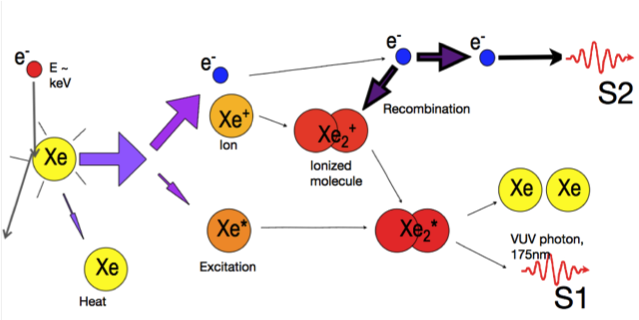
\includegraphics[width=120mm]{Figures/Tom_Shutt_ER_diagram.png}
\caption{Diagram of an electronic recoil in liquid xenon.}
\label{fig:TomS}
\end{figure}


Using equation \ref{eq:E_Q} and assuming that the heat loss is negligible for electronic recoils (ER) above 1 keV we can reconstruct energy by knowing the work function and the conversion from measured S1(light) and S2(charge) signals to the number of quanta ($\rm n_\gamma + n_e$) liberated by the interaction. We define gain-1 (g1) and gain-2 (g2) as the conversion from initial number of photons and electrons propagated from the interaction site to the observed signal by the PMT arrays as a photo electron (PE), given in equation \ref{eq:Gain1}. By using multiple mono energetic sources with know energies we can extract a best fit for the value of the gains (g1,g2) by making a Doke plot [ref]. The mono energetic lines used for the purposes of the calibration are listed in table \ref{table:Cal_lines}. For each calibration point we plot the mean S1/E vs. mean S2/E (Equation \ref{eq:Doke}) and fit a line, the x and y intercepts (Equation \ref{eq:LinFit}) yields the value of g1/W and g2/W respectively. The value of the work function W in liquid xenon has been found to be 0.0137 $\rm \pm$ 0.002  [ref]. The values of g1,g2 are degenerate and highly correlated such that the ratio of g1:g2 is always a constant, a reduction in g1 can be compensated by an increase in g2 and still yield the same number of initial quanta and visa versa. Breaking the degeneracy requires data over a wide range of S1 and S2 values near the intercept of the Doke plot. Due to the strong correlation in the fit parameters the data is fit by minimizing the likelihood and the errors in intercept and slope are determined using MCMC (Markov Chain Monte Carlo). 

\begin{equation}
\begin{split}
\rm  \left<n_\gamma\right> = \frac{\left<S1\right>}{g_1}\\
\rm \left<n_{e}\right> = \frac{\left<S2\right>}{g_2}
\label{eq:Gain1}
\end{split}
\end{equation}

\begin{equation}
\begin{split}
\rm  S1/E= \frac{n_\gamma}{(n_\gamma+n_e)}\times\frac{g1}{W} \\
\rm  S2/E= \frac{n_e}{(n_\gamma+n_e)}\times\frac{g2}{W}
\label{eq:Doke}
\end{split}
\end{equation}

\begin{equation}
\begin{split}
\rm  1= \left(\frac{S1}{E}\right)\left(\frac{W}{g1}\right) + \left(\frac{S2}{E}\right)\left(\frac{W}{g2}\right) \\[0.5ex]
\rm  \frac{S1}{E}=\frac{g1}{W} - \frac{S2}{E}\frac{g1}{g2} \\
\rm y=\frac{S1}{E}, x=\frac{S2}{E}, y= m\cdot x + b \\
\rm g1=b\cdot W \\
\rm g2=\frac{g1}{m}=\frac{b\cdot W}{m}
\label{eq:LinFit}
\end{split}
\end{equation}

\begin{table}[h!]
%\caption{Nonlinear Model Results}
\centering
\begin{tabular}{|c|c|c|}
\hline
Source & Energy [keV] &Decay Type  \\ [0.5ex] % inserts table %heading
\hline
Xe K shell  & 29.7, 34 	 		& X-ray							\\ \hline
 $\rm ^{83m}Kr$ 	& 41.55**		& Internal Conversion			\\ \hline
 $\rm ^{131}Xe$ 	& 163.9		& Internal Conversion			\\ \hline
$\rm ^{127}Xe$ 	& 203 or 375	& $\rm^{127}$I daughter $\rm \gamma$-emission	\\ \hline
				      & 33.8			& Kb shell X-ray 						\\ \hline
				      & 5.3			& L shell X-ray 					\\ \hline
$\rm ^{129m}Xe$	& 236.1		& Internal Conversion 			\\ \hline
$\rm ^{214}Bi	$	& 609 			& Inverse Beta Decay				 \\ \hline
 $\rm ^{137}Cs$	& 661.6		& Photo-absorption 					\\ [0.5ex] 
\hline
\end{tabular}
\caption{Mono energetic peaks used for g1 g2 calibration. ** Kr83 data was taken at 50 and 105 [V/cm] along with the standard field of 180 [V/cm].}
\label{table:Cal_lines}
\end{table}



\subsection{Anti-Correlation Space}
The first step in calibrating the energy scale is to plot the observables S1 vs. S2, by doing this the anti correlation between light and change at a given energy become apparent, figure \ref{fig:S1S2_space}. For the data presented here a fiducial cut was placed at a radius of less than 18 [cm] and drift distance between 6 and 46 [cm] which greatly reduces the background event rate. To extract g1 g2 we first determine the average values of S1 and S2 at each known energy. Initially loose diagonal cuts are placed by eye on the populations, figure \ref{fig:S1S2_space}. Next, using a un-binned maximum likelihood fit the mean and sigma are estimated and then refit using $\rm \pm 2\sigma$ of the initial distribution to remove tails from backgrounds. With the initial estimate for the mean S1 and S2 response to a given energy the gains g1,g2 are determined. The resulting value of g1 and g2 is found to be 0.096 $\pm$ 0.009 and 5.94 $\pm$ 1.68 respectively, the fit is shown in figure \ref{fig:Doke1}. The values of g1 and g2 represent a best fit tot he underling recombination theory where for each additional photon there is a corresponding reduction of one electron and visa versa. The method for extracting the uncertainties using MCMC will be discussed later in section \ref{sec:MCMC}.

\begin{figure}[h!]\centering
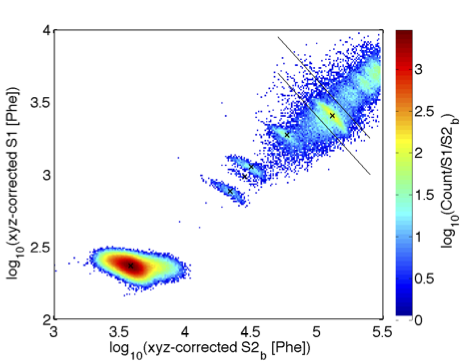
\includegraphics[width=80mm]{Figures/S1S2_density_Kr_Cs_fit.png}
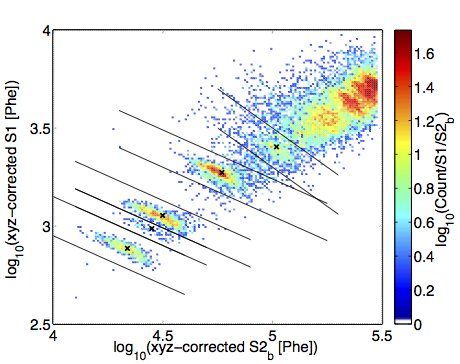
\includegraphics[width=80mm]{Figures/S1S2_density_XeA_fit.png}
\caption{LUX data in anti correlation space (S1 vs. S2), the black lines indicate the initial cuts by eye used to isolate populations of constant energy. In both figures diagonals represent lines of constant energy with a slope depending on the local recombination probability. The centroids found by an unbind maximum likelihood analysis are shows as a black X, for sources show in table \ref{table:Cal_lines}. }
\label{fig:S1S2_space}
\end{figure}

 \begin{figure}[h!]\centering
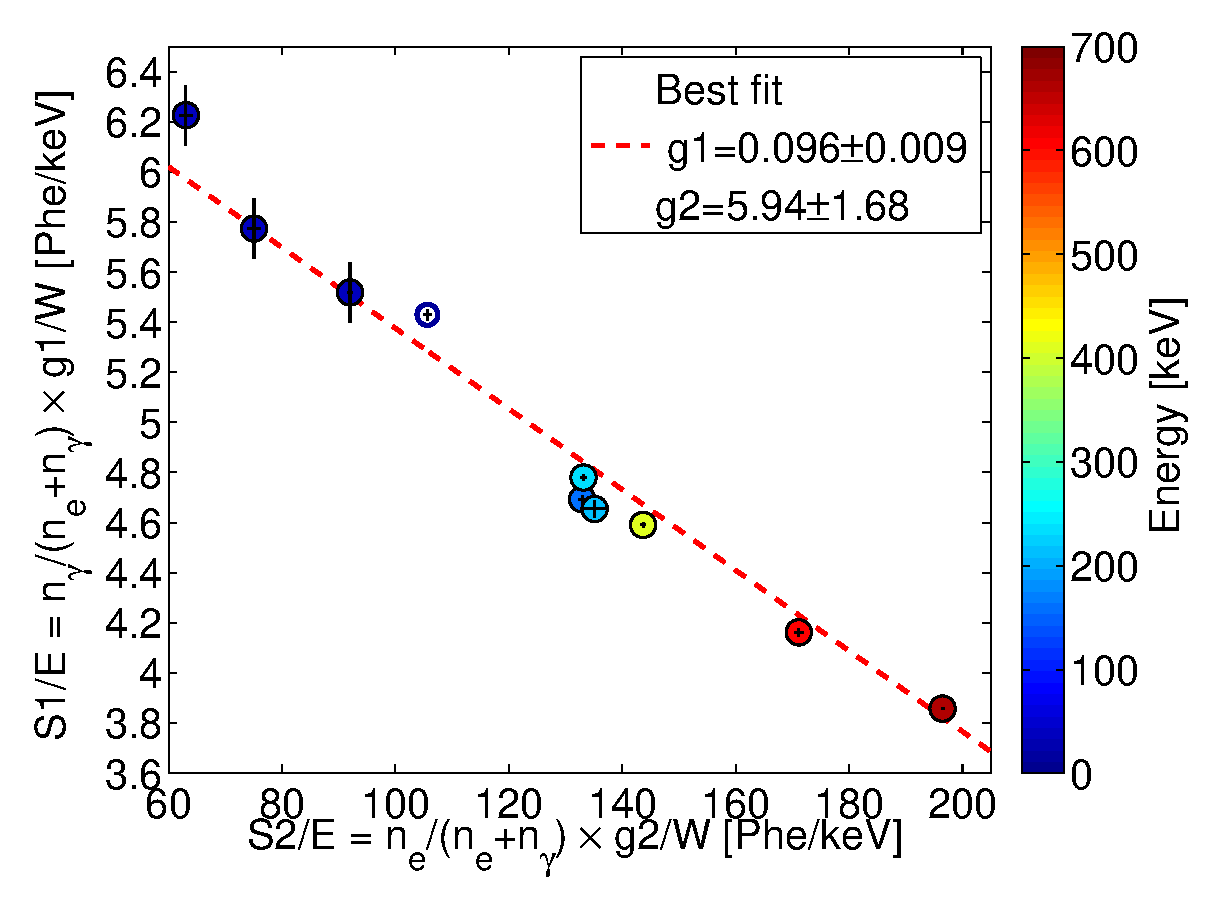
\includegraphics[width=120mm]{Figures/S1S2_Doke_1.eps}
\caption{Doke plot showing the best fit for the energy calibration parameters g1 and g2 using S1 and S2 means extracted from anti-correlation space. The first three blue points, from the left, are from $\rm^{83}Kr$ calibrations at 50, 105 and 180 V/cm respectively. The open circle was from the K-shell xenon X-ray and was not used for the fit as it's absolute energy and origin from the skin of the detector is uncertain.}
\label{fig:Doke1}
\end{figure}

\subsection{Refitting in Combined Energy Space}
From the first attempt to find g1,g2 we see, in figure \ref{fig:Doke1}, that there are discrepancies between the data and the fit, however this first result is only a crude estimate derived from anti correlation space. Once we have an initial estimate of gains g1,g2 a combined energy scale can be constructed with significantly improved resolution over the initial guess, due to the fact that recombination fluctuations are canceled. With the improved resolution the data are fit around the combined energy peaks using an unbinned maximum likelihood fit to a normal distribution, and then the data refitted around 1.5 $\sigma$ of the initial fit. The fits used to extract the means and sigmas  of the S1 and S2 signals at a given energy are show in figures \ref{fig:Doke_Fits_S1} and \ref{fig:Doke_Fits_S2}. We iterate this technique twice as the convergence is rapid, in this case the initial value of g1 and g2 derived from anti-correlation space are already a close approximation to the true value. The resulting value of g1 and g2 is found to be 0.097$\pm$0.008 and 5.75$\pm$1.4 respectively, the fit is shown in figure \ref{fig:Doke2}. After refitting there is a significant improvement over figure \ref{fig:Doke1}, especially the xenon activation lines in the center, which is due to better peak finding in combined energy space over anti-correlation space.


\begin{equation}
\begin{split}
\rm  g1 = 0.097\pm0.008 \\
\rm  g2= 5.75\pm1.4
\label{eq:g1g2Fit}
\end{split}
\end{equation}


 \begin{figure}[h!]\centering
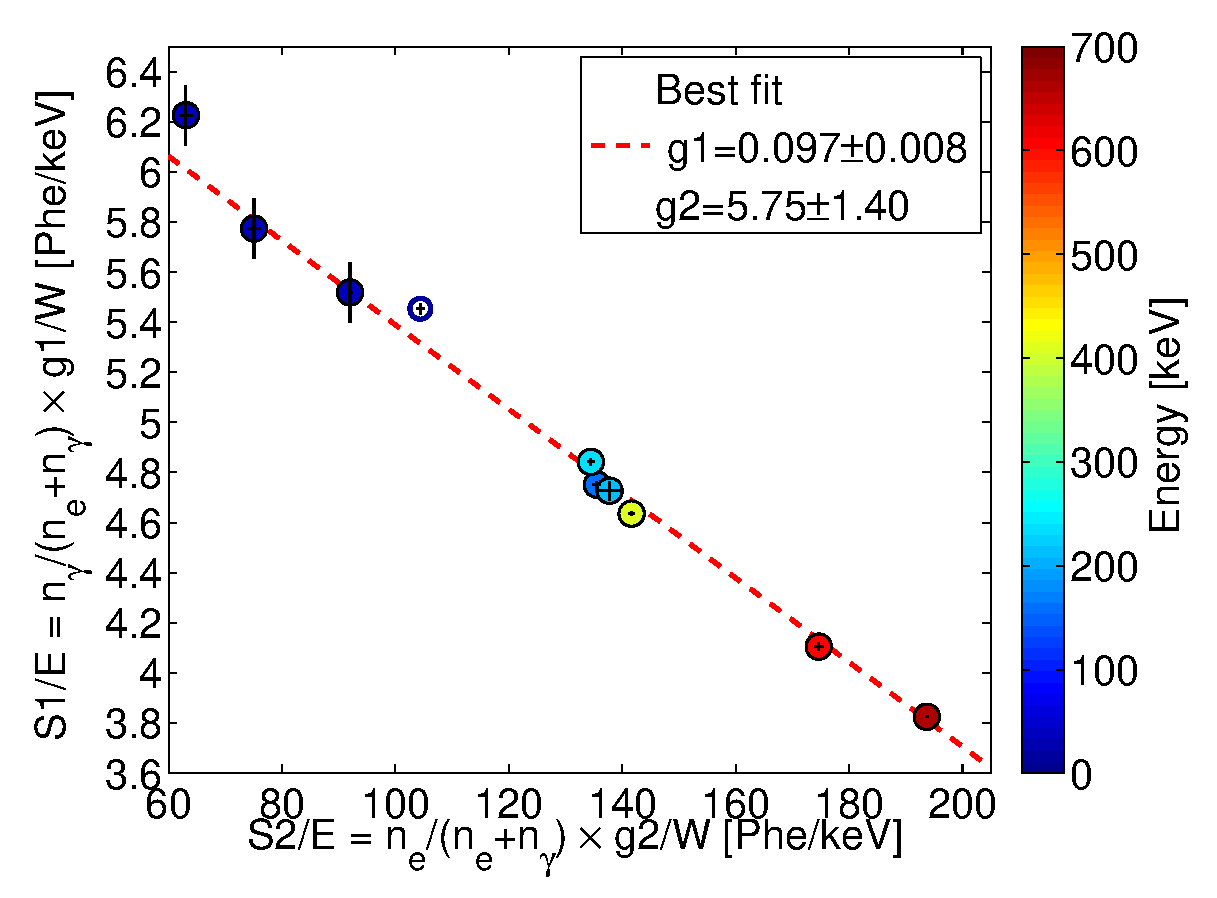
\includegraphics[width=120mm]{Figures/S1S2_Doke_3.eps}
\caption{Doke plot showing the best fit for the energy calibration parameters g1 and g2 using S1 and S2 extracted from a combined energy space. The first three blue points, from the left, are from $\rm^{83}Kr$ calibrations at 50, 105 and 180 V/cm respectively. The open circle was from the K-shell xenon X-ray and was not used for the fit as it's absolute energy and origin from the skin of the detector is uncertain.}
\label{fig:Doke2}
\end{figure}

 \begin{figure}[h!]\centering
 
\subcaptionbox{\label{fig:1a}}{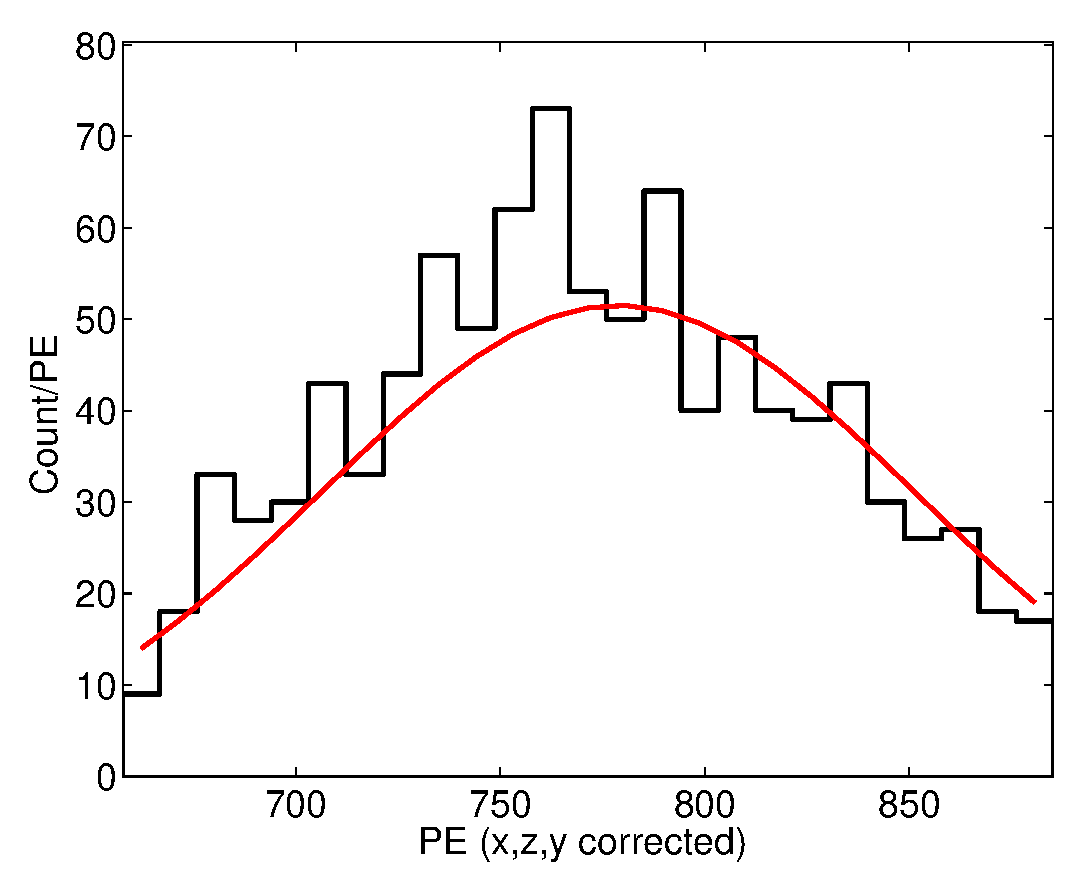
\includegraphics[width=50mm]{Figures/Doke_Fits/fit_S1_163.eps}}
\hfill
\subcaptionbox{\label{fig:1b}}{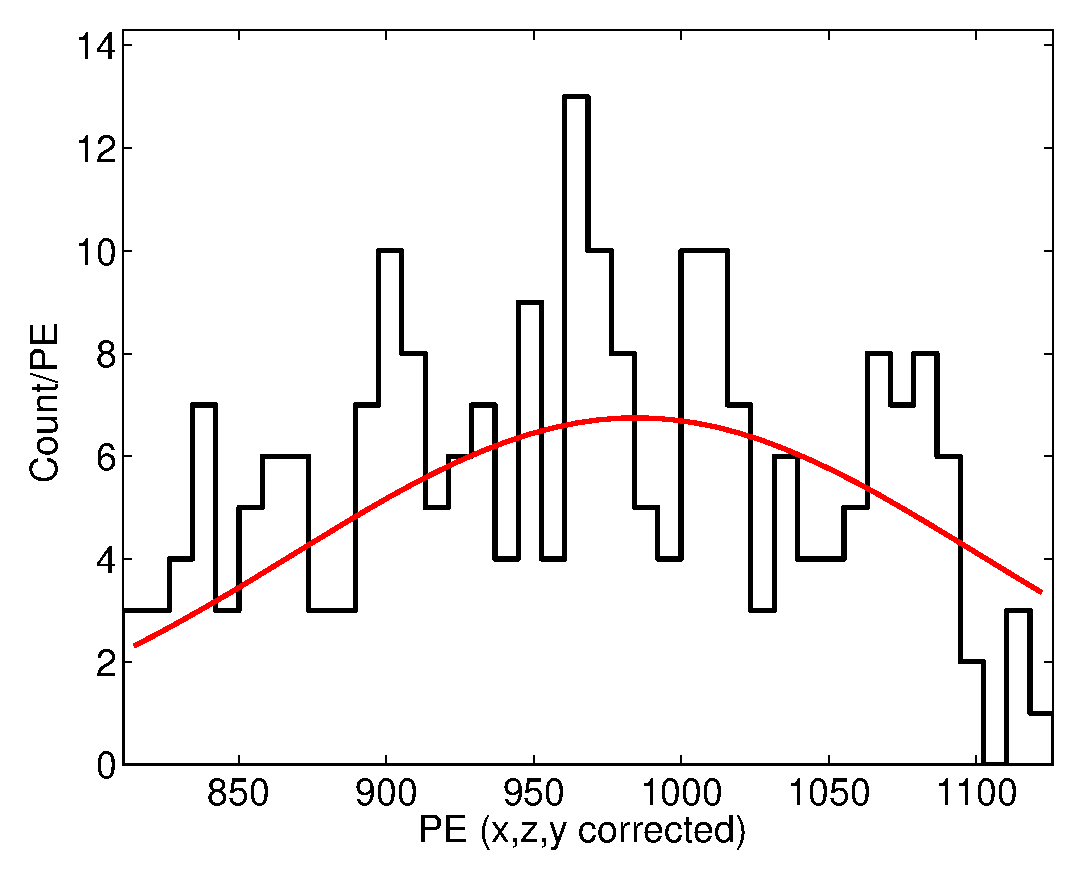
\includegraphics[width=50mm]{Figures/Doke_Fits/fit_S1_207.eps}}
\hfill
\subcaptionbox{\label{fig:1c}}{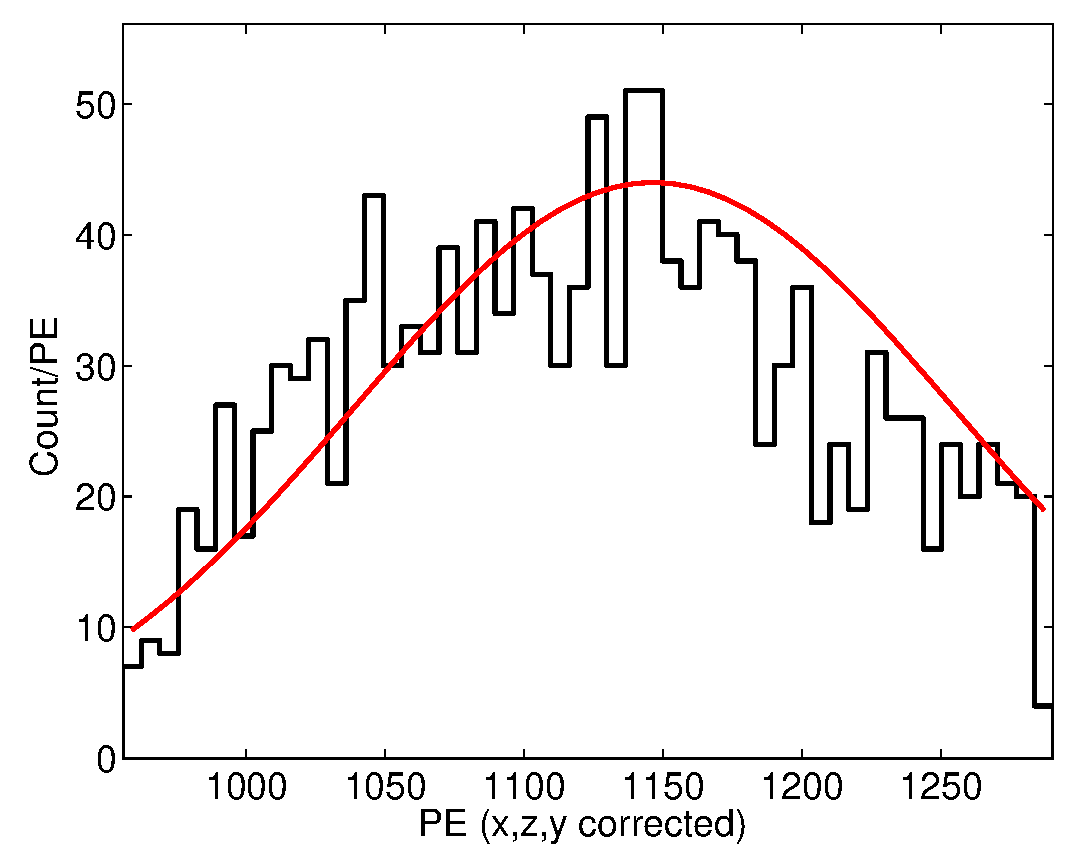
\includegraphics[width=50mm]{Figures/Doke_Fits/fit_S1_236.eps}}

\bigskip

\subcaptionbox{\label{fig:1d}}{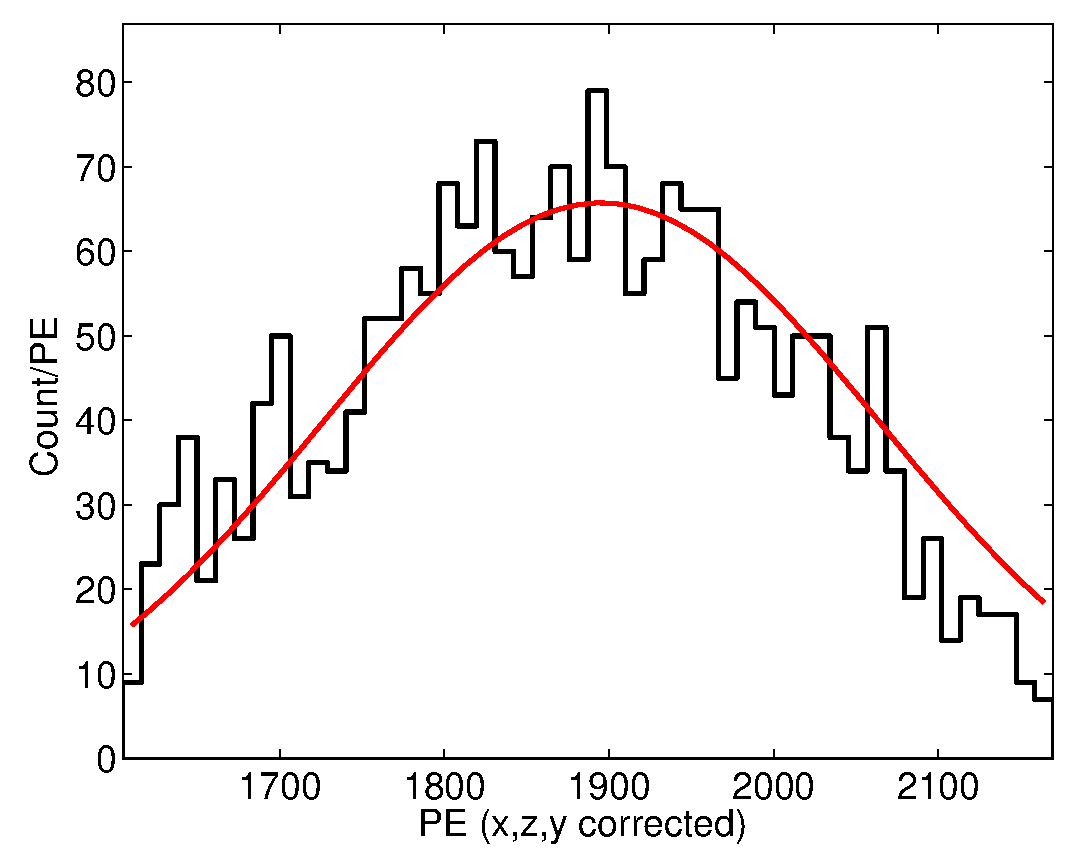
\includegraphics[width=50mm]{Figures/Doke_Fits/fit_S1_410.eps}}
\hfill
\subcaptionbox{\label{fig:1e}}{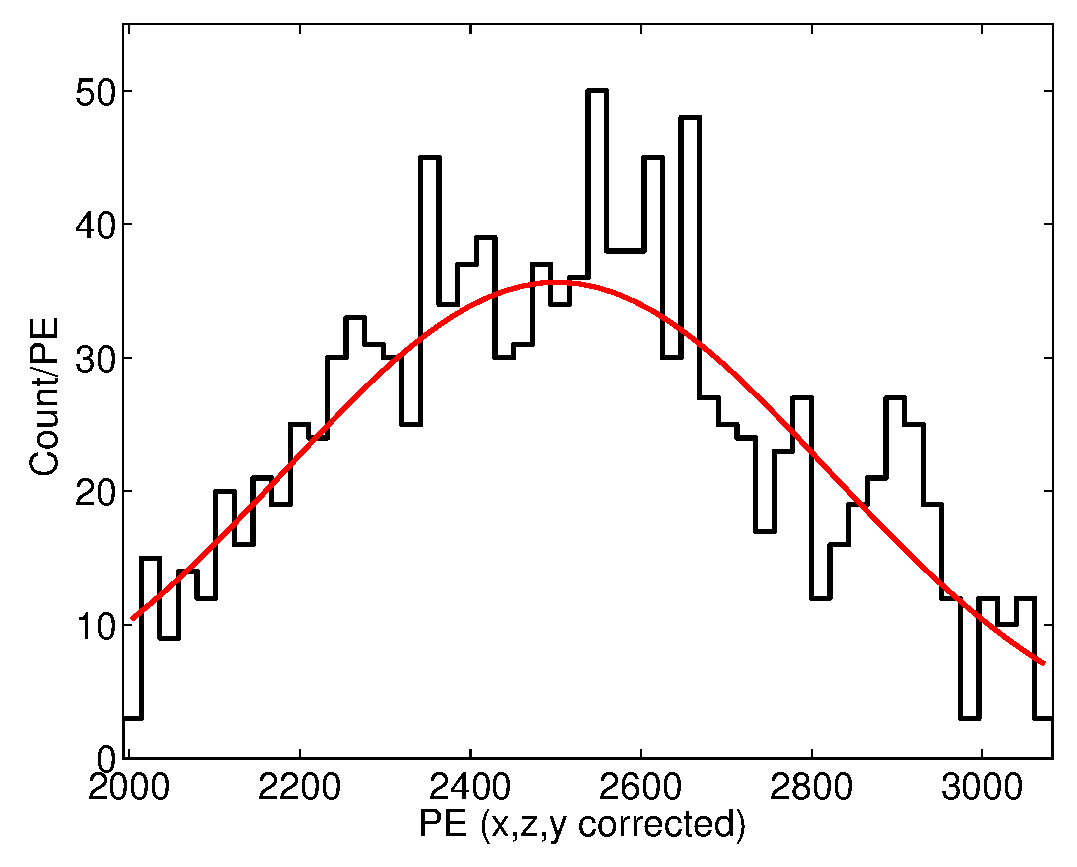
\includegraphics[width=50mm]{Figures/Doke_Fits/fit_S1_Bi214.eps}}
\hfill
\subcaptionbox{\label{fig:1f}}{\includegraphics[width=50mm]{Figures/Doke_Fits/fit_S1_Cs137.eps}}

\bigskip

\subcaptionbox{\label{fig:1g}}{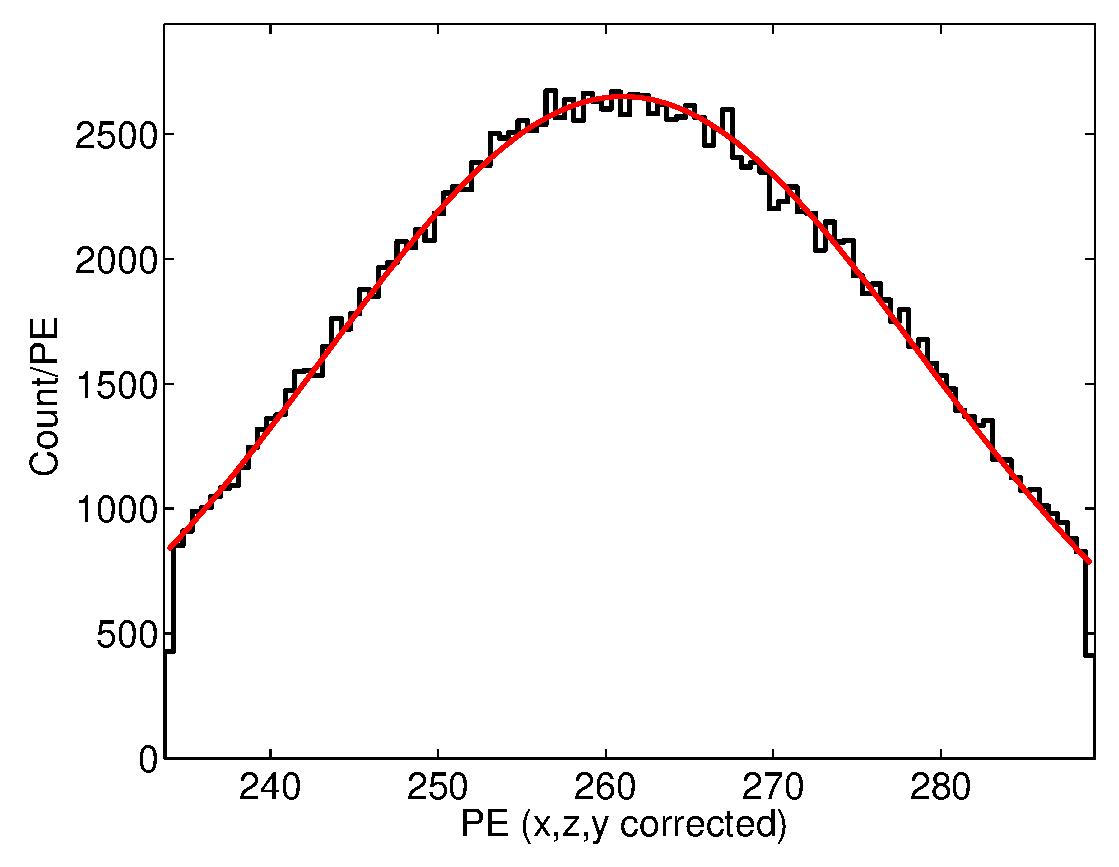
\includegraphics[width=50mm]{Figures/Doke_Fits/fit_S1_Kr_50.eps}}
\hfill
\subcaptionbox{\label{fig:1h}}{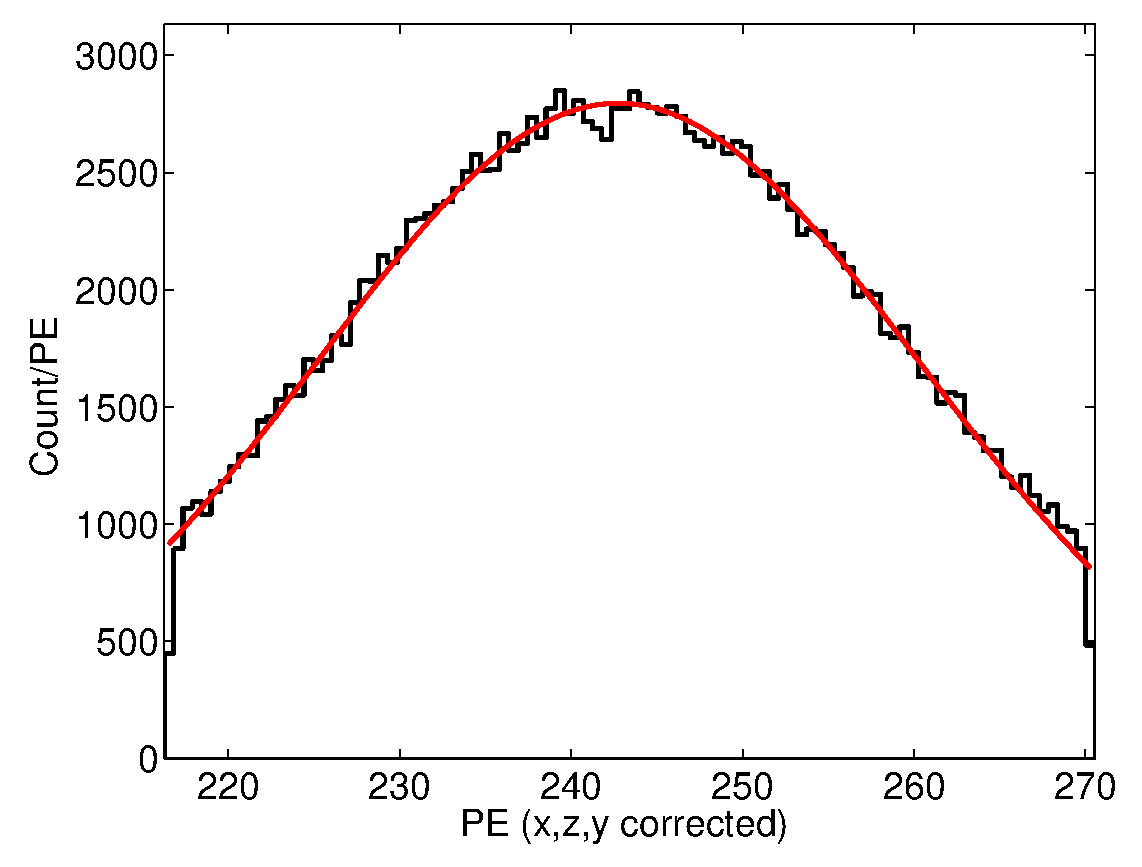
\includegraphics[width=50mm]{Figures/Doke_Fits/fit_S1_Kr_100.eps}}
\hfill
\subcaptionbox{\label{fig:1i}}{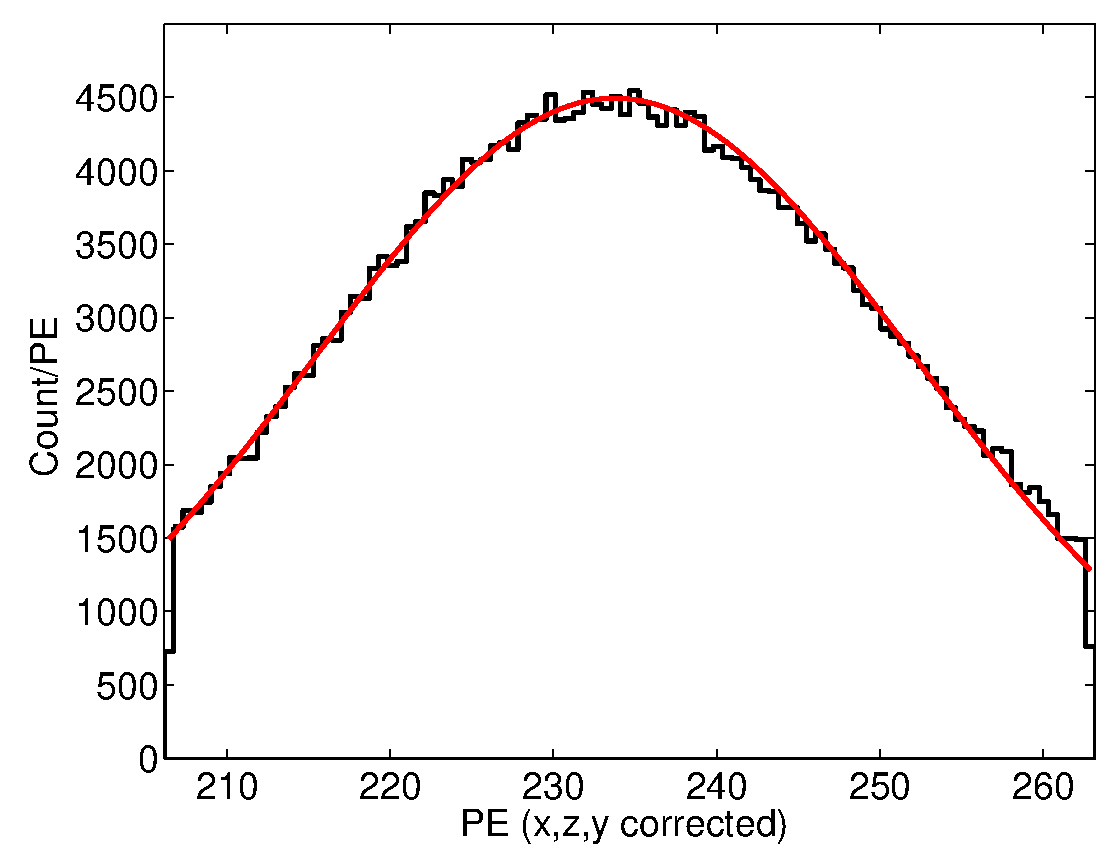
\includegraphics[width=50mm]{Figures/Doke_Fits/fit_S1_Kr.eps}}

\caption{S1 fits to sources at nominal field of 180 [V/cm] unless otherwise noted. Source and energy in keV from top left to bottom right: a) $\rm ^{131}Xe$: 163, b) $\rm ^{127}Xe$:  207, c) $\rm ^{127}Xe$ \&  $\rm ^{129m}Xe$: 236.8, d)  $\rm ^{127}Xe$: 410, e) $\rm ^{214}Bi$: 609, f) $\rm ^{137}Cs$: 661.6, g) $\rm ^{83m}Kr$: 41.5 - at 50 [V/cm], h) $\rm ^{83m}Kr$ 41.5 - at 105 [V/cm], i) $\rm ^{83m}Kr$ 41.5 .}
\label{fig:Doke_Fits_S1}
\end{figure}


 \begin{figure}[h!]\centering
 
\subcaptionbox{\label{fig:1a}}{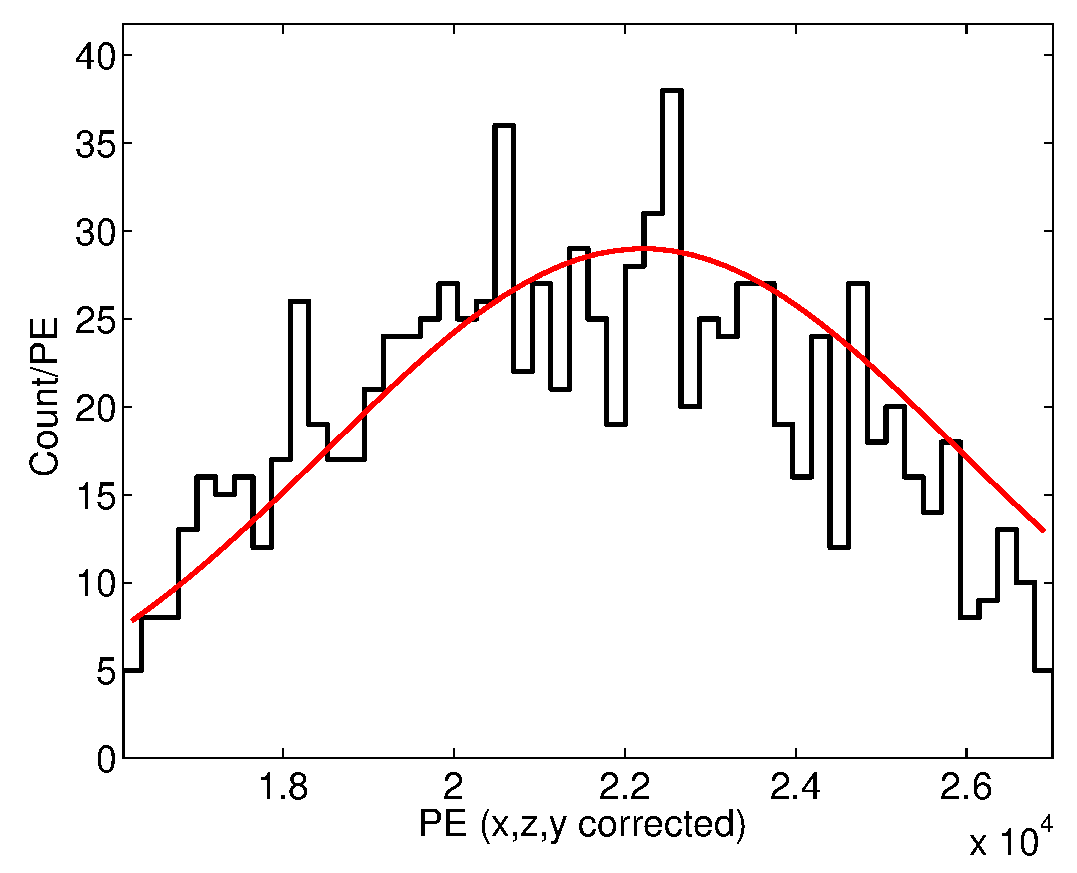
\includegraphics[width=50mm]{Figures/Doke_Fits/fit_S2_163.eps}}
\hfill
\subcaptionbox{\label{fig:1b}}{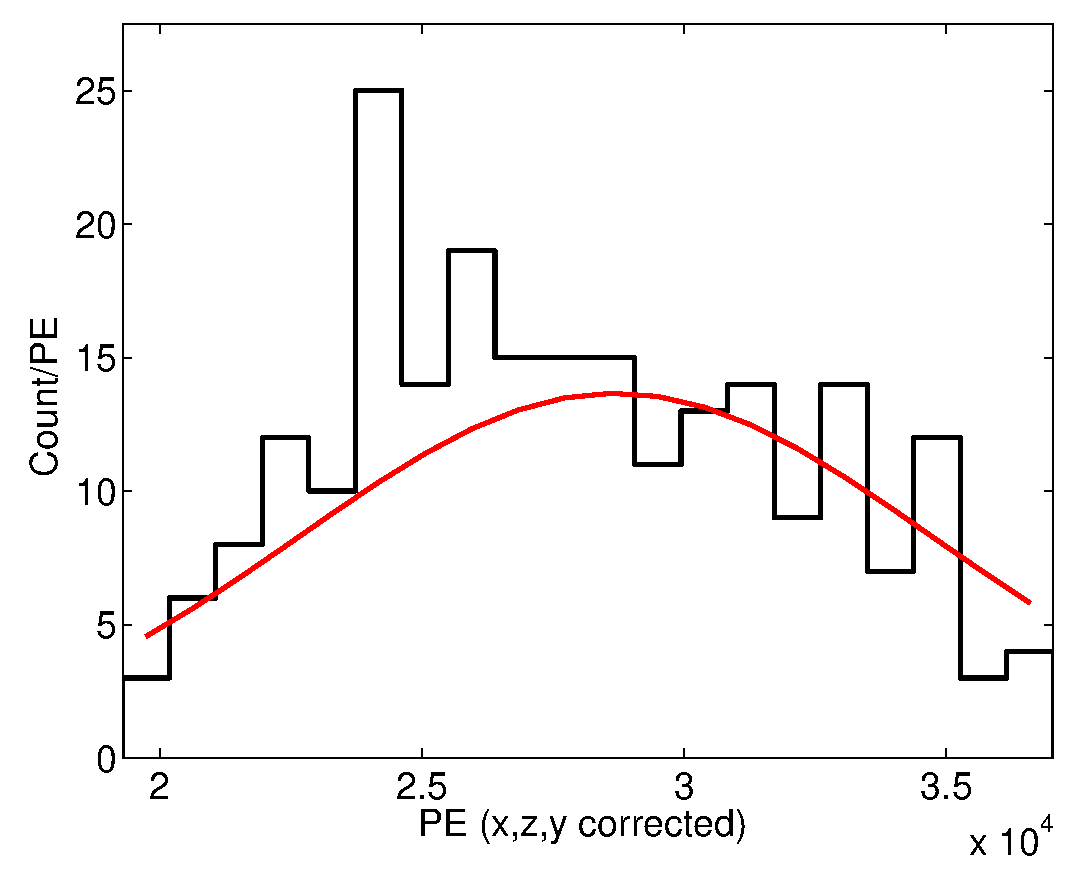
\includegraphics[width=50mm]{Figures/Doke_Fits/fit_S2_207.eps}}
\hfill
\subcaptionbox{\label{fig:1c}}{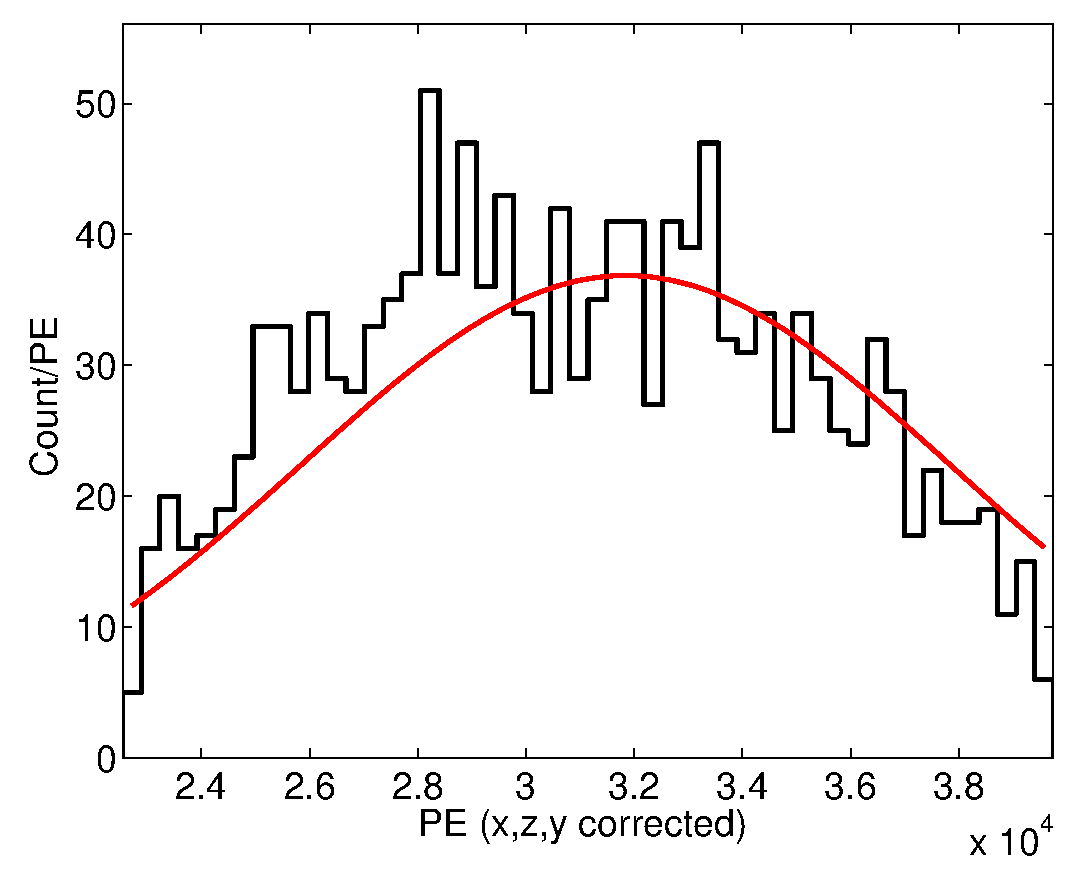
\includegraphics[width=50mm]{Figures/Doke_Fits/fit_S2_236.eps}}

\bigskip

\subcaptionbox{\label{fig:1d}}{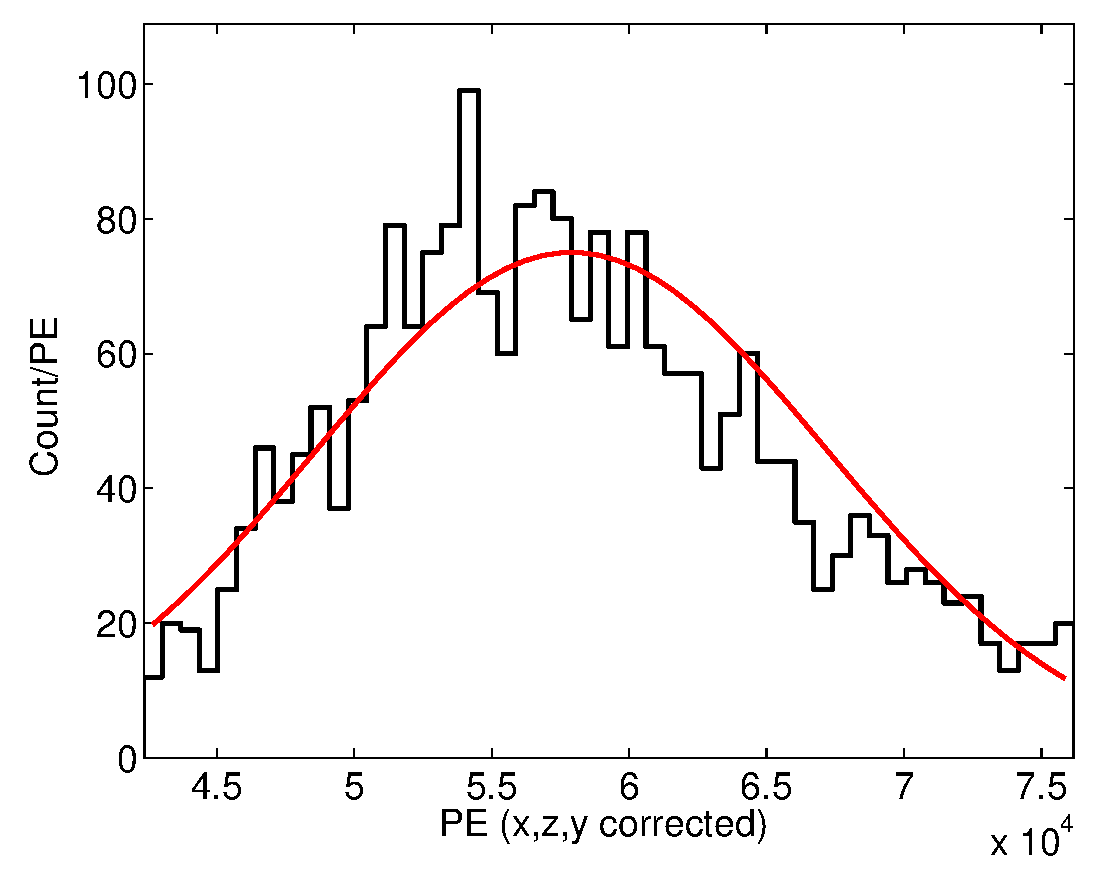
\includegraphics[width=50mm]{Figures/Doke_Fits/fit_S2_410.eps}}
\hfill
\subcaptionbox{\label{fig:1e}}{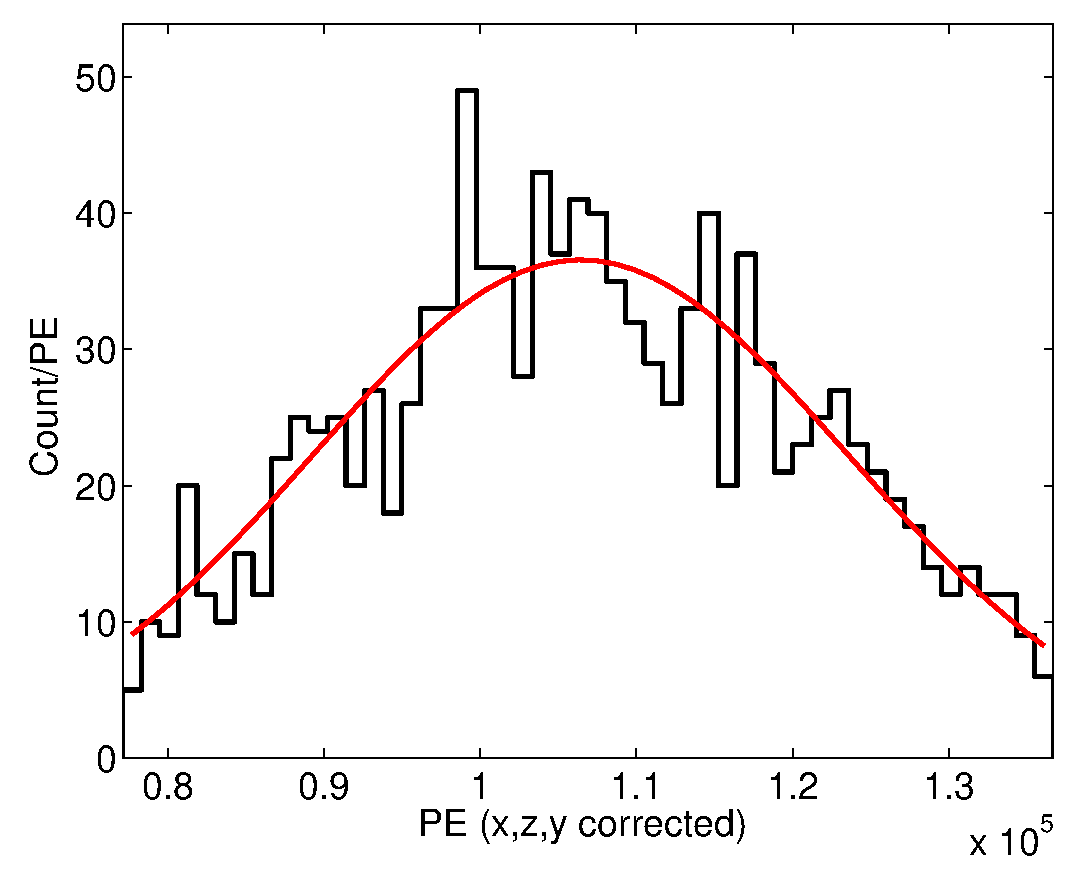
\includegraphics[width=50mm]{Figures/Doke_Fits/fit_S2_Bi214.eps}}
\hfill
\subcaptionbox{\label{fig:1f}}{\includegraphics[width=50mm]{Figures/Doke_Fits/fit_S2_Cs137.eps}}

\bigskip

\subcaptionbox{\label{fig:1g}}{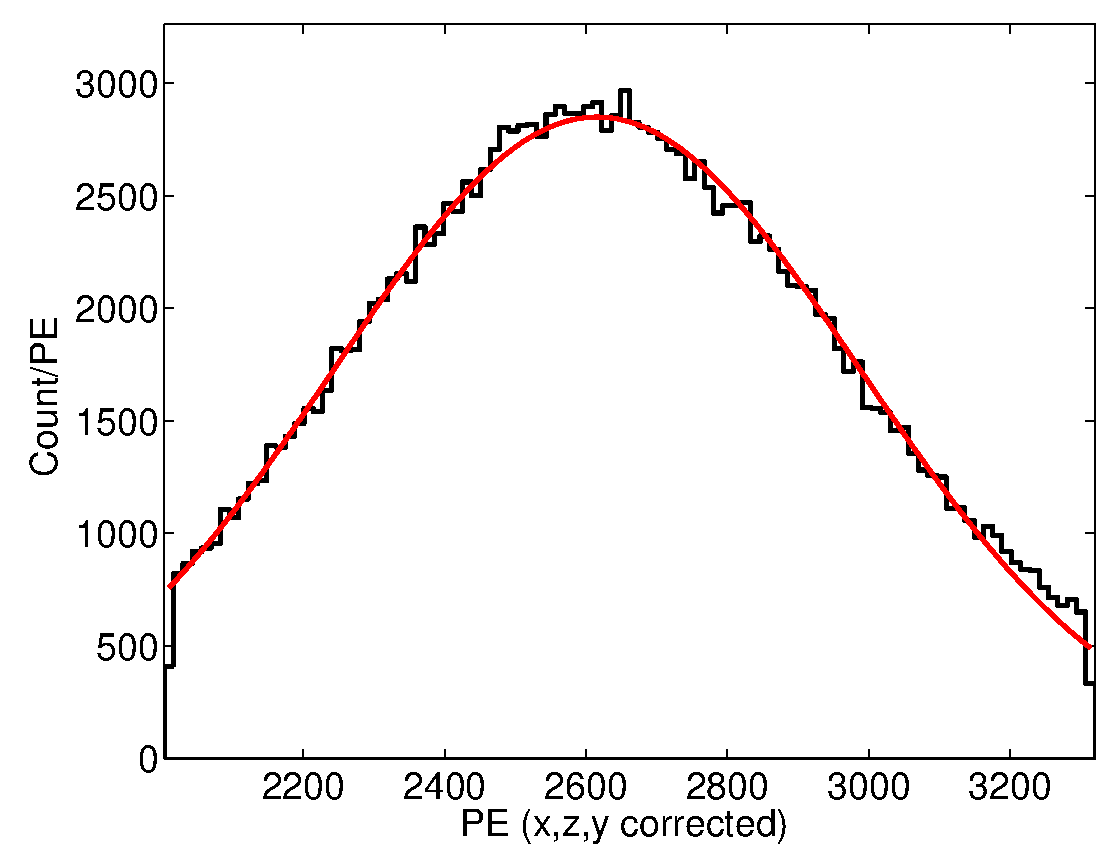
\includegraphics[width=50mm]{Figures/Doke_Fits/fit_S2_Kr_50.eps}}
\hfill
\subcaptionbox{\label{fig:1h}}{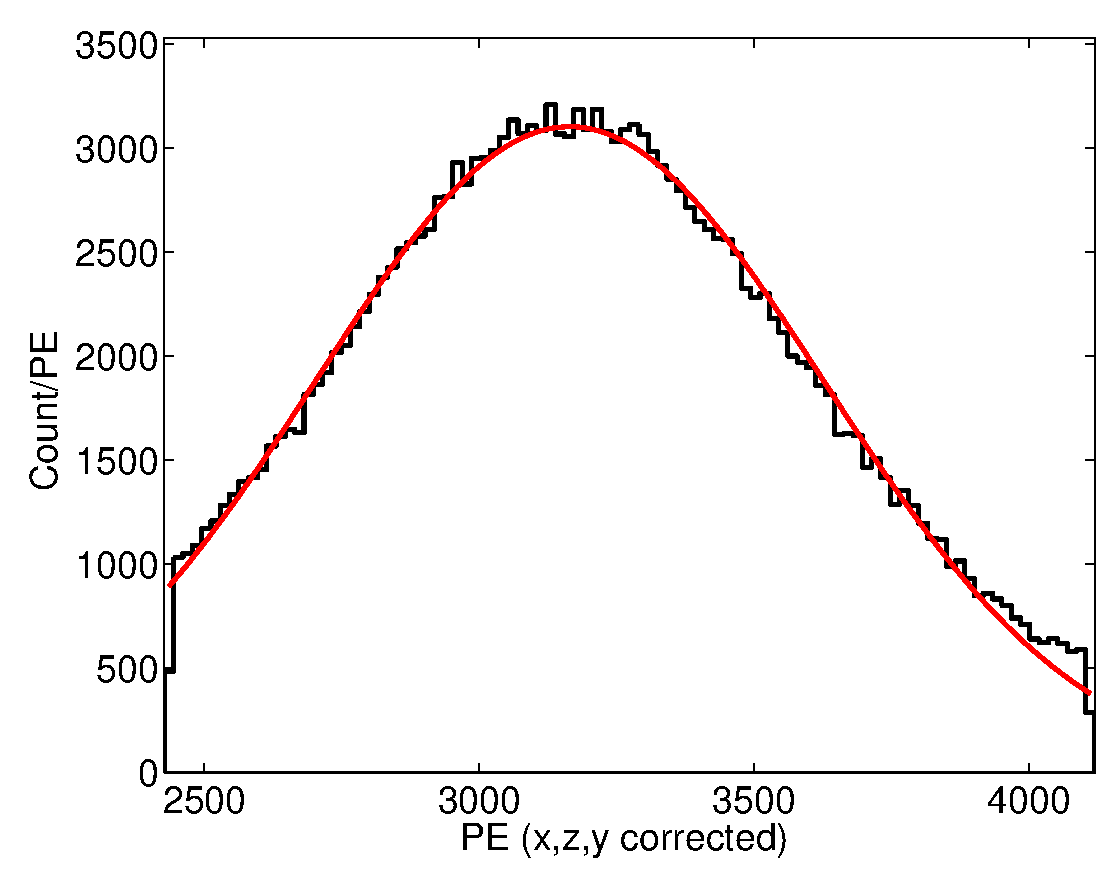
\includegraphics[width=50mm]{Figures/Doke_Fits/fit_S2_Kr_100.eps}}
\hfill
\subcaptionbox{\label{fig:1i}}{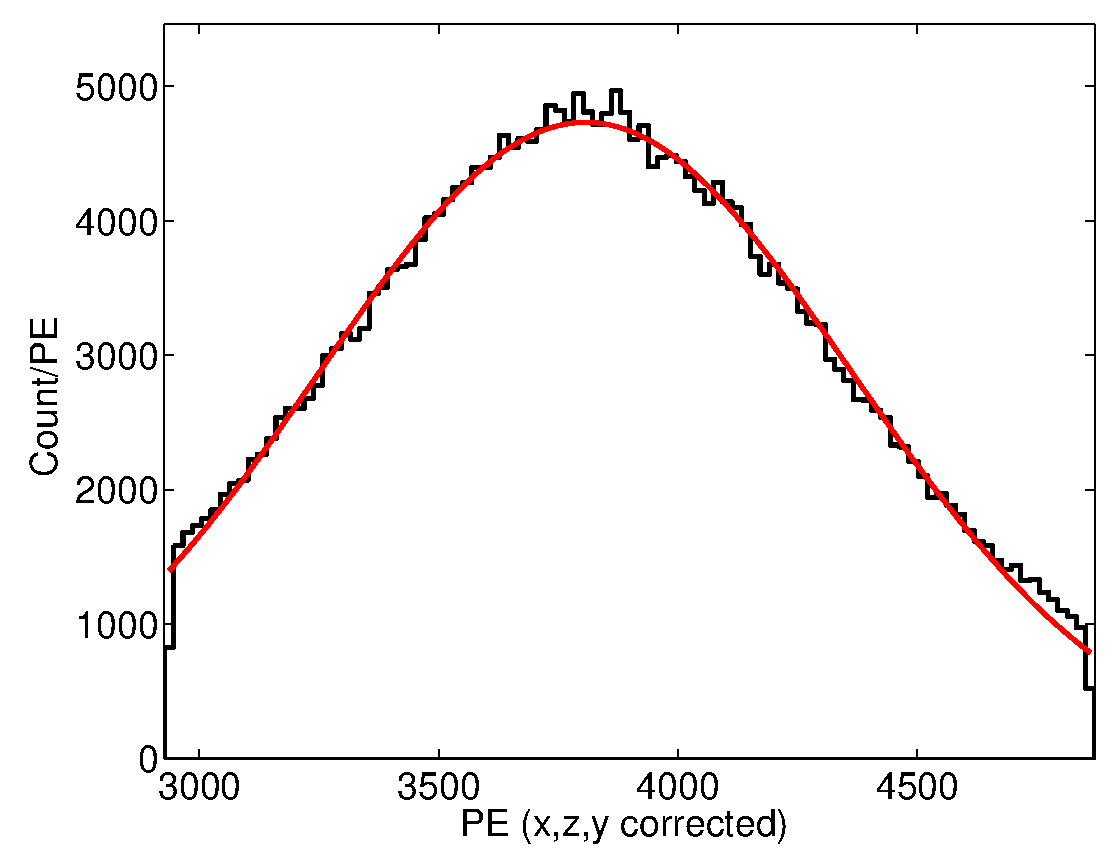
\includegraphics[width=50mm]{Figures/Doke_Fits/fit_S2_Kr.eps}}

\caption{S2 fits to sources at nominal field of 180 [V/cm] unless otherwise noted. Source and energy in keV from top left to bottom right: a) $\rm ^{131}Xe$: 163, b) $\rm ^{127}Xe$:  207, c) $\rm ^{127}Xe$ \&  $\rm ^{129m}Xe$: 236.8, d)  $\rm ^{127}Xe$: 410, e) $\rm ^{214}Bi$: 609, f) $\rm ^{137}Cs$: 661.6, g) $\rm ^{83m}Kr$: 41.5 - at 50 [V/cm], h) $\rm ^{83m}Kr$ 41.5 - at 105 [V/cm], i) $\rm ^{83m}Kr$ 41.5 .}
\label{fig:Doke_Fits_S2}
\end{figure}



Figure \ref{fig:Doke_E} is the final Doke plot for multiple peaks the theory describes the data well using the optimal fit for g1 and g2, for each increase in number of photons there is a corresponding decrease in the number of electrons and visa versa. The relatively large error on g2 is due to the distance of the data points from the x-intercept. As stated before the values of g1 and g2 can be locally degenerate as long as their ratio remains a constant. Thus for future studies it will be important to probe more of the parameter space in order to place a tighter constraint on gains g1 and g2.


 \begin{figure}[h!]\centering
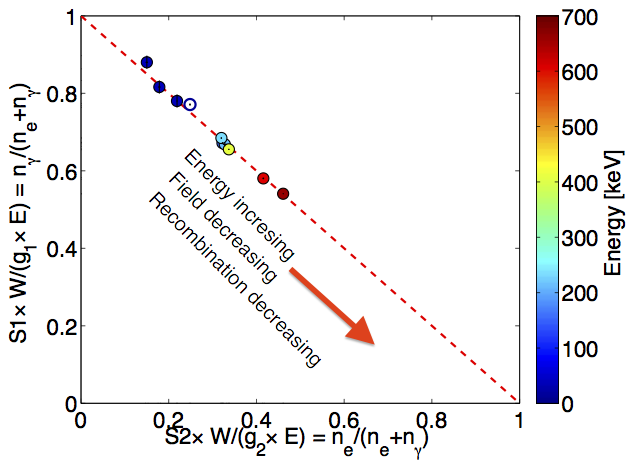
\includegraphics[width=100mm]{Figures/S1S2_Doke2_3_arrow.png}
\caption{Doke plot of the data.  Light yield vs. charge yield.}
\label{fig:Doke_E}
\end{figure}

\newpage

\subsection{Finding Errors with MCMC}
\label{sec:MCMC}
The error bars reported in this section on g1 and g2 are from the error in the slope and intercept of the linear fit in the Doke plot derived using MCMC. For calculating the error in slope and intercept  three random walkers were used at each data point and allowed to take 500 steps.The MCMC takes into account the covariance of the parameters, shown in figure \ref{fig:MCMC} as a two dimensional Gaussian. There is a strong negative correlation between the slope m and intercept b which is the result of the degeneracy between gains g1 and g2 used to reconstruct energy by combining the light and charge signal. Thus, the error on g1 and g2 is such that for the positive maxima deviation in g1 we reach the negative maxima of the error on g2, and visa versa. Using standard reduced $\chi^2$ for fitting and calculating errors in the slope and intercept would be underestimated the true error by a factor of five as it does not account for the degeneracy of the anti-correlated gains. 



\begin{figure}[h!]\centering
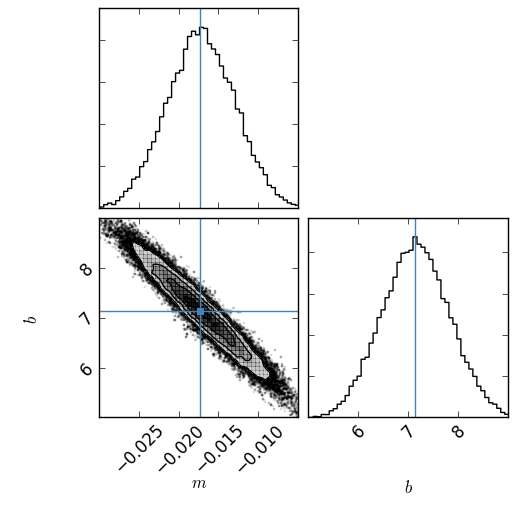
\includegraphics[width=100mm]{Figures/MCMC/triangle.png} % also line-time.png
\caption{MCMC for the linear fit to the Doke plot. There is a strong negative correlation between the slope m and intercept b which results from the degeneracy between gains g1 and g2. }
\label{fig:MCMC} 
\end{figure}

\newpage

\subsection{Combined Energy Space}

With the values of g1 and g2 known the combined energy of events can be reconstructed with a significant improvement over using only the light or charge channel. In combined energy space recombination fluctuations are removed by the anti correlation of light and charge production and any residual smearing is due to intrinsic detector resolution (discussed later in section :) . Figure \ref{fig:CE_hist} shows the energy histograms of the data used for the fits to gains g1 and g2 including the xenon activation lines and the $\rm^{137}Cs$ calibration, along with a zoom in of the xenon K shell Xray at 34 keV and a 81 keV gamma from $\rm ^{133}Xe$, not used for finding g1,g2. With the energy scale calibrated we can now reconstruct the energy of the events and convert the measured S1 and S2 signals to fundamental quanta using  the gains g1,g2 allowing us to untangle instrumental and recombination fluctuations and measure light and charge yields.


\begin{figure}[h!]\centering
 
\subcaptionbox{\label{fig:1a}}{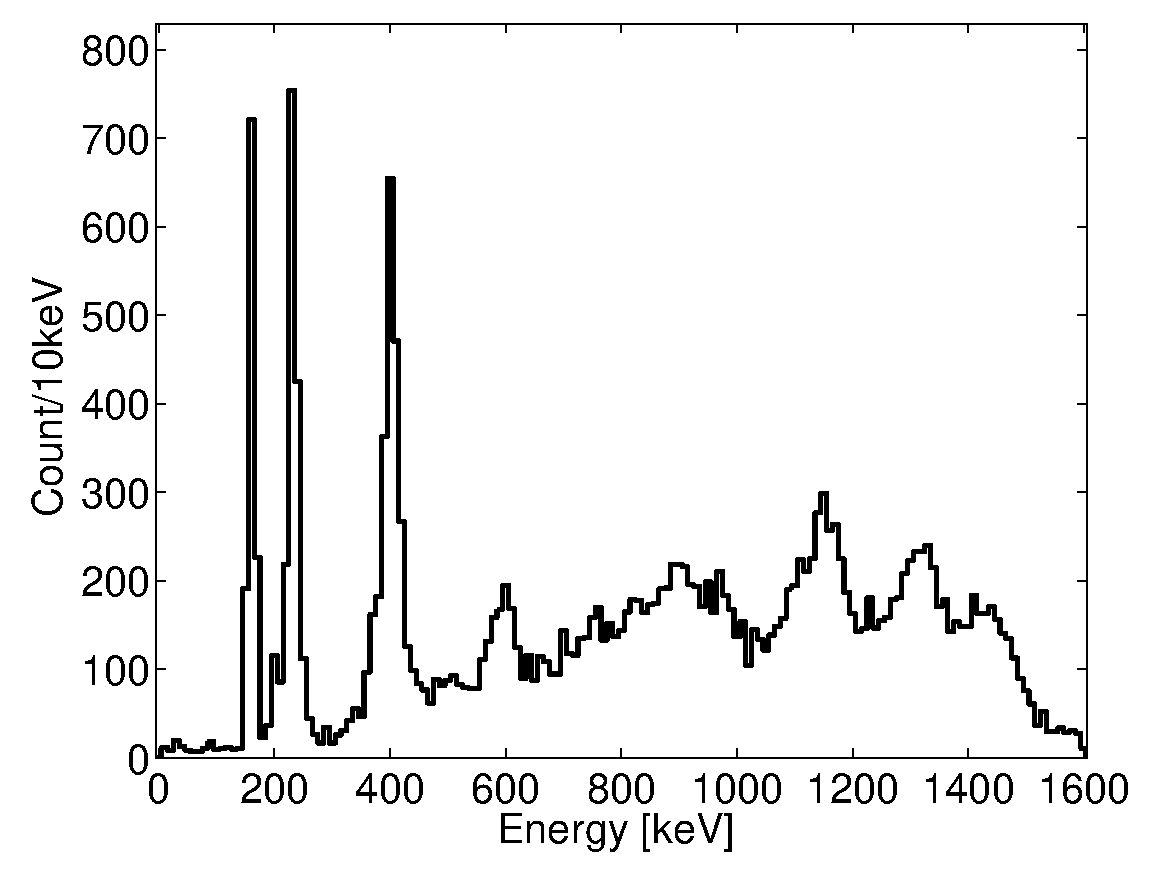
\includegraphics[width=70mm]{Figures/Combined_E/Xe_act_E.eps}}
\hfill
\subcaptionbox{\label{fig:1b}}{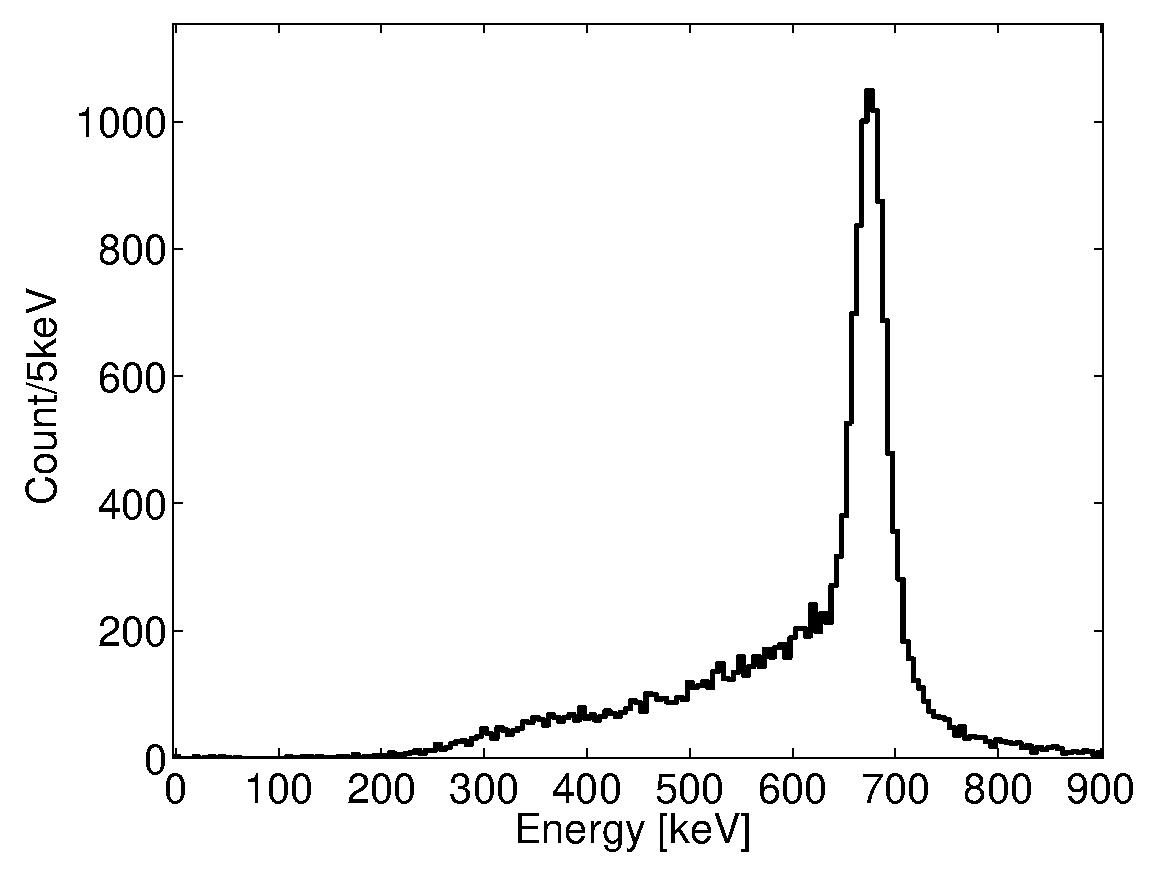
\includegraphics[width=70mm]{Figures/Combined_E/Cs_E.eps}}


\bigskip

\subcaptionbox{\label{fig:1c}}{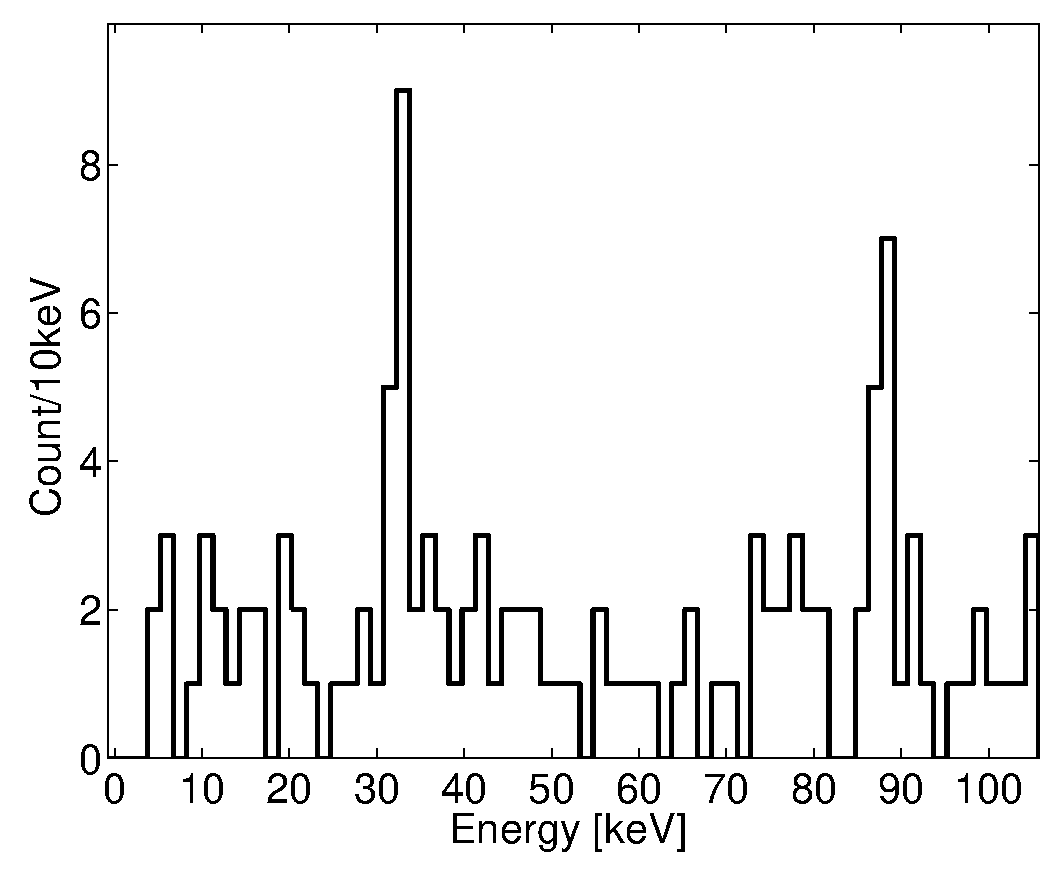
\includegraphics[width=70mm]{Figures/Combined_E/Xe_act_133_E.eps}}
\hfill
\subcaptionbox{\label{fig:1d}}{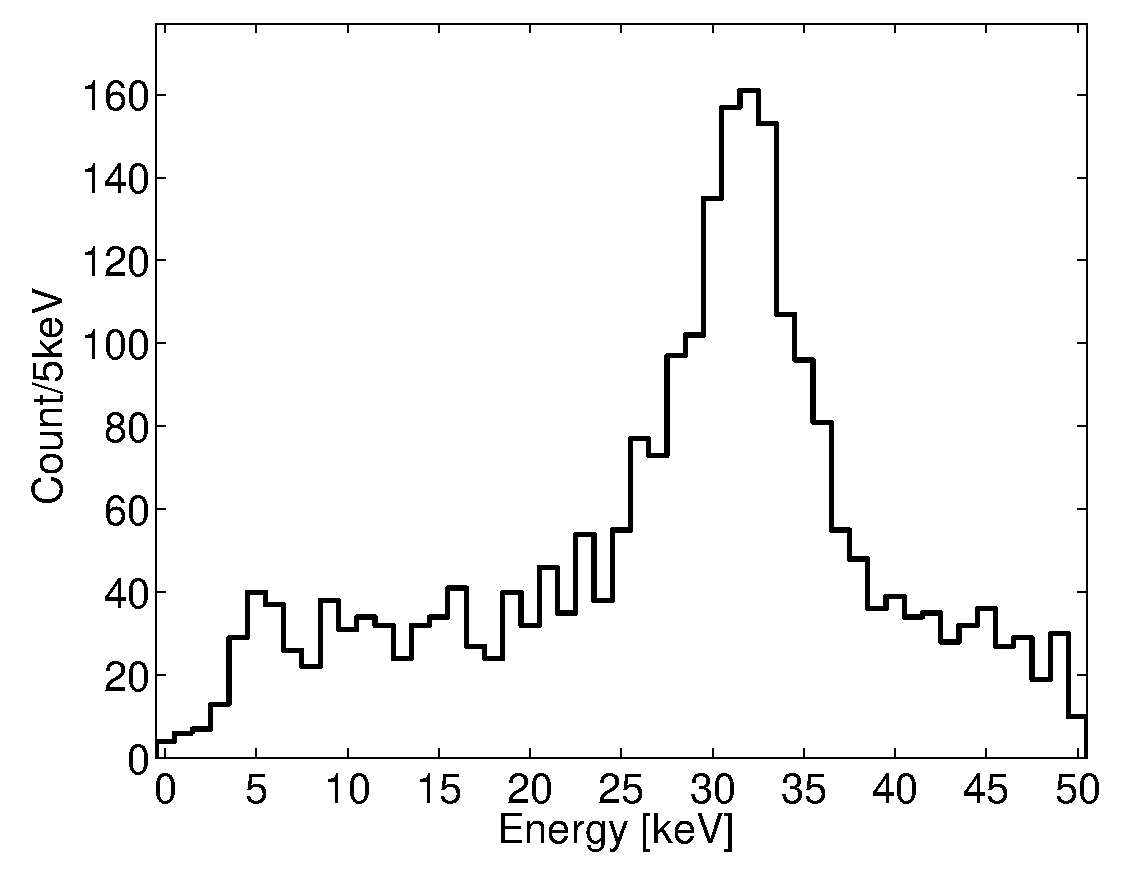
\includegraphics[width=70mm]{Figures/Combined_E/X-ray_Xe_E.eps}}


\caption{Combined energy scale. a) The xenon activation lines from early in the run. b) $\rm^{137}Cs$ calibration data. c) Xenon X-ray from the teflon skin (radium cut increased to the detector edge). d) Xenon X-ray and $\rm^{133}Xe$ at 81 keV, due to low stats was not used for fitting.}
\label{fig:CE_hist}
\end{figure}




\subsection{Light Collection and Electron extraction}

The value of g1 represents the mean efficiency for collecting photons at the center of the LUX detector, the response to S1 light is flat fielded and normalized to the detector center (section Kr calibrations). The measured value of g1= $\rm0.097\pm0.008$ implies a 9.7\% probability of a photon propagated from the center of the detector sticking a PMT and being converting into a photo electron (PE) signal. The value of g2 represents the average number of PE collected for each electron that escaped recombination at the initial interaction site then drifted by the electric field towards liquid-gas interface where it is extracted. Note, S2 signals are corrected for depth as impurities exponentially attenuate electrons drifting through the xenon (section Kr cal). Due to electo-lumanesance the S2 signal is such that a single extracted electron creates tens of photons which are collected by both PMT arrays. In our analysis we can cut on the single electron population (small S2 pulses without an associated S1) and measure the single electron size along with the extraction efficiency efficiency. The extraction efficiency is defined as the probability that an election will be extracted from the liquid into the gas in a region of 3.5 kV between the anode and the gate. For a given event the extraction of electrons is a binomial processes with a rate approaching unity for fields above 5 kV (reference). Figure \ref{fig:SingleE}, shows the single electron size as measured by the bottom PMT array (used for S2 pulses in the LUX detector to avoid saturation). The population is modeled by a skew Gaussian due to the Poisson nature of measuring only a handful of photo electrons (PE) per extracted electron. The mean of the distribution is found to be 9.7 PE/$\rm e^-$ with a width of $\rm \sigma SE$= 3.6 Phe/$\rm e^-$. Thus, the extraction efficiency is g2 over the single electron size 59.3\%, which given the extraction field is in good agreement measurements in other xenon detectors -[2 refs extraction].

\begin{figure}[h!]\centering
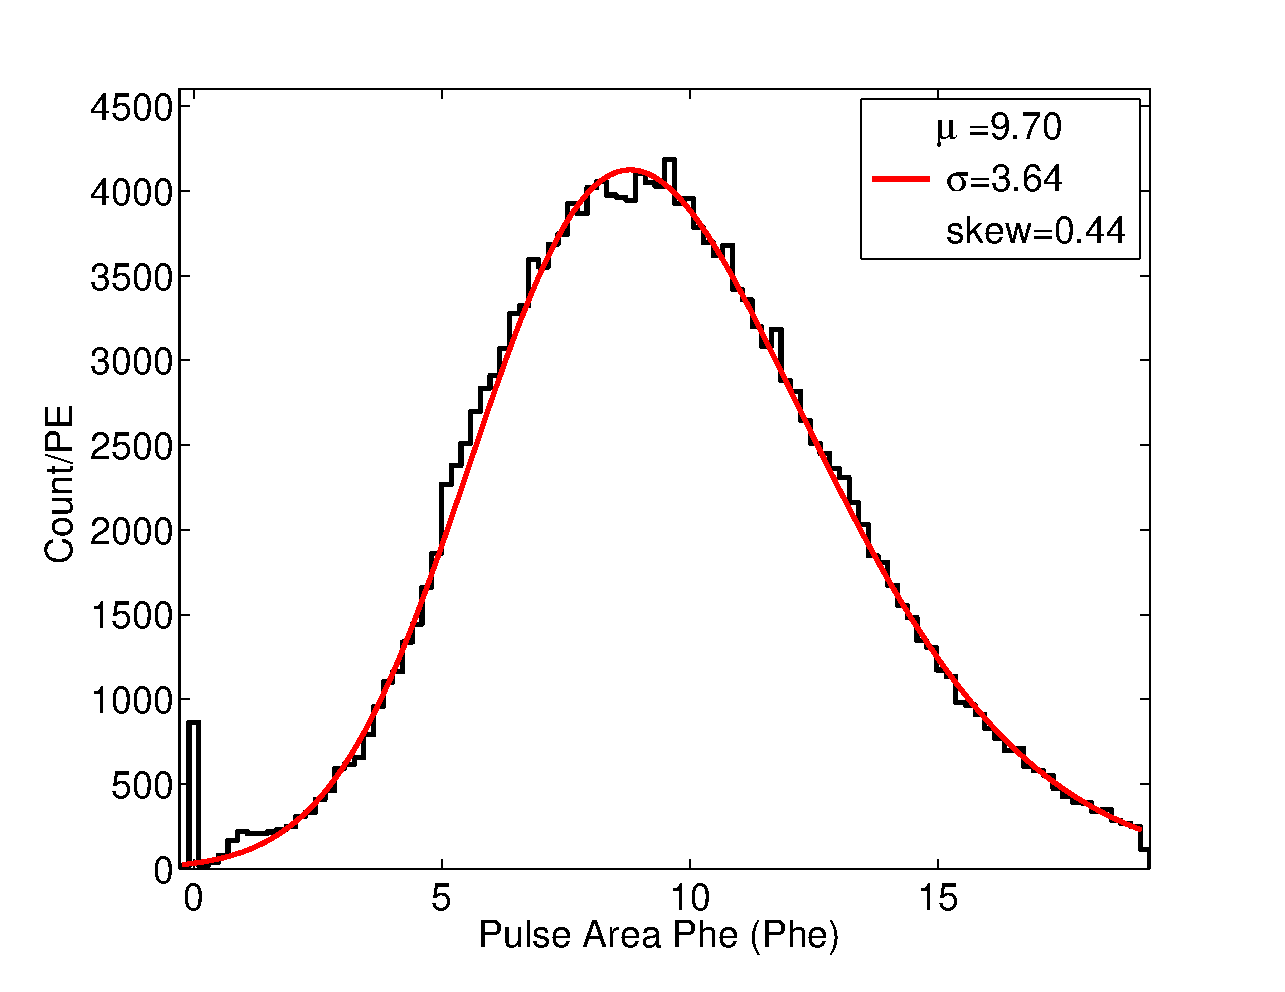
\includegraphics[width=100mm]{Figures/bottom_SE.eps}
\caption{Single electron distribution as seen by the bottom PMT array fitted with a skew Gaussian model to account for the underling Poisson statistics of observing between 9 and 10 photo electrons (PE) for each electron leaving the liquid and entering to the gas phase at a higher field causing electro-luminescence. The $\rm \mu$ of the fit represents the true mean of the skew Gaussian distribution. }
\label{fig:SingleE}
\end{figure}

\section{Modeling Intrinsic Detector Resolution}

Intrinsic statistical fluctuations in light and charge (S1, S2) collection in the LUX detector lead to a spread in collected quanta. To measure effects from recombination fluctuations and the Fano factor we must first decouple the detector component of resolution. We use the model described in [Dahl's thesis] in which the measured scintillation and ionization signals S1, S2 (measured in Phe) are related to the number of photons and electrons by gains g1 and g2, \ref{eq:Gain}. Specifically, the average number of photons and electrons produced for a given energy deposit are proportional to the average S1,S2 signals at a given drift field. The gain g1 represents photon detection efficiency, the probability of a photon from an energy deposit striking a PMT convolved with the quantum efficiency of the PMTs. Gain g2 represents the average S2 signal of a single electron normalized by the average single electron size. Where S2 uses only the bottom PMT array and is corrected for lifetime.


\begin{equation}
\begin{split}
\rm  \left<n_\gamma\right> = \frac{\left<S1\right>}{g_1}\\
\rm \left<n_{e}\right> = \frac{\left<S2\right>}{g_2}
\label{eq:Gain}
\end{split}
\end{equation}

The statistical fluctuations for the measured number of quanta in equation \ref{eq:Gain} are from the statistical processes that comprise the measured S1 and S2 signal.

\begin{equation}
\begin{split}
\rm  \sigma_{n_{\gamma_{stat}}}^2 = \frac{\sigma_{S1_{stat}}^2}{g_1^2}\\
\rm \sigma_{n_{e_{stat}}}^2 = \frac{\sigma_{S2_{stat}}^2}{g_2^2}
\label{eq:Sig}
\end{split}
\end{equation}

The variance in the number of photons in equation \ref{eq:Sig} can be broken into two parts. First, a binomial variance due to counting a fraction, g1, of the initial photons produced. $\rm Var_{n_\gamma} = \frac{(1-g1)\times g1\times n_\gamma}{g_1^2}$. Second, the variance in the response of the PMTs to a single photon. $\rm Var_{n_\gamma} = \frac{g_1\times n_\gamma \times \sigma_{PE}^2}{g_1^2}$. Combining the two leads to the the result in equation \ref{eq:Sig_S1}.

\begin{equation}
\rm  \sigma_{n_{\gamma_{stat}}}^2 = \frac{1-g_1+\sigma_{PE}^2}{g_1} n_\gamma\\
\label{eq:Sig_S1}
\end{equation}


The variance in the number of electrons in equation \ref{eq:Sig} is comprised of the following statistical uncertainties. First, a binomial variance due to the extraction efficiency of electrons from the liquid-gas interface. $\rm Var_{n_e} = \frac{(1-ext)\times Ext\times n_e \times(single_E)}{g_2^2}$, Ext is the electron extraction probability and $\rm single_E$ is the single electron size in PE. Second, the variance in the response of the PMTs to a single electron. $\rm Var_{n_e} = \frac{Ext\times n_e \times \sigma_{SE}^2}{g_2^2}$. Finally, the additional variance from electron attenuation is modeled as a Poisson probability of electron capture in each Z slice of the detector. The variance from each Z slice depends of the average number of electrons that will be attenuated. The probability of attenuation at each slice in drift time T is $\rm P(T)= 1-e^{-T/\tau}$, where $\rm \tau$ for the data sets to be considered is 1000 $\rm \mu s$. The drift region considered in the fiducial volume is from 38 to 304.5 $\rm \mu s$. The average variance from events in the fiducial can be given by equation \ref{eq:Sig_Att}.

\begin{equation}
\rm  \sigma_{n_{e_{att}}}^2 = n_e \frac{\mathlarger{\int}\limits_{\mathsmaller{T_{min}}}^{\mathsmaller{T_{max}}} (1-e^{-T/\tau})\mathrm{d}T}{\mathlarger{\int}\limits_{\mathsmaller{T_{min}}}^{\mathsmaller{T_{max}}}\mathrm{d}T} = 0.155 \times n_e
\label{eq:Sig_Att}
\end{equation}

Combining the variances leads to the the result for the statistical variance in the observed number of electrons equation \ref{eq:Sig_S2}.

\begin{equation}
\rm  \sigma_{n_{e_{stat}}}^2 = \frac{Ext \times \sigma_{SE}^2+(1-Ext)\times g2}{g_2^2} n_e +  \sigma_{n_{e_{att}}}^2\\
\label{eq:Sig_S2}
\end{equation}


For this analysis we use the following detector gains, given measured by comparing tritium data to the vetted region of LUXSIM (S1 between 7-50 Phe)   \ref{eq:g1g2}. 
\begin{multline} \\
\rm g_1 = 0.097 \pm 0.008 \,[Phe/n_\gamma]\\
\rm g_2=SE_{b} \times Ext = 5.75 \pm 1.4 \,[Phe/n_e]\\
\rm SE_{b} = 9.70 \pm 0.05  \,[Phe/n_e] \\\ 
\rm \sigma SE_b = 3.64\, [Phe/n_e]\\
\rm Ext = 0.593\pm 0.144 \\
\rm \sigma_{PE} = 0.51\, [Phe/n_\gamma]\\\
\label{eq:g1g2}
\end{multline}

Combining equations \ref{eq:Sig_S1}-\ref{eq:g1g2} we find the intrinsic detector resolution for the average S1 and S2 signals in the LUX detector, equation \ref{eq:SigStat}. Note, the intrinsic resolution in S2 is subdominant to that of S1, since  on average one electron multiplies to about ten photons detected by the bottom PMT array [ref]. Also listed in \ref{eq:SigInst}, are the instrumental fluctuations with a linear dependance on quanta measured with a global fit to mono energetic sources [next section]. The total variance in the light and charge channels is the linear combination of the statistical and instrumental variance.  

\begin{equation}
\begin{split}
\rm  \sigma_{n_{\gamma_{stat}}} = 3.46 \sqrt{n_\gamma}\\
\rm \sigma_{n_{e_{stat}}} = 0.68 \sqrt{n_e}
\label{eq:SigStat}
\end{split}
\end{equation}

\begin{equation}
\begin{split}
\rm  \sigma_{n_{\gamma_{inst}}} = \frac{6.4\pm 1.7}{100} \times n_\gamma\\
\rm  \sigma_{n_{e_{inst}}} = \frac{6.6\pm 0.9}{100} \times n_e
\label{eq:SigInst}
\end{split}
\end{equation}



\section{Measuring Recombination Fluctuations}

\subsection{Measuring Recombination Fluctuations with Mono-Energetic Sources}

To model recombination we start with a basic assumption that for a given energy deposit in liquid xenon the number of quanta produced is equal to the number of exitons and the number of ions. The number of ions cerated contains a spread given by a Fano factor F. The value of F for liquid xenon is small, has a theoretical value of 0.05 \cite{FanoTheoretical}.

\begin{equation}
\begin{split}
\rm  \frac{E}{W} = n_q = n_i + n_{ex}\\
\rm \frac{E}{W} = n_\gamma + n_e
\label{eq:Energy}
\end{split}
\end{equation}

Where E is energy in [keV], W is the work function in [keV/quanta], $\rm n_{q}$ is the number of quanta, $\rm n_{i}$ is the number of ions and $\rm n_{ex}$ is the number of exitons. The theoretical value of the number of exitons produced to ions is $\rm \frac{n_{ex}}{n_{i}}= \alpha = 0.06$ and is not expected to change vs. energy [ref]. For the subsequent equations in this section we will simplify equations \ref{eq:Energy} to that in \ref{eq:Energy_2}.

\begin{equation}
\begin{split}
\rm \alpha = 0.06\\
\rm  n_i = \frac{E}{W} \frac{1}{(1+\alpha)} =  \frac{n_\gamma + n_e}{(1+\alpha)}  \\ %  \frac{n_q}{(1+\alpha)}
\rm \sigma_{n_i}^2  = F \times n_i
\label{eq:Energy_2}
\end{split}
\end{equation}

Equation \ref{eq:Energy_2} gives us a simple model for the number of ions and exitons produced for a given interaction, the only spread in quanta thus far is due to a Fano factor governing the spread in initial quanta produced. We now convert ions and exitons to scintillation and ionization signals that are measured in the LUX detector, S1  and S2 respectively. Photons resulting from an energy deposit arise from the exitons that de-excite and from ions which recombine with freed electrons. The number of electrons corresponding to the energy deposit will be equal to the number of ions that did not recombine with a freed electron. 

\begin{equation}
\begin{split}
\rm  n_\gamma = n_{ex} + n_i\times r = n_i\times (r+\alpha) \\
\rm  n_e = n_i\times (1-r)\\
\rm r= \frac{\frac{n_\gamma}{n_e}-\alpha}{\frac{n_\gamma}{n_e} + 1}
\label{eq:Quanta}
\end{split}
\end{equation}

Where r represents the electron-ion recombination probability. A key measurable quantity is the size of recombination probability fluctuation $\rm \sigma_r$. Since we measure $\rm n_\gamma$ and $\rm n_e$ as S1 and S2 signals and not ions and exitons, an additional variance arrises from the ion-electron recombination fluctuations. These recombination fluctuations are dependent on the dE/dx of each individual electron produced making them much larger than the spread from the Fano factor. We now combine the uncertainties from the Fano factor, recombination and the statistical uncertainty from detector resolution ($\rm\sigma_{Det}$) and solve for the observed quantities given in \ref{eq:SigR}:

\begin{equation}
\begin{split}
\rm \sigma_{n_\gamma}^2  =\sigma_{n_{ex}}^2 + \sigma_{n_i}^2 r^2 +  \sigma_{r}^2 n_i^2 +\sigma_{n_{\gamma_{Det}}}^2 = \sigma_{n_{ex}}^2 + n_iF(r^2) + \sigma_{r}^2 n_i^2 + \sigma_{n_{\gamma_{Det}}}^2 \\
\rm \sigma_{n_e}^2  = \sigma_{n_i}^2 (1-r)^2 +  \sigma_{r}^2 n_i^2 +\sigma_{n_{e_{Det}}}^2= n_iF(1-r)^2+ \sigma_{r}^2 n_i^2 +\sigma_{n_{e_{Det}}}^2
\label{eq:SigR}
\end{split}
\end{equation}


For convenience we will work with $\rm n_i = (\rm n_\gamma + n_e)/(1+\alpha)$, this convention is chosen because both the Fano factor and recombination fluctuations act on number of ions and also because the number of ions are linearly related to the initial energy deposit. Using a mono energetic source and combined energy(equation \ref{eq:Energy}) we can measure $\rm \sigma_{n_\gamma}^2$ and $\rm \sigma_{e}^2$ and $\rm \sigma_{E}^2$. Dropping the contribution form the Fano factor and the the number of exitons it can be shown that the value recombination fluctuations $\rm \sigma R$ can be determined by rearranging equation \ref{eq:SigR}, keeping in ming that $\rm \sigma E$ contains no recombination fluctuations. Where $\rm \sigma R$ is in units of quanta, $\rm \sigma_R = n_i\sigma_r$.

\begin{equation}
\rm \sigma_{R}^2  = \frac{1}{2}\left(\sigma_{n_\gamma}^2 + \sigma_{n_e}^2 - \frac{\sigma_E^2}{W^2}\right)\\
\label{eq:Dahl}
\end{equation}

Where the spread in observed quanta $\rm \sigma_{n_\gamma}^2$ and $\sigma_{n_e}^2$ result from a linear combination of the variance from detector resolution and recombination fluctuations.

\begin{equation}
\begin{split}
\rm  \sigma_{n_{\gamma}}^2 = \sigma_{n_{\gamma_{Det}}}^2 + \sigma{R^2}\\
\rm \sigma_{n_{e}}^2 = \sigma_{n_{e_{Det}}}^2 + \sigma{R^2}
\label{eq:SigQ}
\end{split}
\end{equation}

We do not directly observe the fluctuation in number of photons and electrons, instead we measure the fluctuations in the corresponding S1 and S2. The fluctuation in the S1 and S2 signal when divided by the gains g1 g2 represent on average the fluctuation in photons or electrons due to detector resolutions (statistical and instrumental variance) combined with recombination fluctuations. \ref{eq:SigQ}.

%\begin{equation}
%\begin{split}
%\rm  \sigma_{n_{\gamma}}^2 = \frac{\sigma_{S1}^2}{g_1^2}\\
%\rm \sigma_{n_{e}}^2 = \frac{\sigma_{S2}^2}{g_2^2}
%\label{eq:Sig_Det}
%\end{split}
%\end{equation}

\begin{equation}
\begin{split}
\rm  \sigma_{n_{\gamma_{Det}}}^2 = \frac{\sigma_{S1}^2}{g_1^2} - \sigma{R^2}\\
\rm \sigma_{n_{e_{Det}}}^2 = \frac{\sigma_{S2}^2}{g_2^2} - \sigma{R^2}
\label{eq:SigQ_S1S2}
\end{split}
\end{equation}

Combining equations \ref{eq:Dahl} and \ref{eq:SigQ_S1S2} leads to the results in equation \ref{eq:Dahl_2}, which is a formula to directly measure recombination fluctuations using a mono energetic source.

\begin{equation}
\rm \sigma_{R}^2  = \frac{1}{2}\left( \frac{\sigma_{S1}^2}{g_1^2} + \frac{\sigma_{S2}^2}{g_2^2} - \frac{\sigma_E^2}{W^2}\right)\\
\label{eq:Dahl_2}
\end{equation}

Equations \ref{eq:Dahl_2} and \ref{eq:SigQ_S1S2} gives us a method to measure recombination fluctuations along with fluctuations in $\rm n_\gamma$ and $\rm n_e$ due to intrinsic detector resolution, (will be discussed in the next section). It is important to note that $\rm \sigma_{n_\gamma}^2$, $\rm \sigma_{n_e}^2$ and $\rm \sigma_{E}^2 $ are observable quantities when using a mono energetic source. The variance in combined energy does not contain variance from recombination fluctuations as those fluctuation occur along lines of constant energy. Note, we have dropped the contribution from the Fano factor and the spread is exitons as they are much smaller than recombination fluctuations or the variances from measuring light and charge intrinsic to the detector. The observed variance in the light and charge channels (S1, S2) is the result of two compounded random processes. After the initial charge deposit the number of charge and light quanta undergo recombination fluctuations. Subsequently, as the light or charge is collected in the detector an additional variance from detector resolution occurs. The result is the sum of two random processes thus the variance are added.


%\begin{equation}
%\rm \sigma_{R}^2  = \frac{1}{2}( \sigma_{R}^2 + \sigma_{n_{\gamma_{stat}}}^2 + \sigma_{R}^2 + \sigma_{n_{e_{stat}}}^2 - (\sigma_{n_{\gamma_{stat}}}^2+\sigma_{n_{e_{stat}}}^2))
%\label{eq:Dahl_2}
%\end{equation}

\subsection{Results with Mono Energetic Calibration Sources}

Using equation \ref{eq:Dahl_2} and \ref{eq:SigQ_S1s2} along with the measurements of g1 g2, we construct a combined energy and deconvolve the recombination fluctuations from variances in the light and charge channel of the detector. The result is shown in figure \ref{fig:E_dis}, the black white and red lines represent $\rm \sigma R, \, \sigma n_{\gamma_{Det}}, \,\sigma n_{e_{Det}}$, respectively for sources listed in Table \ref{table:Cal_lines}. A variance with a linear and root term is fit to the data and used to extract instrumental fluctuations and constrain the statistical fluctuations. The linear term corresponds to instrumental fluctuations and the root term corresponds to statistical fluctuations. Instrumental fluctuations go like the signal size and may potentially be due to ripples in the liquid surface caused by xenon bubbles or other systematics that are unaccounted for. The root term should result purely from counting photo electrons, described earlier. We find:

\begin{equation}
\begin{split}
\rm  \sigma_{n_{\gamma_{Det}}}^2 = \sigma_{n_{\gamma_{Stat}}}^2 + \sigma_{n_{\gamma_{Inst}}}^2 =\left(0 \pm10\cdot \sqrt{n_\gamma}\right)^2 + \left((6.4\pm1.8)/100\cdot n_\gamma\right)^2 \\
\rm \sigma_{n_{e_{Det}}}^2 = \sigma_{n_{e_{Stat}}}^2 + \sigma_{n_{e_{Inst}}}^2 = \left(1\pm4\cdot \sqrt{n_e}\right)^2 + \left((6.6\pm0.6)/100\cdot n_e\right)^2
\label{eq:Inst_Fit}
\end{split}
\end{equation}

 \begin{figure}[h!]\centering
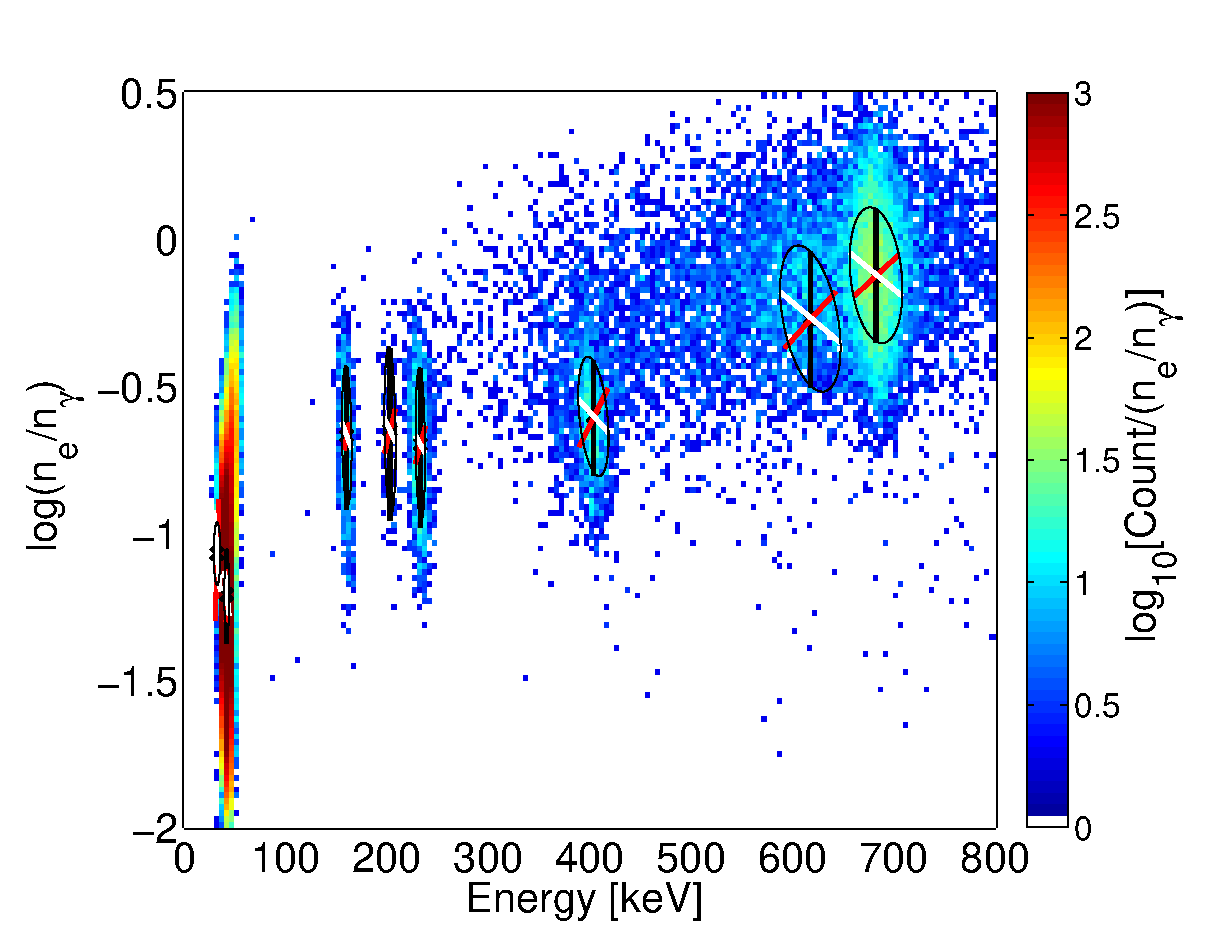
\includegraphics[width=120mm]{Figures/All_disc.eps}
\caption{Populations of calibration sources in discrimination space $\rm log\left(\frac{n_e}{n_\gamma}\right) $ vs. combined energy [$\rm keV_{ee}$]. The ovals represent the combination of $\rm \sigma R, \, \sigma n_{\gamma_{Det}}, \,\sigma n_{e_{Det}} $ in black, white, red respectively.}
\label{fig:E_dis}
\end{figure}

 \begin{figure}[h!]\centering
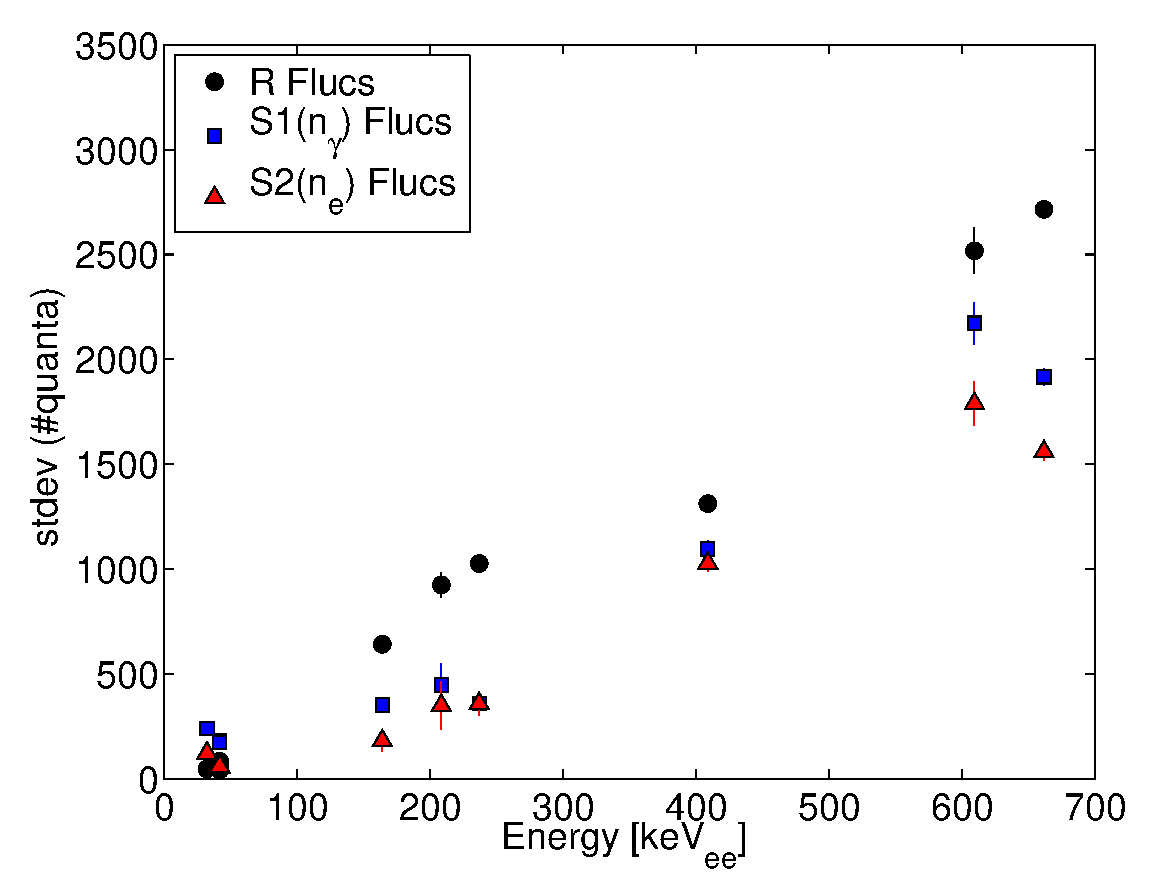
\includegraphics[width=80mm]{Figures/fluc_E.eps}
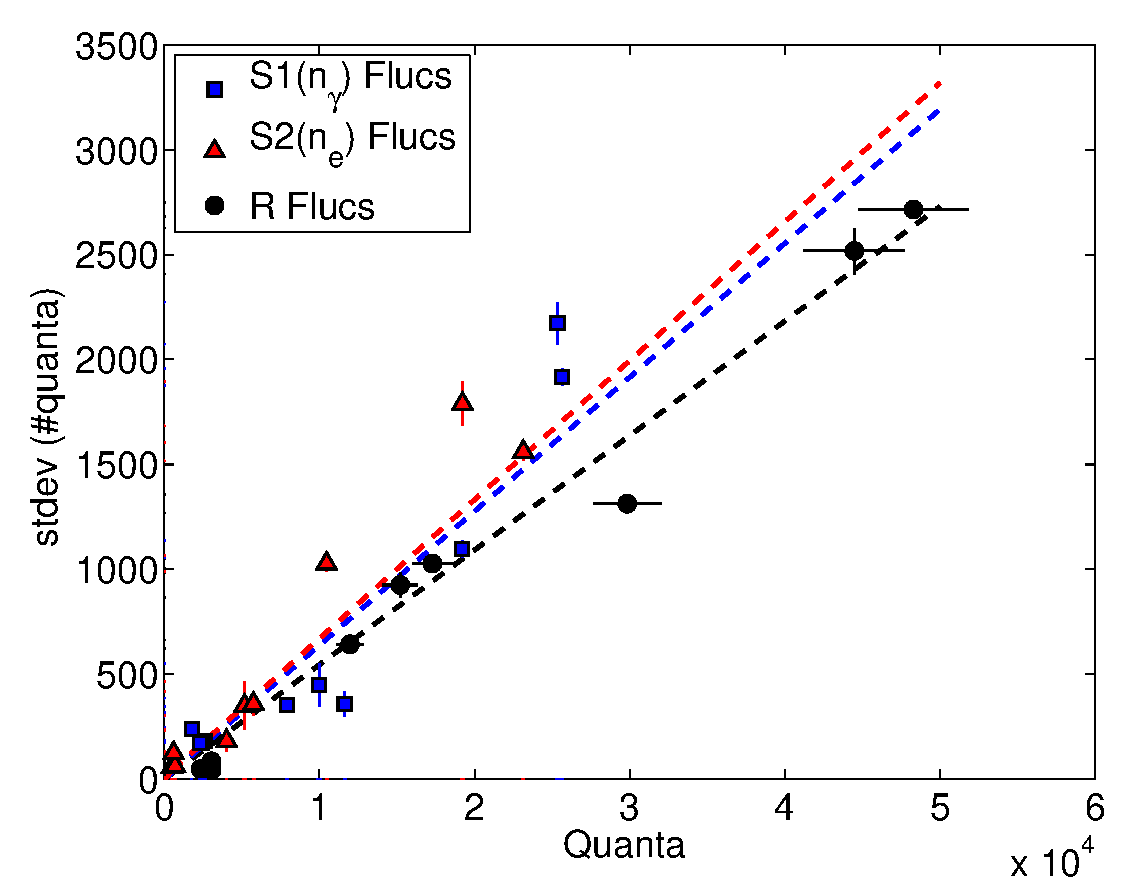
\includegraphics[width=80mm]{Figures/fluc_Q.eps}
\caption{Measured values of $\rm \sigma R, \, \sigma n_{\gamma_{Det}}, \,\sigma n_{e_{Det}} $ vs. Energy on the left and vs. Quanta on the right. Measured using sources listed in Table \ref{table:Cal_lines}. }
\label{fig:Flucs}
\end{figure}


\subsection{Measuring Recombination Fluctuations in Desecrate Energy Bins}
\label{Recomb_Mono}
The pervious subsection demonstrated the power of using a mono energetic source measure recombination fluctuations, equation  \ref{eq:Dahl}. In this section we present a method to decouple statistical variance from recombination fluctuations when confined to an energy bin of width $\rm \Delta_E$. The consideration of desecrate binning is crucial when dealing with a continual energy spectrum. Take the tritium beta spectrum as an example, we lose the ability to independently measure $\rm \sigma_{n_\gamma}^2$, $\rm \sigma_{n_e}^2$, $\rm \sigma_{E}^2 $ and are only left with a smear of $\rm n_\gamma$, $\rm n_e$, $\rm E $. However, there are two key pieces of information still left at our disposal. First, the combined energy can be reconstructed from global fits to g1 and g2, and even corrected for spectral shape and detector resolution (discussed later in section [link]). Second, we can calculate values of statistical variance for the light and charge channels as a function of energy, described in \ref{eq:SigStat},  \ref{eq:SigInst}. It will be shown in this section that having a priori knowledge of g1,g2 and the functional for of the statistical variance from detector resolution will be sufficient to measure recombination fluctuations for a continual energy spectrum binned in energy with width $\rm \Delta_E$.


We begin the treatment of binning with the the case of having a finite bin width around the central combined energy of a mono energetic source. First, we quantify the change in the statistical components of equation \ref{eq:SigR} when slicing out a bin in combined energy space. The slice in combined energy is illustrated for a toy model at quanta corresponding to that of the combined 41.6 keV $\rm^{83}Kr$ decay in Figure \ref{fig:Recomb}. All contribution from recombination fluctuations are included when slicing out a section of combined energy, illustrated in Figure \ref{fig:Recomb}. However, the slice contains only a reduced statistical component from both the light and charge signals, and in the limit that $\rm \Delta E$ goes to zero the statistical component of light and charge converge to a value defined as $\rm \chi_{stat}$ (where $\rm \chi$ is the measured $\rm \sigma$ in a bin of combined energy). To solve for the value of  $\rm \chi_{stat}$ we first calculate the slope induced by statistical variance in the number of photons vs. quanta and the complementary slope of electrons vs. quanta, defined as M and 1-M respectively.  The value of M depends on the magnitude of the statistical variances and is given in equation \ref{eq:Angle}. The sum of the two slopes must equal one as the sum of photons and electors make up combined energy.

 \begin{figure}[h!]\centering
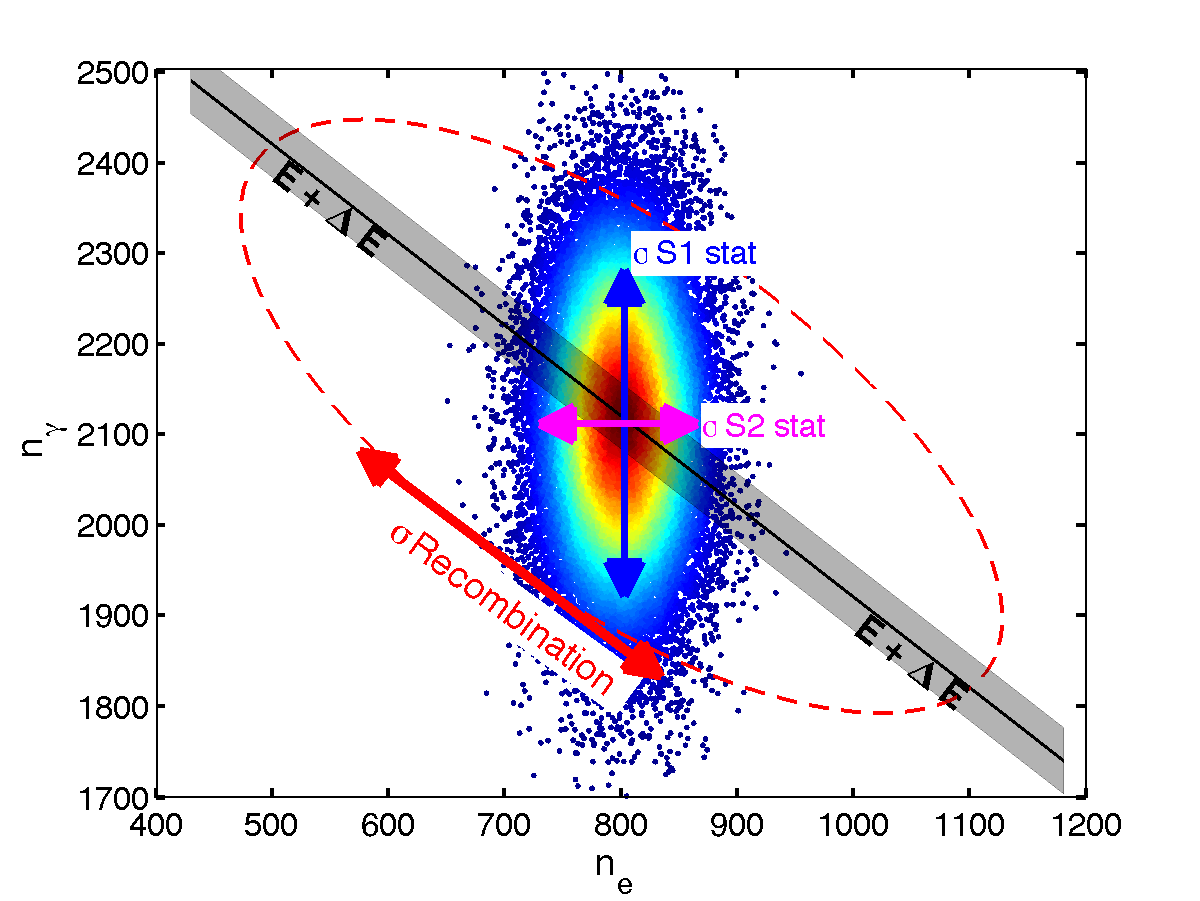
\includegraphics[width=150mm]{Figures/EX_Stat_Fano.png}
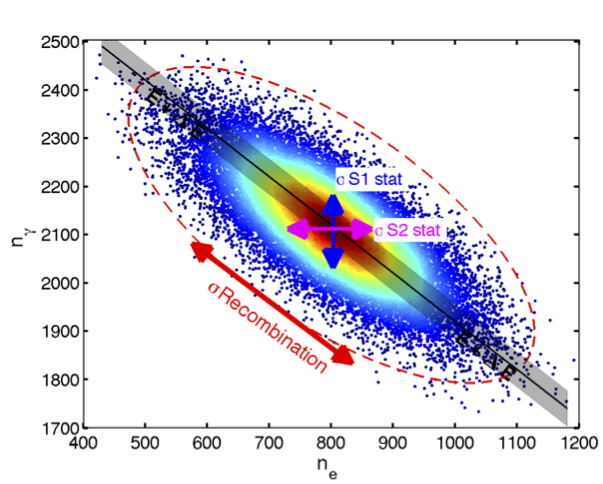
\includegraphics[width=80mm]{Figures/EX_R_Fano.png}
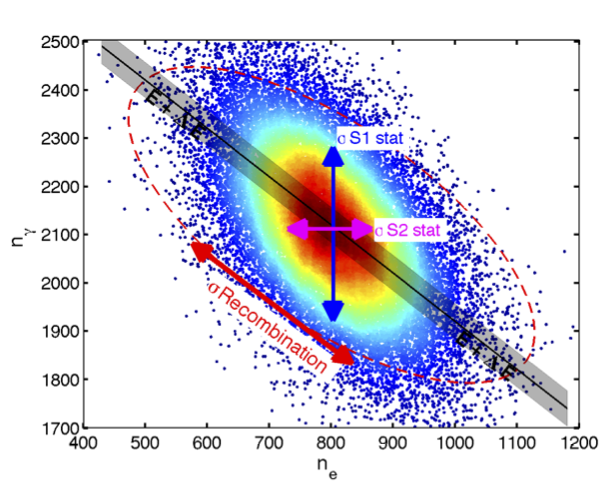
\includegraphics[width=80mm]{Figures/EX_Kr_Fano.png}
\caption{Top: Illustration of statistical variance, recombination fluctuations are set to 0. The spread in number of photons moves vertically and the spread in number of electrons moves horizontally. In black, a line of constant energy along the mean of combined energy with a width $\rm \Delta E$. Bottom left: Dominated by recombination fluctuations which move 45$^{\circ}$ to statistical variances. Bottom Right: Typical values for recombination and  S1, S2 Stat for $\rm Kr^{83}$. }
\label{fig:Recomb}
\end{figure}

\begin{equation}
\begin{split}
\rm M = tan(\theta_{n_{\gamma_{stat}}})=\frac{\sigma_{n_{\gamma_{stat}}}^2}{\sigma_{n_{\gamma_{stat}}}^2+ \sigma_{n_{\gamma_{stat}}}^2} \\
\rm 1-M = tan(\theta_{n_{e_{stat}}})=\frac{\sigma_{n_{e_{stat}}}^2}{\sigma_{n_{\gamma_{stat}}}^2+ \sigma_{n_{\gamma_{stat}}}^2} 
\label{eq:Angle}
\end{split}
\end{equation}


With the slope between combined energy and $\rm \sigma_{n_{\gamma_{stat}}}$ and between energy and $\rm \sigma_{n_{e_{stat}}}$ defined in equation \ref{eq:Angle} the value of the shared statistical uncertainty in combined energy space can be determined. We first treat the case of $\rm \Delta E$ = 0 in equation \ref{eq:SigCE}.

\begin{equation}
\rm \chi_{stat}^2= M^2\sigma_{n_{e_{stat}}}^2 + (1-M)^2\sigma_{n_{\gamma_{stat}}}^2
\label{eq:SigCE}
\end{equation}


The variable $\rm \chi$ is used to represent the observed $\rm \sigma$ when dealing in bins of combined energy. Let's briefly consider the implication of equation \ref{eq:SigCE}. For the case of $\rm \sigma_{n_{e_{stat}}}^2 = \sigma_{n_{\gamma_{stat}}}^2$, M=0.5, resulting in $\rm \sigma_{n_{e_{stat}}}^2=\sigma_{n_{\gamma_{stat}}}^2= \chi_{stat}^2$. This case can be thought of as sweeping out equal variance from the statistical population which would for a circle as illustrated in Figure \ref{fig:Recomb}. For the case of $\rm \sigma_{n_{e_{stat}}}^2 \neq \sigma_{n_{\gamma_{stat}}}^2$ the observed statistical variance in a slice of combined energy will become less than the variance of the best channel. Specifically for the LUX detector the implication of equation \ref{eq:SigCE} is that the statistical variance measured in a slice of combined energy will collapse to less than that of the S2 statistical uncertainty, as bin width $\rm \Delta_E$ goes to zero.


To complete the treatment of binned energy in this section we now add the final piece to the observed statistical variance, the contribution from the bin width $\rm \Delta_E$. The residual variance arrises from rotating the population of 2D gaussian about the bin center, the rotation having a slope of M or (1-M) as given in equation \ref{eq:Angle}. 


\begin{equation}
\begin{split}
\rm \chi_{n_{\gamma_{stat}}}^2= \chi_{stat}^2 + \frac{(MW\Delta_E)^2}{12}\\
\rm \chi_{n_{e_{stat}}}^2= \chi_{stat}^2 + \frac{((1-M)W\Delta_E)^2}{12}\\
\label{eq:SigCE_2}
\end{split}
\end{equation}



Were $\chi^2$ is defined in \ref{eq:SigCE}, M is given in equation \ref{eq:Angle}, W is the work function in [quanta/keV], $\rm \Delta_E$ is a bin of energy [keV], the normalization of 12 arrises from the second moment of a rotated line about its center. The total observed variance, $\rm \chi^2$, in the number of photons and electrons considering a bin of combined energy can now be determined transforming equation \ref{eq:SigR} to \ref{eq:Sig_total_CE}.

%%.... this equation holds for the standard deviation of a uniform distribution
 
\begin{equation}
\begin{split}
\rm \chi_{n_\gamma}^2 = \sigma_{n_{ex}}^2 + n_iF(r)^2 + \sigma_{r}^2 n_i^2 + \chi_{n_{\gamma_{stat}}}^2 \\
\rm \chi_{n_e}^2  = n_iF(1-r)^2 + \sigma_{r}^2 n_i^2 + \chi_{n_{e_{stat}}}^2
\label{eq:Sig_total_CE}
\end{split}
\end{equation}


In equation \ref{eq:Sig_total_CE} we have defined the observed spread in quanta $\rm \chi$ for $\rm n_\gamma, n_e$ when working with bins of combined energy. In the limit that F, $\rm \sigma_{n_{ex}}^2$ and $\rm \Delta_E$ go to zero the observed variance in number of photons and electrons ($\rm \chi_{n_\gamma}$ and $\rm \chi_{n_e}$) are related to the size of recombination fluctuations in a given combined energy bin, equation \ref{eq:SigR_CE_lim}. Where $\rm \sigma R$ is in units of quanta, $\rm \sigma_R = n_i\sigma_r$.

\begin{equation}
\begin{split}
\rm \sigma_{R_\gamma}^2 = \chi_{n_\gamma}^2 - \chi_{n_{\gamma_{stat}}}^2  \\
\rm \sigma_{R_e}^2 = \chi_{n_e}^2 - \chi_{n_{e_{stat}}}^2
\label{eq:SigR_CE_lim}
\end{split}
\end{equation}

We have arrived at the conclusion of this section, armed with equation \ref{eq:SigR_CE_lim} we now have two methods for determining the size of recombination fluctuations, $\rm\sigma_{R}^2$ where the subscript $\rm \gamma$ or e is used to represent the channel of quanta used for the calculation. Either the observed variance in the light and charge channel can be used to measure the size of recombination fluctuation in a bin of energy. Any discrepancy between the two methods has implications which are discussed in the following subsection.

\subsection{Measuring the Fano Factor in Bins of Energy}


There are three terms in equation \ref{eq:Sig_total_CE} that give rise to an asymmetry between the observed variance $\rm \chi_{n_\gamma}^2$ and $\rm \chi_{n_e}^2$. The small difference in the statistical component can be solved for exactly leaving just the Fano factor F and $\rm \sigma_{n_{ex}}^2$. By taking the difference of $\rm \chi_{n_\gamma}^2$ and $\rm \chi_{n_e}^2$ the variance from recombination drops out along with most of the statistical variance leaving only the Fano factor and the variance in number of exitons, given in equation \ref{eq:Sig_total_CE}.

\begin{equation}
\rm \chi_{n_\gamma}^2 - \chi_{n_e}^2 = \sigma_{n_{ex}}^2 + n_iF(2r-1) + \delta_{stat}
\label{eq:Diff_X}
\end{equation}

F is the Fano factor, equation \ref{eq:Energy_2}, $\rm \sigma_{n_{ex}}^2$ is the variance of the number of exitons produced and r is the recombination fraction, equation \ref{eq:Quanta}. The value of $\delta_{stat}$ is the small residual depending on the bin width $\rm \Delta_E$, equation \ref{eq:Residual_Stat}.

\begin{equation}
\rm \delta_{stat}= \chi_{n_{\gamma_{stat}}}^2 - \chi_{n_{e_{stat}}}^2 = \frac{(2M-1)(W\Delta_E)^2}{12}\\
\label{eq:Residual_Stat}
\end{equation}

Consider the case such that variance in the number of exitons $\rm \sigma_{n_{ex}}^2$ is much less than the contribution from the Fano factor. In such a regime we can solve for the Fano factor, potentially energy dependent, from equations \ref{eq:Diff_X} and \ref{eq:Residual_Stat}.

\begin{equation}
\rm F(E)=\frac{\chi_{n_\gamma}^2 - \chi_{n_e}^2 - \delta_{stat}}{n_i(2r-1)}
\begin{cases} \rm r \neq \frac{1}{2}\\
\end{cases}
\label{eq:Fano}
\end{equation}

There is an underlying subtlety to equation \ref{eq:Fano}. Remarkably, in the limit that $\rm \Delta_E$ goes to zero the Fano factor can be extracted with minimal knowledge of intrinsic detector statistical variance. Further, when the statistical variance of S1 and S2 are identical the value of M (equation \ref{eq:Residual_Stat}) will be 0.5. In that special case no knowledge of the statistical variance is needed to measure the Fano factor. 


When $ \rm r = \frac{1}{2}$ the coefficient in front of the Fano factor becomes zero in equation \ref{eq:Diff_X}. At this value an equal contribution from the Fano factor goes into the variance $\rm \chi^2$ of photons and electrons, allowing for the smaller value of $\rm \sigma_{ex}^2$ to be extracted. 

\begin{equation}
\rm \sigma_{n_{ex}}^2=\chi_{n_\gamma}^2 - \chi_{n_e}^2 - \delta_{stat}
\begin{cases} \rm r= \frac{1}{2} || \sigma_{n_{ex}}^2 > > n_iF(2r-1)\\
\end{cases}
\label{eq:SigmaEx}
\end{equation}

Equation \ref{eq:SigmaEx} is also valid in the case that $\rm \sigma_{n_{ex}}^2$ is much larger than the contribution form the Fano factor. This happens to be true when dealing with the time dependent light yield of $\rm ^{83m}Kr$, this topic will be explored in the next section.




\subsection{Application to $\rm^{83}Kr$}


...Knowing the statistical uncertainties from a simulated Kr data set of 400,000 events with 100 trials. Using equation \ref{eq:SigR_CE_lim} we find good agreement between the method described in equation \ref{eq:Dahl} and the recombination fluctuation calculated from the charge channel ($\rm \sigma_{R_e}$). There is a clear systematic offset outside the bounds of the respective uncertainties between the light and charge channels, this indicates that the additional contribution from $\rm \sigma_{n_{ex}}$ is on the order of 34 quanta. This value is consistent with the enhanced time dependent light yield from the second 9.4 keV decay of $\rm ^{83m}Kr$, for which the mean shifts by up to 10 Phe in S1 (or 70 Photons) with a timing separation cut of 1000 ns. [ Add Light Yield vs. dT plot here]. 

\begin{table}[h!]
\begin{center}
\begin{tabular}{|c|c|c|c|c|c|}
\hline
$\rm \Delta_E$ [keV] & Count & $\rm \sigma(\chi_{n_{\gamma}}^2-\chi_{n_{\gamma_{stat}}}^2)$ & $\rm \sigma(\chi_{n_{e}}^2-\chi_{n_{e_{stat}}}^2)$  & $\rm \sigma(\chi_{n_\gamma}^2 - \chi_{n_e}^2 - \delta_{stat})$\\ \hline
0.05 	& 3309 	& 114.1  	&	114.3	& 2.5	 \\ \hline
0.1 	& 6612  	& 84.5 	& 	84.5	& 3.4	 \\ \hline
0.2 	& 13230  	& 55.8 	& 	55.7	& 4.2	 \\ \hline
0.25 	& 16533 	& 53.4		&	53.5  	& 5.0	 \\ \hline
0.5		& 33011 	& 32.9  	&	32.6	& 7.6	 \\ \hline
\end{tabular}
\caption{Values for the standard deviation of the observed value of $\rm \sigma_R^2$ from $\rm n_\gamma$ and $\rm n_e$ along with the standard deviation of the difference, for a simulated $\rm^{83m}Kr$ decay with recombination set to zero.  Note, since the two methods for determining $\rm \sigma_R^2$  are correlated the standard deviation of the measured difference is small leading to an improved error when calculating the Fano factor or $\rm \sigma_{n_{ex}}^2$.}
\label{table:Simulated_Sigmas_R_0}
\end{center}
\end{table}

\begin{table}[h!]
\begin{center}
\begin{tabular}{|c|c|c|c|c|c|}
\hline
$\rm \Delta_E$ [keV] & Count & $\rm \sigma(\chi_{n_{\gamma}}^2-\chi_{n_{\gamma_{stat}}}^2)$ & $\rm \sigma(\chi_{n_{e}}^2-\chi_{n_{e_{stat}}}^2)$  & $\rm \sigma(\chi_{n_\gamma}^2 - \chi_{n_e}^2 - \delta_{stat})$\\ \hline
0.05 	& 3316 	& 327.0  	&	326.3	& 4.7	 \\ \hline
0.1 	& 6623  	& 257.3 	& 	257.2	& 5.9	 \\ \hline
0.2 	& 13237  	& 196.2 	& 	196.8	& 9.0	 \\ \hline
0.25 	& 16539 	& 180.3	&	180.7  	& 11.1	 \\ \hline
0.5		& 33019 	& 114.1  	&	117.0	& 16.2	 \\ \hline
\end{tabular}
\caption{Values for the standard deviation of the observed value of $\rm \sigma_R^2$ from $\rm n_\gamma$ and $\rm n_e$ along with the standard deviation of the difference, for a simulated $\rm^{83m}Kr$ decay with recombination set to 100 quanta.  Note, since the two methods for determining $\rm \sigma_R^2$  are correlated the standard deviation of the measured difference is small leading to an improved error when calculating the Fano factor or $\rm \sigma_{n_{ex}}^2$.}
\label{table:Simulated_Sigmas_R_100}
\end{center}
\end{table}



\begin{table}[h!]
\begin{center}
\begin{tabular}{|c||c|c|c|c|c|}
\hline
$\rm \sigma_R$ Dahl \ref{eq:Dahl} & $\rm \Delta_E$ & Count & $\rm \sigma_{R_\gamma}=\sqrt{\chi_{n_{\gamma}}^2-\chi_{n_{\gamma_{stat}}}^2}$ & $\rm \sigma_{R_e}= \sqrt{\chi_{n_{e}}^2-\chi_{n_{e_{stat}}}^2}$  & $\rm \sigma_{n_{ex}}=\sqrt{\chi_{n_\gamma}^2 - \chi_{n_e}^2 - \delta_{stat}}$\\ 
(Quanta) & (keV) & & (Quanta) & (Quanta) & (Quanta) \\ \hline
94.3 $\pm$ 0.1	& 0.05 		& 3383 	& 97.7 $\pm$ 1.5	 	&	92.0 $\pm$ 1.6	& 33.1 $\pm$ 0.1	 \\ \hline
					& 0.1 		& 6876  	& 97.2 $\pm$ 1.2		& 	91.4 $\pm$ 1.3	& 33.0 $\pm$ 0.1	 \\ \hline
					& 0.2 		&13583  	& 97.1 $\pm$ 0.9  		& 	91.4 $\pm$ 1.0	& 32.9 $\pm$ 0.1	 \\ \hline
					& 0.25 		&16955 	& 97.3 $\pm$ 0.9		&	91.8 $\pm$ 0.9  	& 32.4 $\pm$ 0.2	 \\ \hline
					& 0.5		& 33721 	& 97.6  $\pm$ 0.5		&	91.1 $\pm$ 0.6	& 32.9	$\pm$ 0.2 \\ \hline
\end{tabular}
\caption{Values for the standard deviation of the observed value of $\rm \sigma_R^2$ from $\rm n_\gamma$ and $\rm n_e$ along with the standard deviation of the difference, for a $\rm^{83m}Kr$ data set. }% add note about exitons
\label{table:R_Kr}
\end{center}
\end{table}


Table \ref{table:R_Kr} shows the comparison of recombination fluctuations when calculated in binned energy space vs. the conventional method for a $\rm ^{83m}Kr$ data set. $\rm \sigma_{R_{e}}$ is immune to time dependence of exiton production and predicts the correct value of recombination to within 3\%. The accuracy helps us build confidence that the statistical components of the detector are modeled well enough to measure recombination fluctuation to within 3\%. The ability to actually measure $\rm \sigma_{n_{ex}}$ from the additional contribution in $\rm \sigma_{R_{\gamma}}$ demonstrates the power of using binned combined energy. Any observed difference between the two channels  can only be from either the Fano factor or spread in exiton production, see Table \ref{table:Simulated_Sigmas_R_100} and \ref{table:Simulated_Sigmas_R_0} and equation \ref{eq:Sig_total_CE}.The next step will be to apply the method on the Tritium data.


\subsection{Application to Tritium Data (Will go after Section 4 where the Smearing Model is discussed)}

After applying the Smearing Model of Section 4 we apply the method described in this section to extract recombination fluctuations form the tritium data.

In this subsection we test method outlined in section \ref{Recomb_Mono} for dealing in bins of combined energy when applied to the tritium beta spectrum. To first order the treatment of the continuous spectrum is identical to that outlined for the mono energetic source. Figure \ref{fig:T_Stat} shows a tritium spectrum smeared with only intrinsic detector resolution, the figure is analogous to Figure \ref{fig:Recomb}. As the bin size around a value of combined energy is squeezed to zero the statistical variance in the number of photons and electrons converge, the value is given by equation \ref{eq:SigCE_2}. Whereas, regardless of bin size recombination fluctuations remain since they move along lines of constant energy. 
The tritium spectral shape may cause a perturbation to the analytic solution for observed variance $\rm \chi^2$, equation \ref{eq:SigCE_2}. To observe any discrepancy we test the analytic solution against the observed variance of a simulated tritium spectrum. Figure \ref{fig:T_Var} shows the result of the analytic solution vs. the observed variance in several bin widths. The analytic solution is sufficient to first order, we ignore second order corrections in this analysis. [add table showing the tiny difference in variance]. 

\begin{figure}[h!]\centering
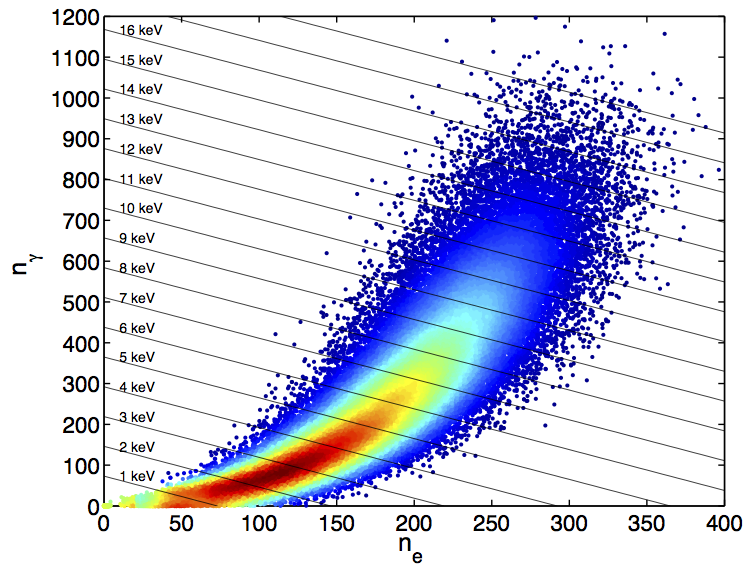
\includegraphics[width=150mm]{Figures/EX_T_Fano.png}
\caption{Illustration of statistical variance for the tritium beta spectrum, recombination fluctuations are set to 0. This plot is analogous to Figure \ref{fig:Recomb} which illustrates the case for the mono energetic $\rm ^{83m}Kr$ decay. Recombination fluctuation move along lines of constant energy, S1 statistical fluctuation move vertically and S2 statistical fluctuations move horizontally. }
\label{fig:T_Stat}
\end{figure}


\begin{figure}[h!]\centering
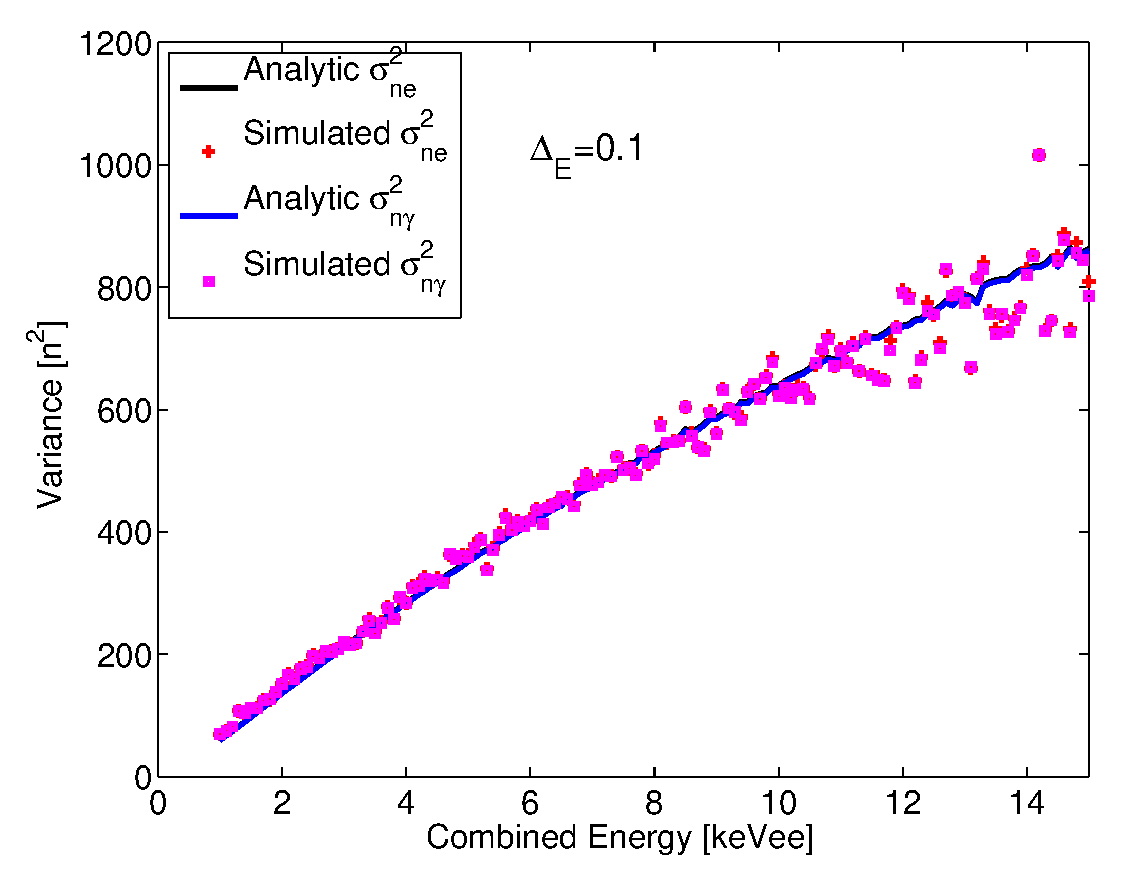
\includegraphics[width=80mm]{Figures/SIM_stat_T_10Fano.eps}
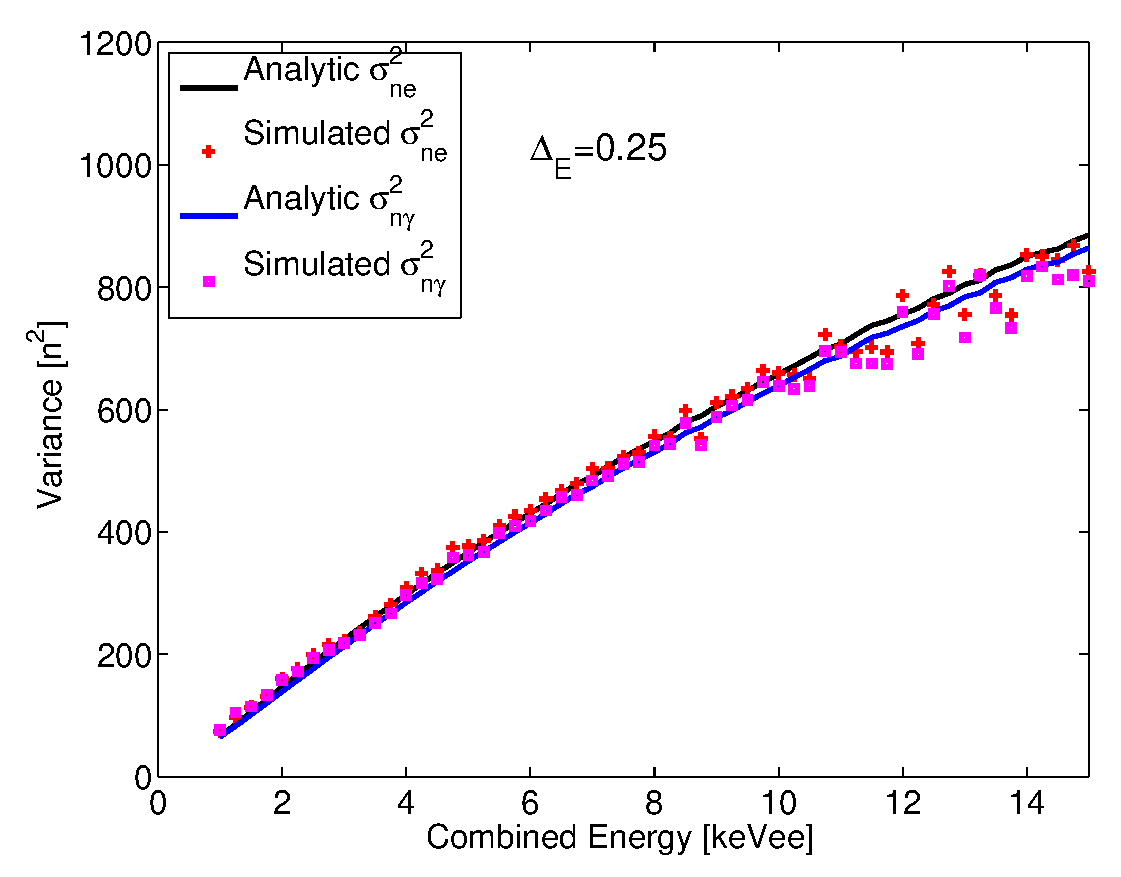
\includegraphics[width=80mm]{Figures/SIM_stat_T_25Fano.eps}
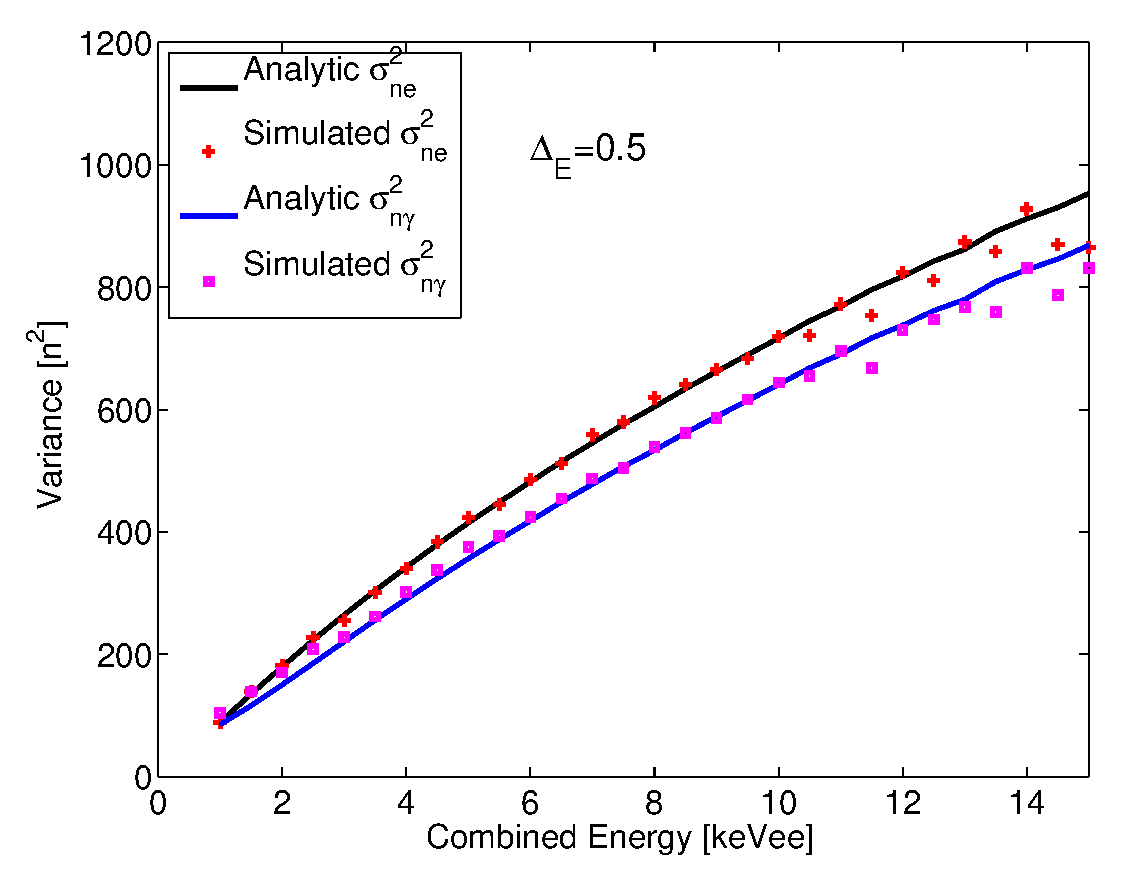
\includegraphics[width=80mm]{Figures/SIM_stat_T_50Fano.eps}
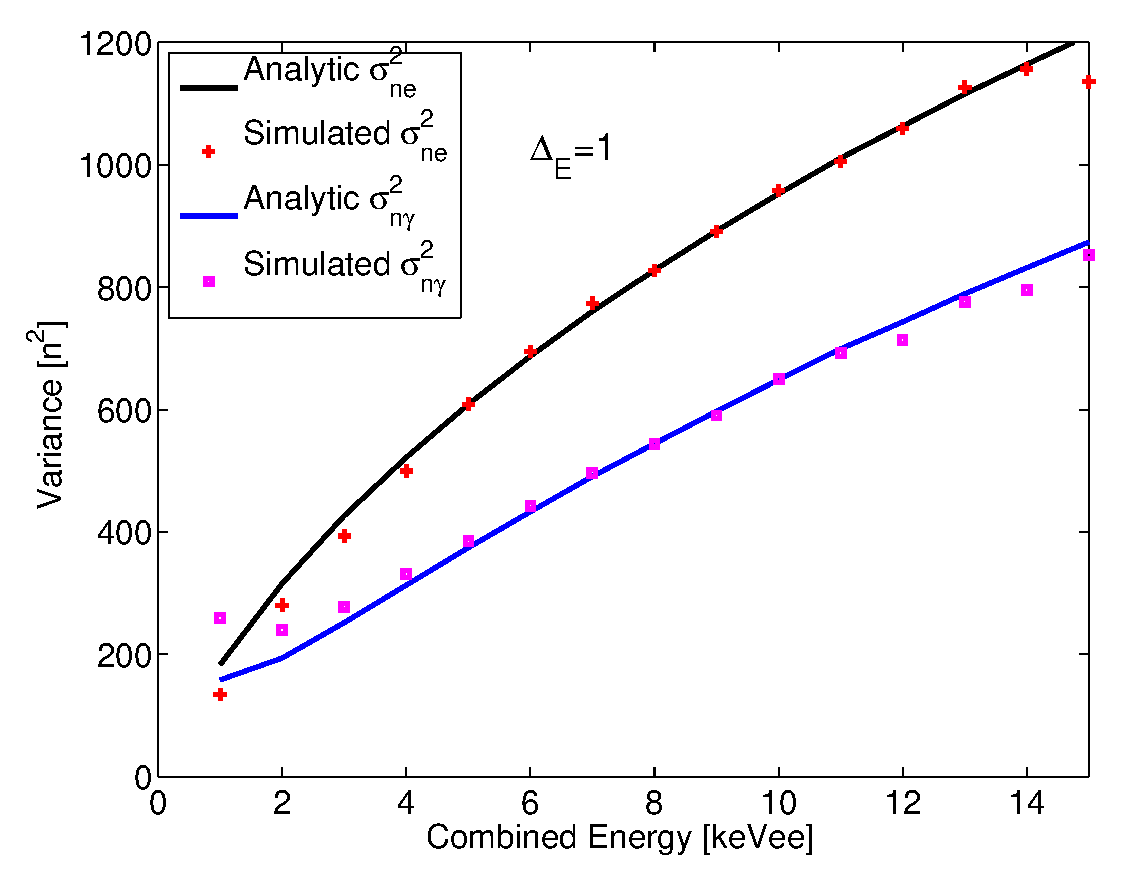
\includegraphics[width=80mm]{Figures/SIM_stat_T_100Fano.eps}
\caption{The analytic variance calculated from equation \ref{eq:SigCE_2} vs. the observed statistical variance for a simulated tritium spectrum at several bin widths ($\Delta_E$. }
\label{fig:T_Var}
\end{figure}

After correcting observables for the tritium beta spectral shape (discussed in Section 4) we will be ready to use the tools of this section to decouple detector resolution and measure recombination fluctuations from the tritium data.... Even set a limit on the Fano factor while we're at it.


The first step is to solve for the value of $\rm \sigma_R$ (recombination fluctuation) that needs to be input into the smearing model, the statistical part from detector resolution remains fixed. Figure \ref{fig:R_T} show the optimal value of $\rm \sigma_R$ being extracted from the tritium data, starting with an initial guess based on the recombination fluctuation measured from the $\rm^{83m}Kr$ data.

\begin{figure}[h!]\centering
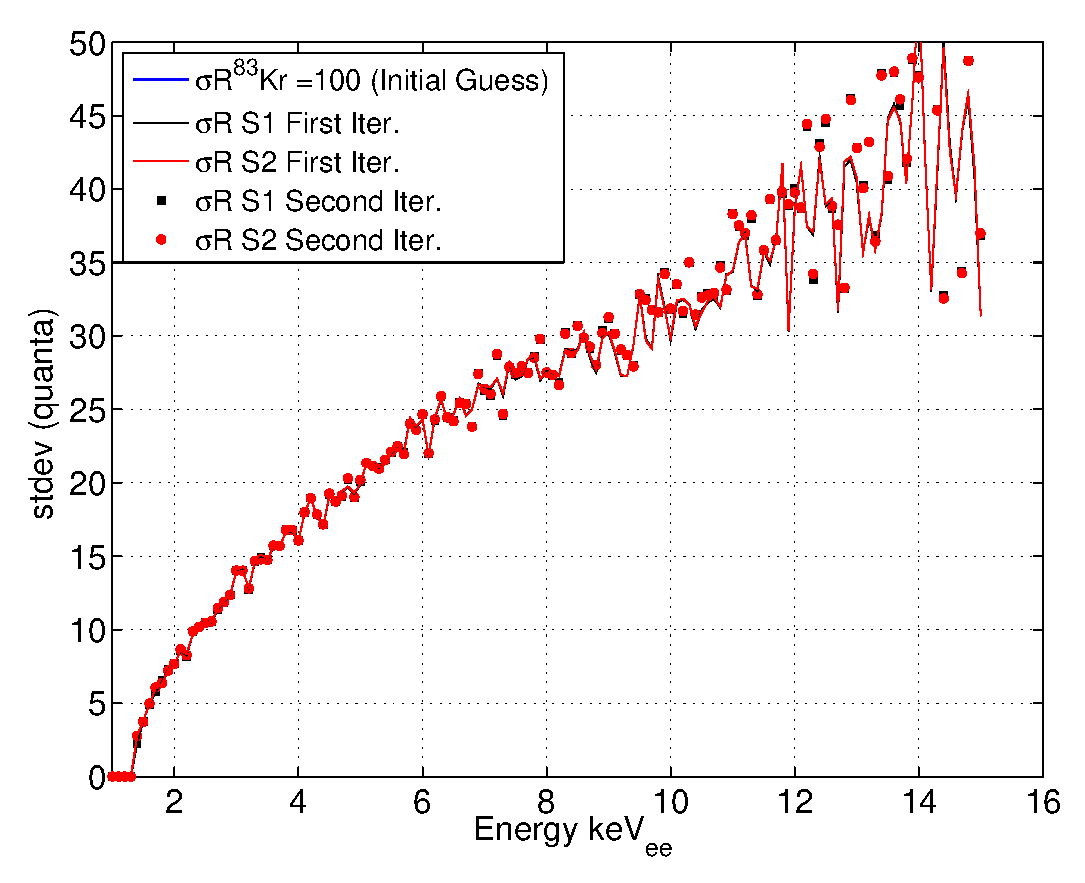
\includegraphics[width=100mm]{Figures/R_.eps}
\caption{Extracting $\rm \sigma_R$ from the tritium data. }
\label{fig:R_T}
\end{figure}


\begin{figure}[h!]\centering
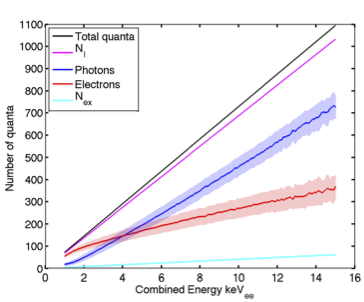
\includegraphics[width=80mm]{Figures/quanta_Fano.png}
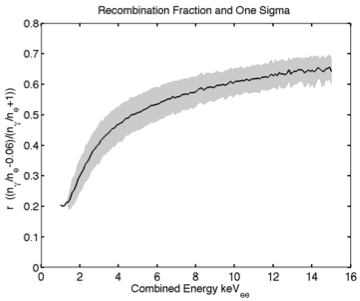
\includegraphics[width=80mm]{Figures/R_Fano.png}
\caption{Recombination fraction and its corresponding one sigma. $\rm \sigma_r=\sigma_R/n_{ions}$ .}
\label{fig:R_T}
\end{figure}


\begin{figure}[h!]\centering
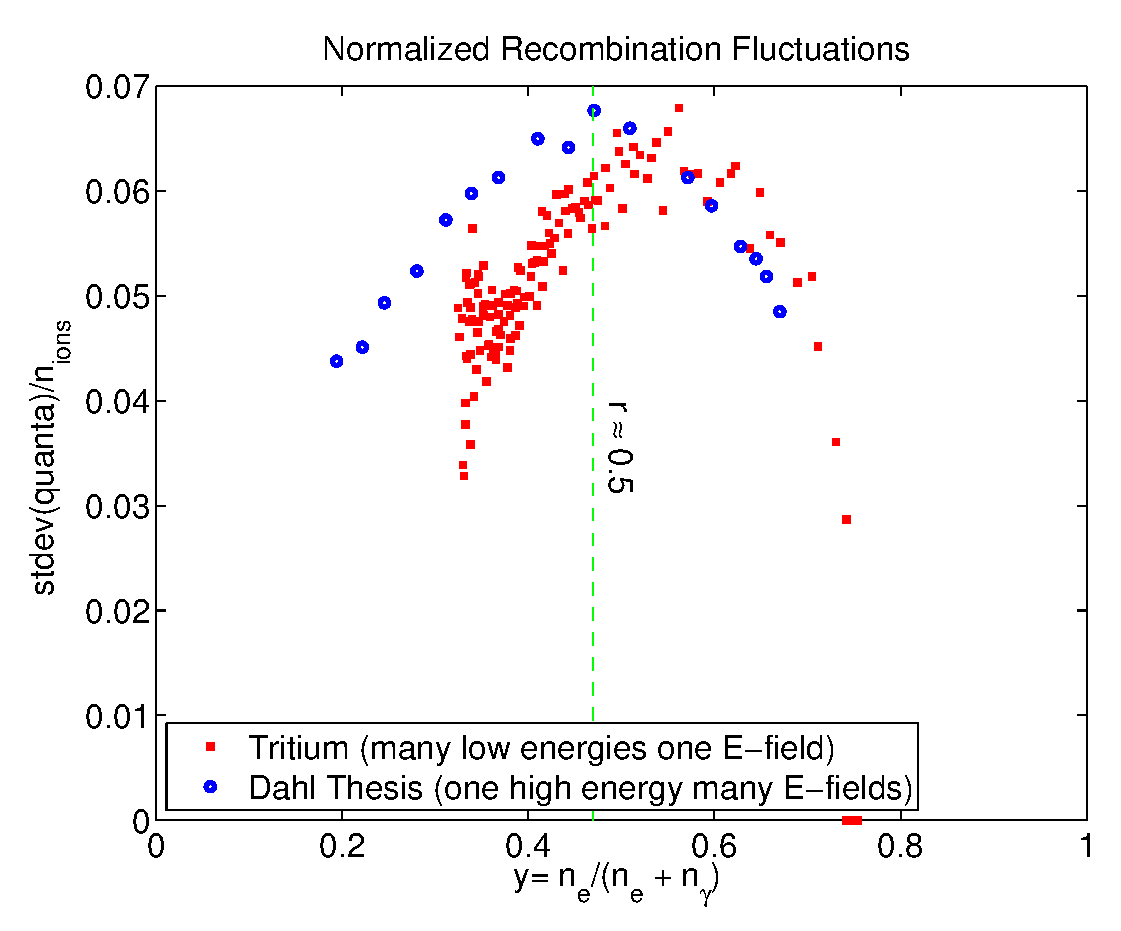
\includegraphics[width=120mm]{Figures/Dahl_fig_Fano.eps}
\caption{Recombination fraction. }
\label{fig:R_T}
\end{figure}

\begin{figure}[h!]\centering
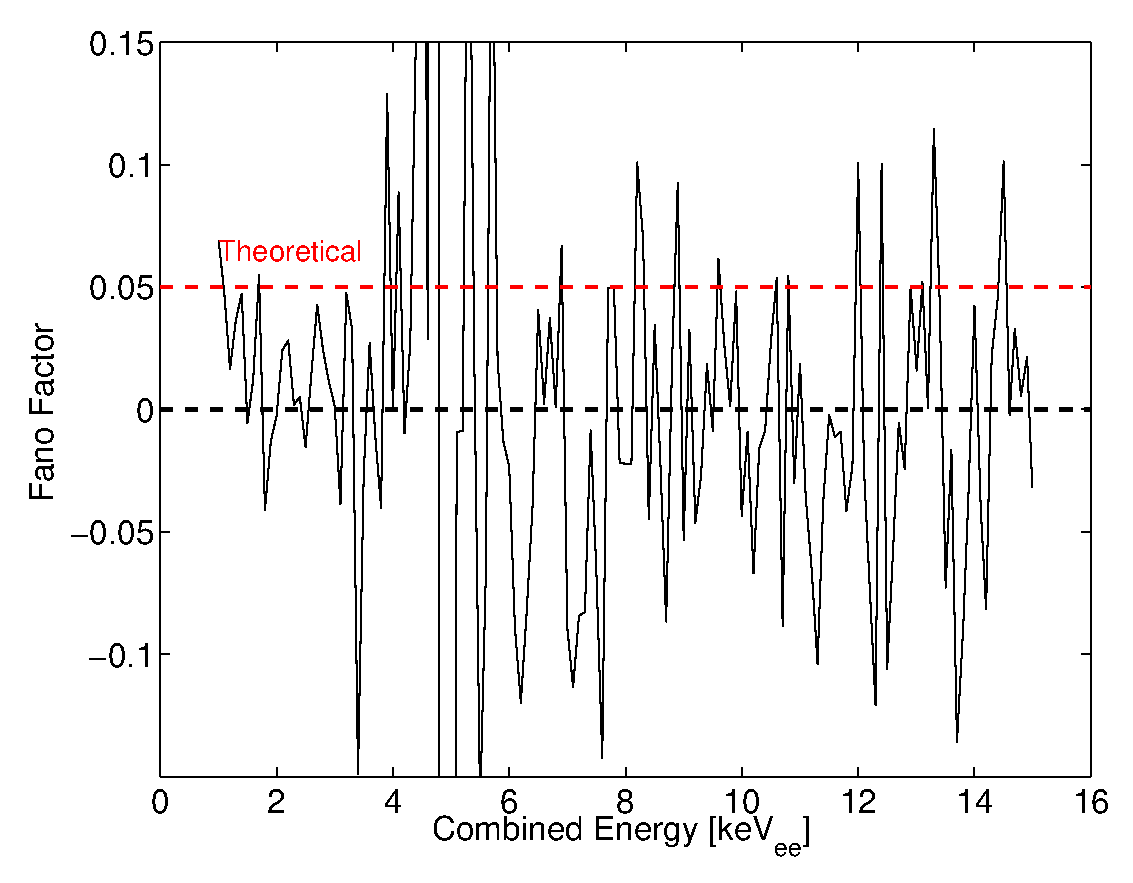
\includegraphics[width=100mm]{Figures/Fano_T_Fano.eps}
\caption{Fano factor extracted from tritium data. Calculated from difference between $\rm \sigma_{R_\gamma}$ and $\rm \sigma_{R_e}$, see equation \ref{eq:Fano}. We find F = -0.01 $\pm$ 0.07, with the theoretical value in liquid xenon being F=0.05. \cite{FanoTheoretical}. }
\label{fig:R_T}
\end{figure}



%% Show plot similar to F(E)
\newpage
\section{Correcting the Tritium Spectral Shape for Finite Resolution (Out of Date)}

The distribution of tritium events convolved with finite resolution for S1 (scintillation) and S2 (ionization) causes the observed mean to shift from the actual mean. The shift is non trivial and depends on the spectral shape and the resolution. A large negative derivative of the spectral shape will tend to pull the observed spectrum to lower values, and the functional form of the of resolution will also shift the spectrum. Figure \ref{fig:exp_int} and equations \ref{eq:2},\ref{eq:4} demonstrate a simple model to solve for the relation between observed mean and actual mean. Take for example a linearly declining distribution, starting with infinite detector resolution we set up bins of width $\rm \Delta x$. To account for finite energy resolution we distribute the counts in each rectangular bin into Gaussians centered at $\rm \mu_i$, with a spread of $\sigma_i$, and normalized to the area of the bin $\rm N_i \times \Delta x $ with amplitude $\rm c_i$. Each rectangular bin(i) can be written as a Gaussian G(i): \\ 
\begin{multline}
\\ \rm c_i=\frac{N_i \times \Delta x}{\sigma_i\sqrt{2\pi}} \\
\rm G_{i}(x) = c_i \times exp\left(\frac{-(x-\mu_i)^2}{2\sigma_i^2}\right)\\
\label{eq:1}
\end{multline}


Where $\rm N_i$ is the count in the $\rm i^{th}$ bin, $\rm \Delta x$ is the bin width, $\rm \mu_i$ is the bin center and $\rm \sigma_i$ is the resolution at the $\rm i^{th}$ bin. Figure \ref{fig:exp_int} show the application of equation \ref{eq:1} to a linear energy distribution with a $\rm \sqrt{E}$ dependent $\sigma$. The observed distribution is the sum of the Gaussians, shown in red.

 \begin{figure}[h!]\centering
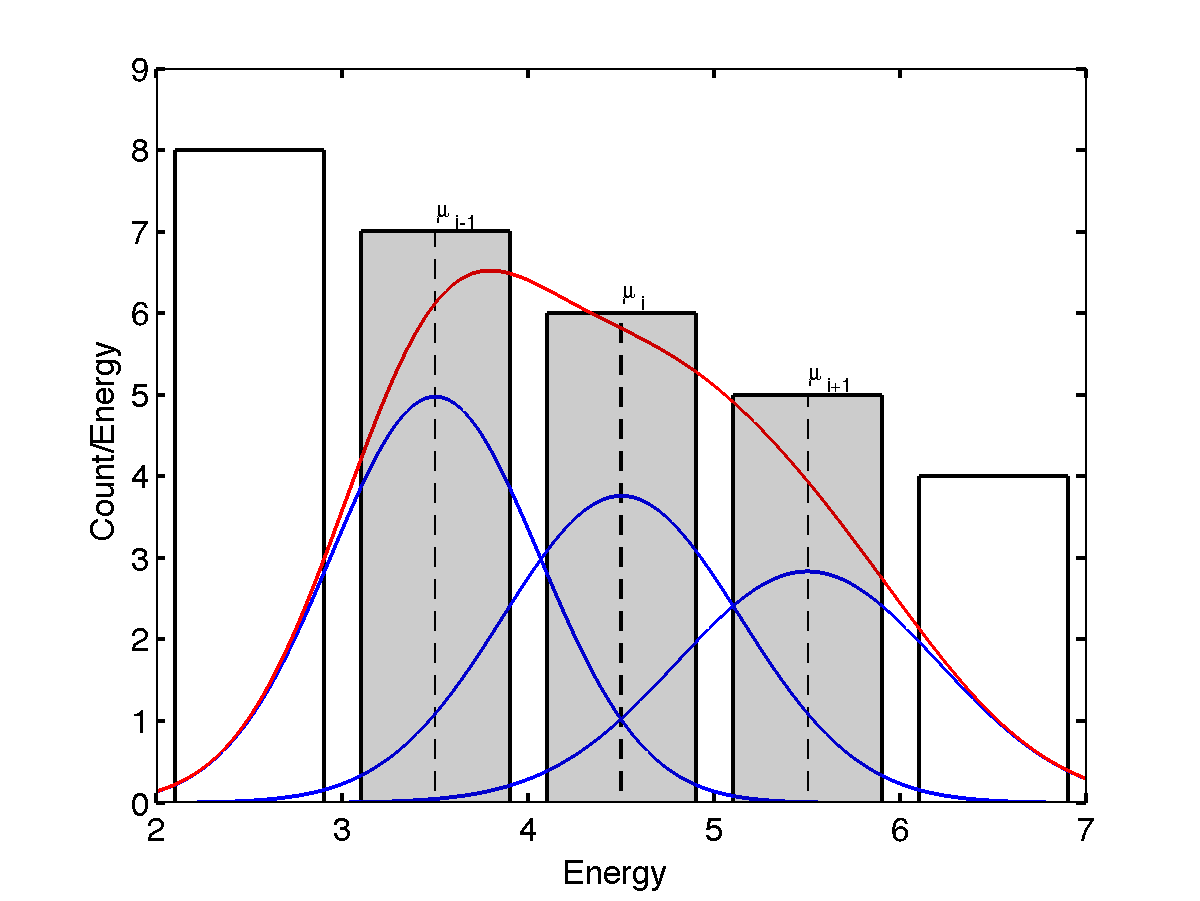
\includegraphics[width=130mm]{Figures/example_integral}
\caption{}
\label{fig:exp_int}
\end{figure}


\subsection{Calculating the Observed Energy}

After modeling the finite resolution with Gaussians the mean observed at each bin can be calculated from the overlap of all bins weighted by the corresponding means. We can write the observed mean in the $\rm i^{th}$ bin, $\nu_i$, in terms of the bin centers $\mu$ and overlapping areas of all bins using equation \ref{eq:1}:
%\begin{center}
\begin{equation}
\Large \nu_i = \frac{\mathlarger{\sum}\limits_{j=1}^{n}\ \mu_j\mathlarger{\int}\limits_{\mathsmaller{\mu_i-\frac{\Delta x}{2}}}^{\mathsmaller{\mu_i+\frac{\Delta x}{2}}} G_{j}(x)\,\mathrm{d}x} 
{\mathlarger{\sum}\limits_{j=1}^{n} \ \mathlarger{\int}\limits_{\mathsmaller{\mu_i-\frac{\Delta x}{2}}}^{\mathsmaller{\mu_i+\frac{\Delta x}{2}}} G_{j}(x)\,\mathrm{d}x}  
\label{eq:2}
\end{equation}
%\end{center}

Equation \ref{eq:2} can be solved in terms of error function and complimentary error function, first we will generalize a formula to solve for the overlapping area from the $\rm j^{th}$ bin into the $\rm i^{th}$ bin. 
\begin{equation}
%\rm A_i = c_i \ erf\left(\frac{\Delta x}{\sigma_i\sqrt{2}}\right) + \sum\limits_{n\neq i}^{} \frac{c_n}{2} erfc\left(\frac{|\mu_n-\mu_i| - \frac{\Delta x}{2}}{\sigma _n\sqrt{2}} \right) - 
%\sum\limits_{n\neq i}^{} \frac{c_n}{2} erfc\left(\frac{|\mu_n-\mu_i| + \frac{\Delta x}{2}}{\sigma _n\sqrt{2}} \right) 
\Large \rm A_{i,j}=\mathlarger{\int}\limits_{\mathsmaller{\mu_i-\frac{\Delta x}{2}}}^{\mathsmaller{\mu_i+\frac{\Delta x}{2}}}\it G_{j}(x)\,\mathrm{d}x =
\begin{cases}\rm c_i \ erf\left(\frac{\Delta x}{\sigma_i\sqrt{2}}\right), & j=i  \\ \\
\rm \frac{c_j}{2} erfc\left(\frac{|\mu_j-\mu_i| - \frac{\Delta x}{2}}{\sigma _j\sqrt{2}} \right) - 
\rm \frac{c_j}{2} erfc\left(\frac{|\mu_j-\mu_i| + \frac{\Delta x}{2}}{\sigma _j\sqrt{2}} \right) , & j \neq i \end{cases}
\label{eq:3}
\end{equation}

As $\rm \mu$ approaches zero the Gaussian distribution of equation \ref{eq:1} begins to spill over into negative values, which in some cases may be unphysical. For instance, the Gaussian assumption leads to negative photons. We can chose to ignore this area or make the distribution more Poisson like by bouncing the Gaussian back at $\rm \mu = 0$. The formula for accounting for the area of the reflected Gaussian is described in \ref{eq:6}. Ultimately this assumption has little impact on the S1 and S2 analysis because the threshold cut off well before the zero interface is reached, but it does make the distributions more Poisson like near the zeroth bins. Equation \ref{eq:6} is the same as \ref{eq:3} with the bin center $\rm \mu_i$ mapped to $\rm -\mu_i$.

\begin{equation}
%\rm A_i = c_i \ erf\left(\frac{\Delta x}{\sigma_i\sqrt{2}}\right) + \sum\limits_{n\neq i}^{} \frac{c_n}{2} erfc\left(\frac{|\mu_n-\mu_i| - \frac{\Delta x}{2}}{\sigma _n\sqrt{2}} \right) - 
%\sum\limits_{n\neq i}^{} \frac{c_n}{2} erfc\left(\frac{|\mu_n-\mu_i| + \frac{\Delta x}{2}}{\sigma _n\sqrt{2}} \right) 
\rm B_{i,j}=
\rm \frac{c_j}{2} erfc\left(\frac{|\mu_j+\mu_i| - \frac{\Delta x}{2}}{\sigma _j\sqrt{2}} \right) - 
\rm \frac{c_j}{2} erfc\left(\frac{|\mu_j+\mu_i| + \frac{\Delta x}{2}}{\sigma _j\sqrt{2}} \right)
\label{eq:6}
\end{equation}

The error function and complementary error function are defined in equation \ref{eq:4} and the coefficient $\rm c_i$ is defined in equation \ref{eq:1}.
\begin{multline}
\\ \rm erf(x)=\frac{2}{\sqrt{\pi}} \times \int\limits_{0}^{x} exp(-t^2)\\
\rm erfc(x)=\frac{2}{\sqrt{\pi}} \times \int\limits_{x}^{\infty} exp(-t^2) = 1 - erf(x)\\
\label{eq:4}
\end{multline}

Finally, we solve for the observed mean in the $\rm i^{th}$ bin by summing all the Gaussian overlaps $\rm A_{i,j}$ + $\rm B_{i,j}$ (equations \ref{eq:3},\ref{eq:6}), weighting the overlapping area from each bin by the corresponding bin center $\rm \mu_j$. The result is shown in equation \ref{eq:5} and is equivalent to equation \ref{eq:2} when the area from the reflected Gaussian is not considered, $\rm B_{i,j}$=0.
\begin{equation}
\rm \Large \nu_i =  \frac{\sum\limits_{j=1}^{n}\mu_j\cdot (A_{i,j}+B_{i,j})}{\sum\limits_{j=1}^{n} (A_{i,j}+B_{i,j})}
\label{eq:5}
\end{equation}

\subsection{Smearing a Toy Spectrum}

To demonstrate the application of equation \ref{eq:5} we use it to smear a toy linearly decaying spectrum. By modifying the dependence of $\rm \sigma_i$ on $\rm \mu_i$ we can better understand the effects of the spectral shape and the functional for of the resolution.

Figure \ref{fig:Toy_Linear} shows the effect of the finite resolution on a linearly decaying spectral shape. Using a constant resolution $\rm \sigma$ the observed mean, when accounting for finite resolution, shifts down due to the spectral shape. In the case with $\rm \sigma_i \sim \sqrt{\mu_i} $ the observed mean at first shifts higher as the increasing width at higher value bin centers, even with lower counts, out weighs the lower bin centers with higher counts and narrower widths. In both cases as the bin centers approach zero the observed mean shifts higher due to an imposed threshold at zero, here Poisson statistics take over and the Gaussian characterization leads to a loss of events below zero. Thus, for the sake of the toy model in figure \ref{fig:Toy_Linear} we only characterize the relation between the real mean and the observed mean from the second bin center.

 \begin{figure}[h!]\centering
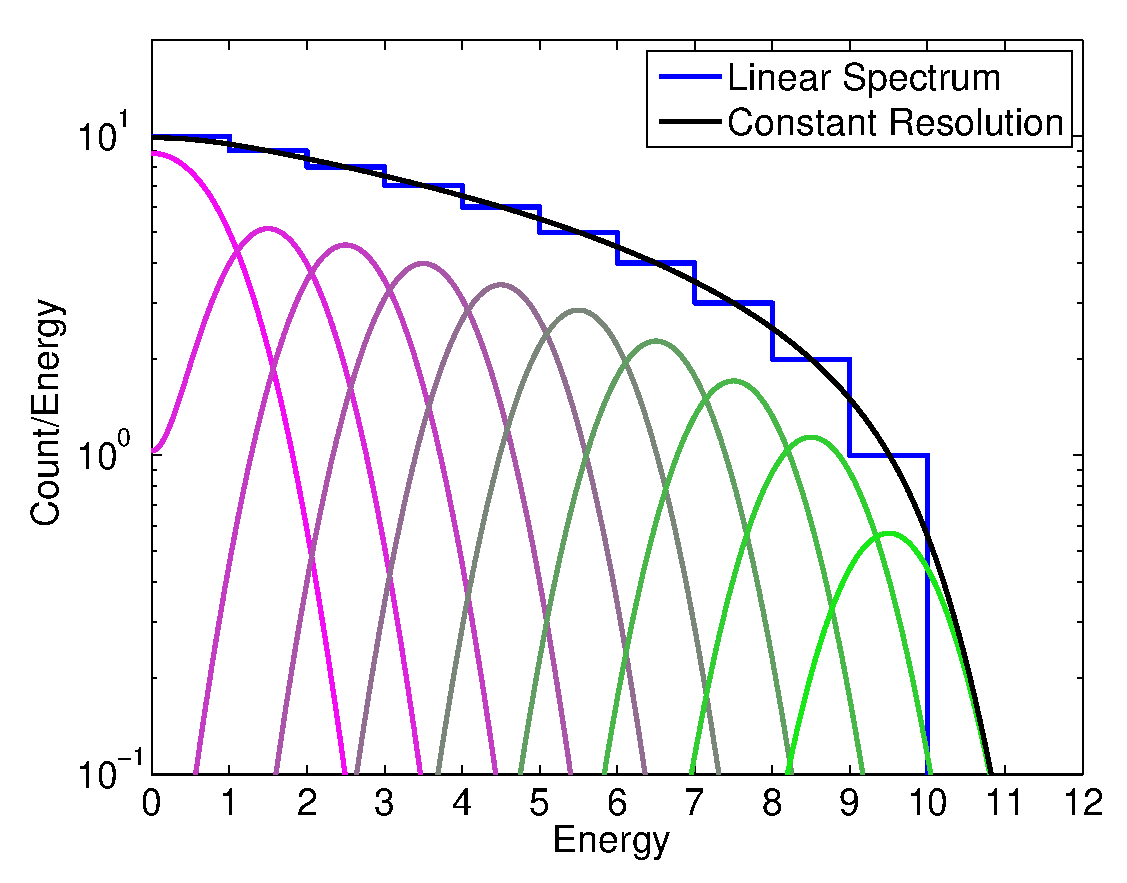
\includegraphics[width=70mm]{Figures/Toy_Model_lin_const}
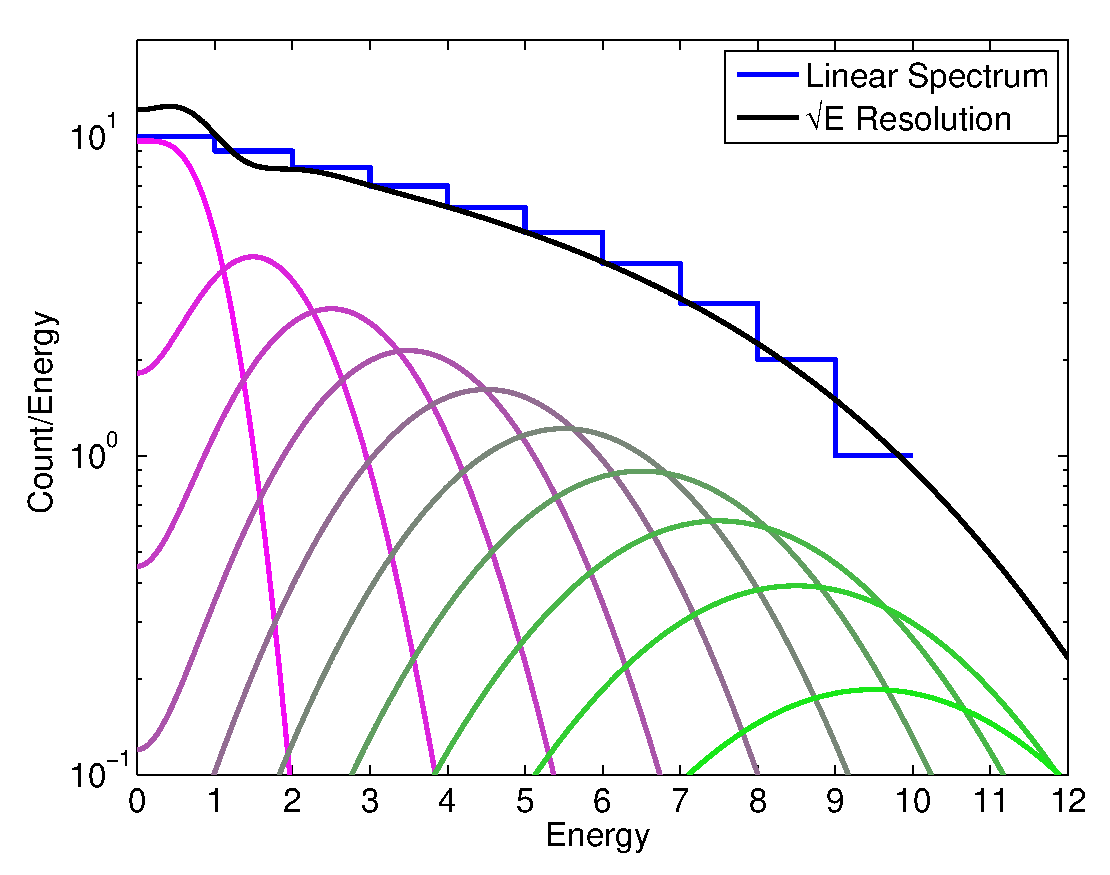
\includegraphics[width=70mm]{Figures/Toy_Model_lin_dep}
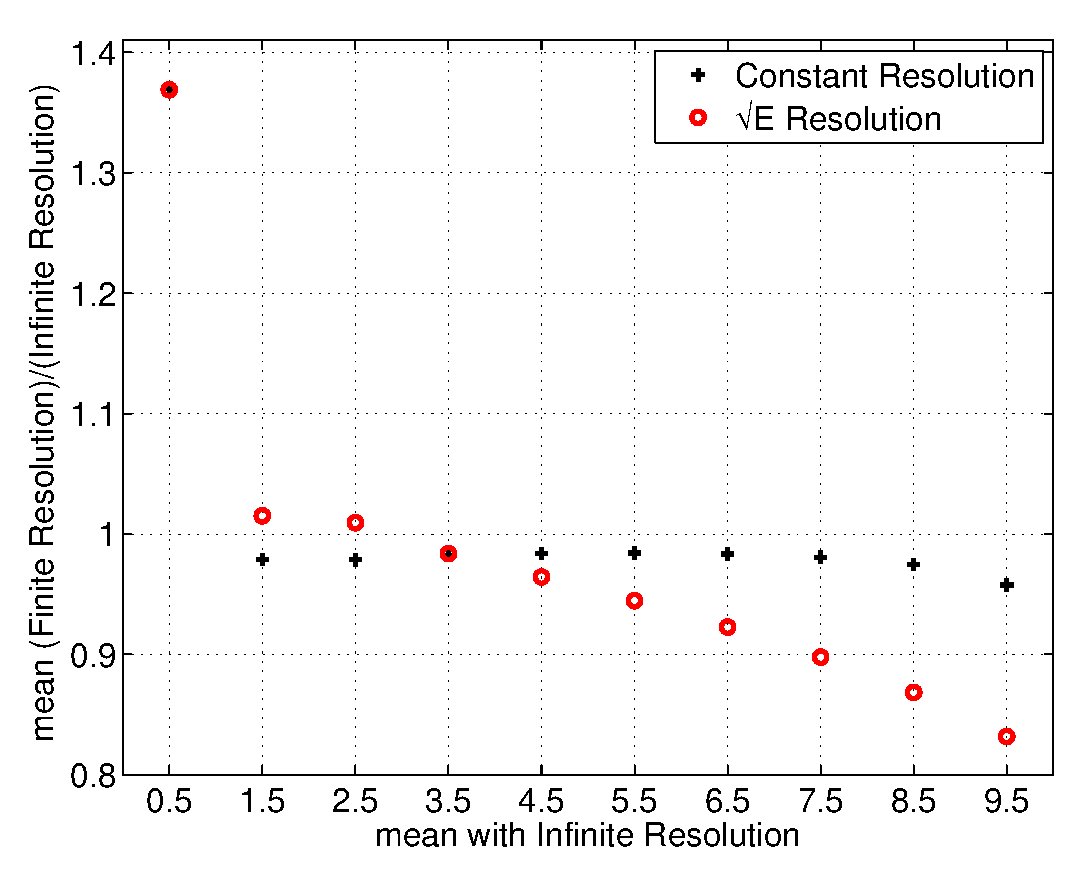
\includegraphics[width=70mm]{Figures/Toy_Model_mean_shift}
\caption{Top Left: A linearly decaying spectrum, in blue. The black curve represents the sum of the Gaussians assuming a constant resolution. Top Right: A linearly decaying spectrum, in blue. The black curve represents the sum of the Gaussians with a $\rm \sqrt{E}$ dependent resolution. Bottom: The observed mean, with finite resolution, compared to the real mean with infinite resolution. The black points are for the case with linear resolution and the red points represent the case with $\rm \sqrt{E}$ dependent resolution.}
\label{fig:Toy_Linear}
\end{figure}



\subsection{Correcting the Tritium S1 Mean}

The correction for the mean of the measured light yield, S1 [Phe], for tritium beta decay can be solved for using equation \ref{eq:5}. Starting with a simulated S1 tritium spectrum with infinite resolution and applying equations \ref{eq:1}-\ref{eq:5} one can attain the mapping of measured mean to true mean. The resolution of S1 was determined empirically from X-ray and $\rm^{83}Kr$ gammas, see table \ref{table:Var}. The use of Gaussian error down to low S1 is an acceptable approximation since underlying distribution actually consists of the number of photons, $\rm n_\gamma = \frac{S1}{g1}$. With g1=0.138 there are still 15 photons near the S1 threshold of 2 [Phe], thus the Gaussian model is still a close approximation of the underlying Poisson distribution. We will use the Gaussian approximation as it makes the application of equations \ref{eq:1}-\ref{eq:5} much simpler.
Using equation \ref{eq:Fano} and \ref{eq:Gain} we can solve for the the spread in S1 as a function of S1 and its corresponding energy \ref{eq:S1_res}. The spread in S1 is the result of the variation in the recombination fluctuations at a given energy, thus it requires an energy dependent coefficient F(E).
\begin{equation}
 \rm \sigma_{S1}=F(E)\sqrt{S1\times g1}
\label{eq:S1_res}
\end{equation}

Figure \ref{fig:S1_mapping} shows the application of smearing applied to the S1 tritium spectrum. The shift in the spectral shape, back and red, is hardly noticeable however, the shift in observed mean from the real mean is non negligible.


 \begin{figure}[h!]\centering
\includegraphics[width=80mm]{Figures/S1_comp_smear_LUX_SIM_Tritium}
%\includegraphics[width=80mm]{Figures/S1_smear_comp}
\includegraphics[width=80mm]{Figures/S1_corr_.eps}
\caption{Top: In Black, a simulated tritium photon spectrum. In red, the mean of the spectrum after applying finite energy resolution of equation \ref{eq:5}. Bottom Left: Mapping of the observed mean, with finite resolution, to the mean with infinite resolution for a tritium photon spectrum. Bottom Right: The ratio of the real mean to the observed mean vs. the observed mean for a tritium photon spectrum. Note the S1 threshold at about 2 Phe in S1. }
\label{fig:S1_mapping}
\end{figure}


\subsection{Correcting the Tritium S2 Mean}

The correction for the mean of the measured light yield, S1 [Phe], for tritium beta decay can be solved for using equation \ref{eq:5}. Starting with a simulated S2 tritium spectrum with infinite resolution and applying equations \ref{eq:1}-\ref{eq:5} one can attain the mapping of measured mean to true mean.  The energy resolution of S1 was determined empirically to be $\rm \sigma_{S1} = 10.6 \sqrt{S2} $, from $\rm^{83}Kr$ the combined gammas at 41.6 [keV]. The use of Gaussian error down to low S2 is an acceptable approximation since the S2 spectrum ends at 300 [Phe], $\rm n_e = \frac{S2}{g2}$. With g2=6.54 there are still 20 electrons near end of the tritium spectrum, thus the Gaussian model is still a close approximation of the underlying Poisson distribution. We will use the Gaussian approximation as it makes the application of equations \ref{eq:1}-\ref{eq:5} much simpler.
Using equation \ref{eq:Fano} and \ref{eq:Gain} we can solve for the the spread in S2 as a function of S2 and its corresponding energy \ref{eq:S2_res}. The spread in S2 is the result of the variation in the recombination fluctuations at a given energy, thus it requires an energy dependent coefficient F(E).

\begin{equation}
 \rm \sigma_{S2}=F(E)\sqrt{S2\times g2}
\label{eq:S2_res}
\end{equation}


Figure \ref{fig:S2_mapping} shows the application of smearing applied to the S2 tritium spectrum. 

 \begin{figure}[h!]\centering
\includegraphics[width=80mm]{Figures/S2_comp_smear_LUX_SIM_Tritium}
\includegraphics[width=80mm]{Figures/S2_corr.eps}
\caption{Top: In Black, a simulated tritium electron spectrum. In red, the mean of the spectrum after applying finite energy resolution of equation \ref{eq:5}. Bottom Left: Mapping of the observed mean, with finite resolution, to the mean with infinite resolution for a tritium electron spectrum. Bottom Right: The ratio of the real mean to the observed mean vs. the observed mean for a tritium electron spectrum. Note the S2 threshold is around 500 Phe, due to the S1 threshold at 2 Phe.}
\label{fig:S2_mapping}
\end{figure}


\subsection{Correcting the Tritium Energy Spectrum}

The mapping of the observed energy to real energy was determined using a full simulation of tritium beta decay. The accuracy of the smearing model described in equations \ref{eq:1}-\ref{eq:5} can be tested by comparingit against the energy observed after a full NEST simulation. The energy depends on both S1 and S2 thus, mapping observed energy to true energy my be non trivial. Again, we start with a simulated tritium energy spectrum with infinite resolution and apply the empirically determined resolution in equation \ref{eq:E_res}, measured with $\rm^{127}Xe$ X-rays and $\rm ^{83m}Kr$ calibrations. Figure \ref{fig:E_spec} shows the comparison of smearing model vs true energy along with the smearing after running full photon and electron propagation in LUXSIM vs the true energy. The smearing form the model described in equations \ref{eq:1}-\ref{eq:5} is almost identical to the output of LUXSIM. The energy spectrum flares out at low energy, is pulled in from 5-10 [keV] and again flares out slightly above 15 [keV]. It is important to note that the change in the spectral shape is hardly noticeable, as was the case with S1 and somewhat with S2. Figure \ref{fig:E_mapping} shows the results for mapping observed energy to real energy using both smearing methods. The two methods show good agreement down to the threshold of 1.5 [keV], the agreement with simulation is always within 1\%. Below 2 [keV] the model predicts the ratio of true energy to observed energy to rise as there are greater number of events at higher energy spilling over to lower energy, the simulation however does not show this behavior leading to a 5\% discrepancy in the 1 [keV] bin. We take the difference between the smearing model and LUXSIM as a systematic uncertainty. 

Using equation \ref{eq:Fano}, \ref{eq:Gain} and \ref{eq:E_res1} we solve for the the spread in E as a function energy \ref{eq:E_res}. F(E) is the measure of the variance in recombination fluctuations, with values interpolated from table \ref{table:Var}. W=73 [$\rm \frac{N_{quanta}}{keV}$].

\begin{gather}
\label{eq:E_res1} \rm E= \frac{1}{W}(n_\gamma + n_{e^-}) \\
 \rm \sigma E^2= \frac{1}{W^2}(\sigma n_\gamma ^2 + \sigma n_{e^-} ^2)\\ 
 \rm \sigma E^2= \frac{1}{W^2}(F(E)^2 n_\gamma + F(E)^2 n_{e^-})\\
 \rm \sigma E^2= \frac{F(E)^2}{W}\frac{(n_\gamma + n_{e^-})}{W}\\
 \rm \sigma E^2= \frac{F(E)^2}{W}E\\
  \rm \sigma E= \frac{F(E)}{\sqrt{W}}\sqrt{E}
\label{eq:E_res}
\end{gather}



 \begin{figure}[h!]\centering
\includegraphics[width=80mm]{Figures/E_comp_smear_LUX_SIM_Tritium.eps}
\includegraphics[width=80mm]{Figures/E_hist_LUX_SIM_Tritium.eps}
\caption{MC vs. Data, with detector threshold. And smeared MC vs all MC without a detector threshold. }
\label{fig:E_spec}
\end{figure}


 \begin{figure}[h!]\centering
\includegraphics[width=80mm]{Figures/E_density_LUX_SIM_Tritium.eps}
\includegraphics[width=80mm]{Figures/E_corr.eps}
\caption{Left, mapping from real Monte Carlo energy to observed energy after applying a finite resolution using LUXSIM. Right, comparing the correction determined from the Monte Carlo (Red) to the smearing model (black). The dashed lines represent the uncertainty in the measured value of F(E). The agreement is within errors from 1 to 18 keVee. The Energy threshold is near 1.0 keVee.}
\label{fig:E_mapping}
\end{figure}

\newpage

\section{The Standard Candle. Light Yield from $\rm^{83m}Kr$}

Quenching of scintillation yield vs. field has been  typically defined relative to 32.1 keV decay of $\rm^{83m}Kr$ at zero field \cite{Aprile_LY},\cite{Baudis}. $\rm^{83m}Kr$ first emits a 32.1 [keV] gamma followed by a 9.4 [keV] with a half life of 154 [ns] between the two (refs). The combined signal (41.6 [keV]) is found by the pulse finder in the majority of cases, using the standard WIMP search pulse gap setting of 500 ns. However, the combined signal is not useful as a standard calibration since the light yield from the second 9.4 keV decay depends strongly on decay time separation. The second 9.4 keV decay is effected by the presence of exitons from the initial 32.1 [keV] decay. See figure [ show LUX result]

Fortunately, the first 32.1 keV appears to have no time dependance as it decays in `relaxed' xenon without the presence of additional exitons \cite{Aprile_LY}. For purposes of light yield normalization at zero field the 32.1 keV gamma serves as a good low energy standard candle for xenon detectors.

There were two data sets in late 2013 that contain $\rm^{83m}Kr$ decays at zero field. Since the S2 (charge) signal is unavailable the top-bottom asymmetry, $\frac{top-bottom}{top+bottom} $, is used to define the Z coordinate for position dependent corrections. The XY correction is subdominant to the Z dependent correction for light yield. Figure [] shows the linear mapping from top-bottom asymmetry to detector depth (Z). With the Z correction applied the average pulse area (Phe) normalized to the detector center (241.6 mm below the gate grid) is found to be $\rm 267.4 \pm^{stat} 1.5 \pm^{sys} 5$. See Figure \ref{fig:ZeroField_Kr}.

 
 \begin{figure}[h!]\centering
\includegraphics[width=80mm]{Figures/S1_Z_no_field_lux10_20131009T1358_cp06914}
\includegraphics[width=80mm]{Figures/dT_no_field_2lux10_20131009T1358_cp06914}
\caption{Left: $\rm^{83m}Kr$ peaks at zero field. ** The 9.4 keV peak is fit only for events with a decay time separation greater than 1000 [ns]. Right: shows the timing separation between the 32.1 and 9.4 [keV] decays plotted above.}
\label{fig:ZeroField_Kr}
\end{figure}
 
\subsection{Field dependence of light yield from the 32.1 keV gamma of $\rm ^{83m}Kr$ }

Charge separation increases with drift field leading to less recombination for light production, causing scintillation yield to be quenched. See table \ref{table:kr32} for a list of the measured scintillation of the 32.1 keV gamma from $\rm ^{83m}Kr$, also includes the NEST predictions.

\begin{table}[h!]
\begin{center}
\begin{tabular}{|c|c|c|c|c|c|}
\hline
Field [V/cm]	&S1[Phe]	& Photons[$n_{\gamma}$]	& Yield [$n_{\gamma}$/keV	]	&NEST	   [$n_{\gamma}$/keV]\\ \hline
0 	&	267.4 $\pm$ 6.5 	&1980 $\pm$ 40.7 &	61.7 $\pm$	1.27 	&	64.2 $\pm$ 2.6  \\ \hline
51 &	246.7 $\pm$ 1.2 	&1827.4 $\pm$ 8.9 & 	56.9 $\pm$	0.28	 &	60.8 $\pm$ 2.5 \\ \hline
105 &	233.6 $\pm$ 1.4 	&1730.4 $\pm$ 	10.4 &	53.9 $\pm$ 0.32 	&	58.3 $\pm$ 2.3 \\ \hline
182 & 212.3 $\pm$ 1.3	&1572.6 $\pm$ 	9.6  &	49.0 $\pm$0.30 	&	54.9 $\pm$ 2.1 \\ \hline
\end{tabular}
\caption{Field dependance of the light yield form the 32.1 keV decay of $\rm^{83m}Kr$. The fields are calculated using a two dimensional model and not accounting potential charge accumulation on inner teflon panels.}
\label{table:kr32}
\end{center}
\end{table}



%\begin{table}[h!]
%\begin{center}
%\begin{tabular}{|c|c|c|c|c|c|c|}
%\hline
%Field 	&41.6 [keV] 	& 32.1 [keV] 	& 9.4* [keV] 	&9.4** [keV] & S2	&S2 ** \\ 
% \[[V/cm]	&	S1[Phe]	&S1[Phe]	&S1[Phe]&		S1[Phe]		&S2[Phe]		&S1[Phe]  \\ \hline
%0 	&		359.9 $\pm$ 5	 			&267.4 $\pm$ 6.5 		&78 $\pm$ 2	 	&	 92.5$\pm$	6 		&	--  			& --	\\ \hline
%51 &		332.6 $\pm$ 1.4 			&246.7 $\pm$ 1.2 		&76.4 $\pm$ 0.5 	& 	86 $\pm$ 1		 &	3651 $\pm$ 5	& 3708 $\pm$ 11 \\ \hline
%105 &		316.8 $\pm$ 1.4 			&233.6 $\pm$ 1.4 		&72.9$\pm$ 0.5		 &	83 $\pm$ 1 			&	4357 $\pm$ &4399 $\pm$ 16 \\ \hline
%182	 & 		291.3 $\pm$ 1.4 			&212.3 $\pm$ 1.3		&68.8 $\pm$ 0.5 	&	79 $\pm$ 1 		&	4986 $\pm$ 5 	 &5048$\pm$ 13 \\ \hline
%\end{tabular}
%\caption{Field dependance of the light yield form the 32.1, 9.4 and combined 41.6 [keV] decay of $\rm^{83m}Kr$. The fields are calculated using a two dimensional model and not accounting potential charge accumulation on inner teflon panels. ** *}
%\end{center}
%\label{table:krAll}
%\end{table}


\newpage
\section{Scintillation Yield and Ionization Yield from Tritium Beta Decay}

\subsection{Cuts used in this analysis}

\begin{itemize}
\item Standard LIX Pulse finder classifier used in the WIMP search.
\item $\rm S2_b > 100 [Phe] $
\item PDE (g1) = 0.138 $\rm \pm 0.005$, measured with Tritium
\item Extraction = 0.655 $\rm \pm 0.02$ measured with Tritium.
\item single e- = 9.95 $\rm \pm 0.1$ [Phe/e-]
\item Using NEST 4c bands.
\end{itemize}



\subsection{Results at 180 [V/cm], Corrected for Spectral Shape}

See Figures \ref{fig:L_Q_Yield} and \ref{fig:L_Q_Yield_180}.

The scintillation and ionization yield is defined as [Photons/keV] and [Electrons/keV] respectively. For conversion of pulse area to photons and electrons along with the combined energy calculation see section []. The measurement was made using a triturated methane calibration source which provides betas ranging from $\rm>1$ to about 18 [keV]. Over 150,000 beta decay events, in the fiducial volume, were used to measure scintillation and ionization yield at 180 [V/cm]. Figure \ref{fig:L_Q_Yield} shows the results from the tritium calibration before correcting for the shape of the tritium spectrum.

\begin{figure}[h!]\centering
\includegraphics[width=120mm]{Figures/LY_c_180_Tritium_Dec_2013_Charge_Yield_180_corr.png}
\includegraphics[width=120mm]{Figures/CH3T_fid_E_S2_c_Tritium_Dec_2013_Charge_Yield_180_corr.png}
\caption{Top: Scintillation yield vs. combined enery using tritium beta decay. Bottom: Ionization yield vs. combined energy using tritium beta decay. At a drift field of 180 [V/cm], in the fiducial volume, and containing over 150,000 beta decays. The S1, S2 and  energy has been corrected for spectral shape and detector resolution. The endpoint of the tritium beta spectrum is 18.6 [keV]. }
\label{fig:L_Q_Yield}
\end{figure}


 \begin{figure}[h!]\centering
\includegraphics[width=82mm]{Figures/LY_180_band_Tritium_Dec_2013_Charge_Yield_180_corr.png}
\includegraphics[width=82mm]{Figures/QY_180_Tritium_Dec_2013_Charge_Yield_180_corr.png}
\includegraphics[width=83mm]{Figures/LY_180_band_log_Tritium_Dec_2013_Charge_Yield_180_corr.png}
\includegraphics[width=76mm]{Figures/QY_180_log_Tritium_Dec_2013_Charge_Yield_180_corr.png}
\caption{180 [V/cm], corrected for spectral shape. Top Left: Mean scintillation yield vs. combined energy using tritium beta decay (black line). $\rm^{83}Kr$ lines are plotted for reference but only the 32.1 [keV] line (red star) is kosher since the 9.4 [keV] line is dependent on timing separation, the 9.4 [keV] line is plotted (blue star) for separations greater than 1000 [ns]. Top Right: Mean ionization yield vs. combined energy (black line). Bottom Left: Scintillation yield vs. combined energy on a log scale. Bottom Right: Ionization yield vs. combined energy on a log scale. The shaded blue regions represent the NEST mean with $\pm 5\%$ that has been vetted by data [Erik Dahl Thesis]. The shaded magenta regions represent the NEST extrapolations from data. The measurement is made at a field of 180 [V/cm] and contains over 150,000 beta decays. The endpoint of the tritium beta spectrum is 18.6 [keV]}
\label{fig:L_Q_Yield_180}
\end{figure}


\subsection{Results at 100 [V/cm], Corrected for Spectral Shape}

... See Figure \ref{fig:L_Q_Yield_100}.


 \begin{figure}[h!]\centering
\includegraphics[width=82mm]{Figures/LY_100_Tritium_Dec_2013_Yield_100_corr}
\includegraphics[width=81mm]{Figures/QY_100_Tritium_Dec_2013_Yield_100_corr}
\includegraphics[width=83mm]{Figures/LY_180_band_log_Tritium_Dec_2013_Yield_100_corr}
\includegraphics[width=76mm]{Figures/QY_180_log_Tritium_Dec_2013_Yield_100_corr}
\caption{105 [V/cm], corrected for spectral shape. Top Left: Mean scintillation yield vs. combined energy using tritium beta decay (black line). $\rm^{83}Kr$ lines are plotted for reference but only the 32.1 [keV] line (red star) is kosher since the 9.4 [keV] line is dependent on timing separation, the 9.4 [keV] line is plotted (blue star) for separations greater than 1000 [ns]. Top Right: Mean ionization yield vs. combined energy (black line). Bottom Left: Scintillation yield vs. combined energy on a log scale. Bottom Right: Ionization yield vs. combined energy on a log scale. The shaded blue regions represent the NEST mean with $\pm 5\%$ that has been vetted by data [Erik Dahl Thesis]. The shaded magenta regions represent the NEST extrapolations from data. The measurement is made at a field of 100 [V/cm] and contains about 5,000 beta decays. The endpoint of the tritium beta spectrum is 18.6 [keV]}
\label{fig:L_Q_Yield_100}
\end{figure}



\subsection{Compared With recent Compton Scattering Measurement}

... See Figure \ref{fig:L_Q_Yield_Baudis}.

 \begin{figure}[h!]\centering
\includegraphics[width=100mm]{Figures/Re_all_log_T_paper_corr_threshold.eps}
\includegraphics[width=80mm]{Figures/LY_all_T_paper.eps}
\includegraphics[width=80mm]{Figures/Charge_Y_all_Tritium_Dec_2013_Charge_Yield_180_corr.eps}
\caption{Top: Scintillation yield relative to the yield of the 32.1 gamma of [keV] $\rm^{83}Kr $  vs. Energy. Shaded blue curve is tritium at 100 [V/cm], shaded black curve is tritium at 180 [V/cm], red points represent a recent Compton scattering measurement at 450 [V/cm]. Also shown are the corresponding quenching of the 32.1 [keV]  gamma of $\rm^{83}Kr$ (star inside circle). Bottom: scintillation yield [Photons/keV] vs. Energy. Shaded blue curve is tritium at 100 [V/cm], shaded black curve is tritium at 180 [V/cm], red circles represent a recent Compton scattering measurement at 450 [V/cm].}
\label{fig:L_Q_Yield_Baudis}
\end{figure}

\newpage
\section{Fixing the Low Energy Tritium `Pile Up' }

By modifying the scintillation yield down and ionization yield up at low energy the strange `pile up' at low energies can be resolved. 

\begin{figure}[h!]\centering
\includegraphics[width=80mm]{Figures/CH3T_E_dis_Tritium_Dec_2013_Yield_180_corr.png}
\includegraphics[width=80mm]{Figures/CH3T_S1_dis_zoom_Tritium_Dec_2013_Yield_180_corr}
%\includegraphics[width=77mm]{Figures/CH3T_ER_NEST_Tritium_Dec_2013_Charge_Yield_180.png}
\caption{With S1 and S2 spectral shape correction. Left: log10(S2/S1) (black) and NEST (shaded blue) vs. Energy. The data and the NEST prediction agree between 1[keV] to 8 [keV], where the NEST model is optimized. Right: log10(S2/S1) (black) plotted vs S1. The shaded blue region represents the NEST mean with $\pm 5\%$. that has been vetted by data [Erik Dahl Thesis]. The shaded magenta regions represent the NEST extrapolations from data. The deviation at low S1 is potentially due to greater ionization yield than predicted by NEST at low energy.}
\label{fig:L_Q_Yield_180_NEST}
\end{figure}

\begin{figure}[h!]\centering
\includegraphics[width=84mm]{Figures/CH3T_E_dis_Tritium_Dec_2013_Charge_Yield_180}
\includegraphics[width=75mm]{Figures/CH3T_S1_dis_zoom_Tritium_Dec_2013_Charge_Yield_180}
%\includegraphics[width=77mm]{Figures/CH3T_ER_NEST_Tritium_Dec_2013_Charge_Yield_180.png}
\caption{No spectral shape correction. Left: log10(S2/S1) (black) and NEST (shaded blue) vs. Energy. The data and the NEST prediction agree between 1[keV] to 8 [keV], where the NEST model is optimized. Right: log10(S2/S1) (black) plotted vs S1. The shaded blue region represents the NEST mean with $\pm 5\%$  The deviation at low S1 is potentially due to greater ionization yield than predicted by NEST at low energy.}
\label{fig:L_Q_Yield_NEST_2}
\end{figure}


 \begin{figure}[h!]\centering
\includegraphics[width=100mm]{Figures/CH3T_E_spec_218_Tritium_Dec_2013_Charge_Yield_180}
\caption{Tritium Data along with LUX SIM,  the `pile up' at low energy seen in all previous tritium energy specta can be solved by modifying charge yield and light yield at low energies.}
\label{fig:L_Q_Yield_NEST_3}
\end{figure}


\newpage
\section{Discrimination vs E and S1}

\subsection{Discrimination vs. S1}

 \begin{figure}[h!]\centering
\includegraphics[width=80mm]{Figures/CH3T_fid_50_Tritium_Dec_2013_S2_100Phe_cut}
\includegraphics[width=80mm]{Figures/CH3T_Leakage_fid_50_Tritium_Dec_2013_S2_100Phe_cut}
\caption{Discrimination vs. S1. On average from 0 to 50 Phe the discrimination is 99.50\%, defined by the number of events of events below the mean of the nuclear recoil band. The red band represents the NEST nuclear recoil band (version 4c).}
\label{fig:Dis_S1}
\end{figure}

\subsection{Discrimination vs. Combined Energy}

 \begin{figure}[h!]\centering
\includegraphics[width=80mm]{Figures/CH3T_fid_E_Tritium_Dec_2013_S2_100Phe_cut}
\includegraphics[width=80mm]{Figures/CH3T_Leakage_E_fid_50_Tritium_Dec_2013_S2_100Phe_cut}
\caption{Discrimination vs. combined energy. On average from 0 to 6.5 keV (0-50 Phe  S1) the discrimination is 99.46\%, defined by the number of events of events below the mean of the nuclear recoil band. The red band represents the NEST nuclear recoil band (version 4c).}
\label{fig:Dis_S1}
\end{figure}




\bibliographystyle{thesisbibstyle}
\bibliography{TritiumBib}



\end{document}
